\documentclass[MSc]{abdnthesis}                                           

\usepackage[super,sort&compress]{natbib}
\usepackage{placeins}
\usepackage{url}
\setlength{\bibsep}{0pt}
\bibliographystyle{unsrt}

\usepackage[T1]{fontenc}

\title{Measuring Martian winds by tracking clouds in Emirates Mars Mission UV imaging}
\author{Victoria Lercher}
\school{Student ID: 52319275}    
\date{2024}

%% If you want to include only a couple of chapters then use the
%% \includeonly{} command with a list of the file/chapter names that
%% you wish to include.  NB, this must be in the preamble.

\includeonly{introduction, data, methods, results, conclusion, references, appendix}

\def\sfthing#1#2{\def#1{\mbox{{\small\normalfont\sffamily #2}}}}

\sfthing{\PP}{P}
\sfthing{\FF}{F}

\begin{document}

\maketitle
\makedeclaration

\begin{abstract}
Understanding wind patterns on Mars is crucial for future human exploration and for enhancing our knowledge of planetary climate dynamics. Despite its significance, Martian winds are still considered a major unknown. This thesis seeks to contribute to filling this gap by utilizing six image sequences from the Emirates Mars Mission's EXI 320 nm ultraviolet observations. A cloud tracking method, Correlation Image Velocimetry (CIV), was employed to derive wind field maps with a time separation of 10 – 30 minutes. Various image processing techniques were tested to potentially optimize CIV performance, and their impacts on the resulting wind fields were analyzed. 
Using the results obtained from the image sequences pre-processed with contrast limited adaptive histogram equalization (CLAHE), wind fields were compared to those derived in a previous thesis by Shaimaa Ahmed AlBlooki, published in 2023. Her study used three of the same image sequences, but relied on an older version of the image data that was not pointing corrected. Key findings include that while different pre-processing methods in this thesis had a minimal impact on CIV performance overall, CLAHE-processed image sequences resulted in the detection of more velocity vectors compared to differently processed sequences. Additionally, although there are some discrepancies between the wind fields presented here and those in Al Blooki's study, the general wind direction trends remain consistent.
\linebreak
\linebreak
\textbf{Keywords:} Mars, Atmosphere, Cloud Tracking, Correlation Imaging Velocimetry 
(CIV), Image processing, Wind Fields. 
\end{abstract}

\tableofcontents
\listoftables
\listoffigures

\chapter{Introduction\label{chap:introduction}}

With many Earth-like features such as obliquity seasons (“summer” and “winter”), polar ice caps, a similar rotation period, and evidence suggesting that liquid water once existed on its surface\cite{clancyetalChapter022017}, Mars is an intriguing subject of study, which can help us understand how physical processes interact to shape a planet’s climate and drive its changes\cite{Leovy1978}. A key factor driving climatic processes on Mars is wind and atmospheric circulation. It has not only shaped Mars' surface over time but plays a crucial role in the transport of water vapor, dust, trace gases, and heat. Although understanding wind patterns is highly relevant for future human exploration, they are still considered a major unknown\cite{Guzewich2021}.

\section{Historical Background}

The earliest efforts to determine wind flows on Mars, published in 1950 by Seymour Hess, were based on pixelated photographs taken during the planet's northern hemisphere winter, yielding 18 wind vectors as shown in Figure 1.1\cite{Seymour1950}. 
\FloatBarrier
\begin{figure}[h!] 
    \centering
    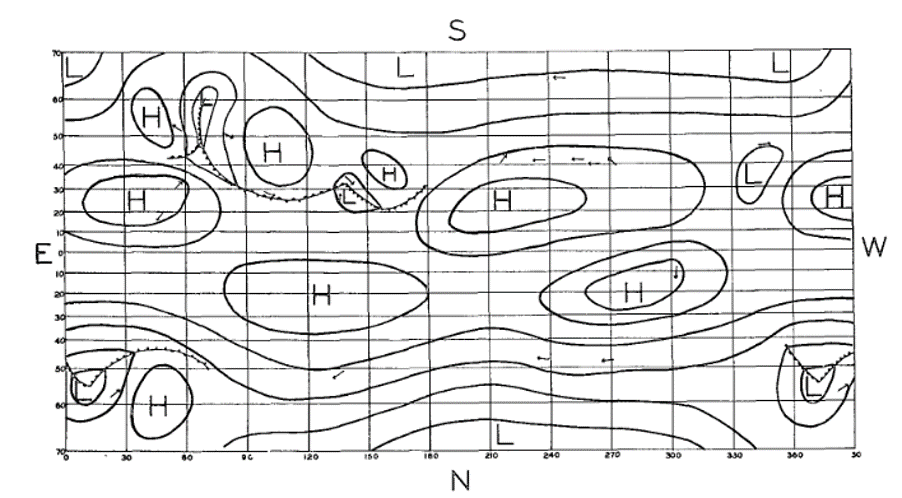
\includegraphics[width=1\textwidth]{fig_01.png}
    \caption{A schematic streamline map for Mars in northern hemisphere winter by Seymour Hess, where arrows represent observed cloud drift directions\cite{Seymour1950}. }
\end{figure}
\FloatBarrier
However, as technology progressed, instrumental capabilities gradually improved. The launch of the Hubble Space Telescope in 1990 provided high-resolution ultraviolet and visible light images taken above the distorting effects of the Earth’s atmosphere\cite{Uri2020}, enabling a detailed, pixel-based longitude-wise analysis of the Martian aphelion cloud belt\cite{Wolff1999}. The successful landing of Pathfinder in 1997 marked the introduction of on-surface measurements, as it recorded atmospheric data during its descent and conducted meteorological measurements at the landing site\cite{NasaMarsPathfinder}. While on-surface measurements from Pathfinder and subsequent missions like the Mars Exploration Rover and Phoenix Mars Lander offer excellent local coverage, orbital observations, which began with the Mars Global Surveyor in 1988 and continued with missions such as NASA's Mars Odyssey and Mars Reconnaissance Orbiter\cite{clancyetalChapter022017}, provide global coverage that facilitates the analysis of wind patterns on a larger scale.

\section{Cloud Tracking}

While the idea of tracking clouds using planetary-type imagery has been around since Robert Hooke observed a moving spot in one of the belts of Jupiter in the 16th century\cite{Hooke1665}, non-manual tracking of atmospheric motion was properly established as a practice in the 1960s, shortly after the first meteorological satellites were launched\cite{Menzel2001}. Since then, various tracking methods have evolved and been applied across diverse fields of research requiring motion tracking. Among these, optical flow and cross-correlation algorithms have emerged as techniques delivering efficient results not only in studies of e.g. fluid mechanics but also in large-scale cloud tracking in planetary atmospheres. 




\chapter{Data\label{chap:data}}

One of the recent missions that enables remote wind measurements and serves as the data source for this thesis, is the Emirates Mars Mission (EMM), which was launched in 2020 and entered Mars orbit in 2021. The mission is equipped with three scientific instruments: the Emirates Mars InfraRed Spectrometer (EMIRS), the Emirates Mars Ultraviolet Spectrometer (EMUS), and the Emirates eXploration Imager (EXI)\cite{Amiri2022}.

\section{Relevance}

Among the various instruments and techniques available for atmospheric measurements from orbit, high-resolution images in ultraviolet wavelengths, such as those captured by the Emirates Mars Mission's EXI\cite{Jones2021}, are particularly valuable for tracking cloud movement, which is indicative of wind patterns. 
On Mars, the very low temperatures and pressures typically cause clouds to form as water ice. However, Martian clouds can also contain CO2 and display a wide range of properties and formations\cite{clancyetalChapter052017}. While visual observation of CO2 clouds is challenging, as they are mostly formed during the polar night, water ice clouds are more easily observed and are categorized into three broad regimes: the aphelion cloud belt (see Figure 2.1), polar hoods, and high-altitude haze (see Figure 2.2). The first two categories represent clouds in the lower atmosphere, below 40 km in altitude, while the third category is found at slightly higher altitudes, above 30–40 km\cite{clancyetalChapter052017}.
\FloatBarrier
\begin{figure}[h!] 
    \centering
    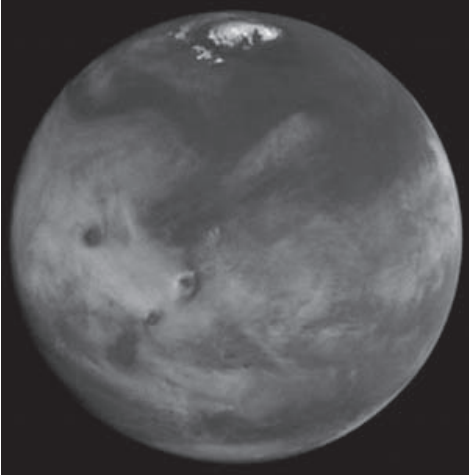
\includegraphics[width=0.5\textwidth]{fig_02.png}
    \caption{Hubble Space Telescope imagery capturing the Aphelion Cloud Belt on Mars\cite{clancyetalChapter052017}.}
\end{figure}
\FloatBarrier
\begin{figure}[h!] 
    \centering
    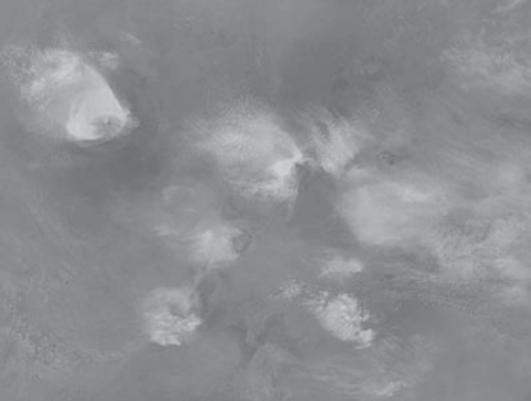
\includegraphics[width=0.5\textwidth]{fig_03.png}
    \caption{Typical afternoon cloud formations over Tharsis Montes during the northern summer (Ls = 122.3°)\cite{clancyetalChapter052017}.}
\end{figure}
\FloatBarrier
Since objective A of the Emirates Mars Mission focuses on characterizing the Martian lower atmosphere, the Emirates eXploration Imager (EXI) provides images that effectively display the altitudes where clouds are found\cite{Amiri2022}. An overview of Mars atmospheric layers mapped to EMM objectives can be seen in Figure 2.3. 
\FloatBarrier
\begin{figure}[h!] 
    \centering
    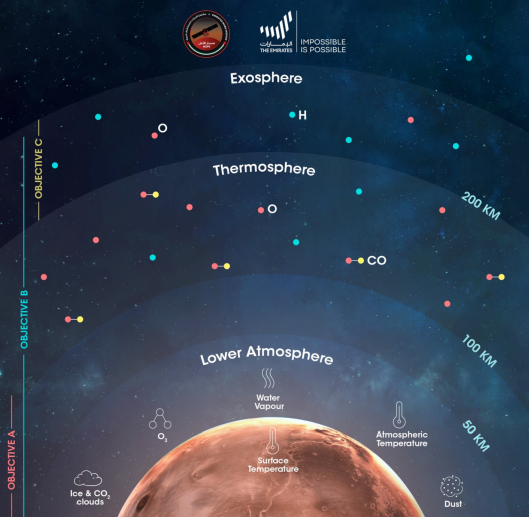
\includegraphics[width=0.8\textwidth]{fig_04.png}
    \caption{Illustration of Mars atmospheric layers mapped to EMM objectives and measurements\cite{Almatroushi2021}.}
\end{figure}
\FloatBarrier
EXI captures images across six bandpasses, centered at 220, 260, 320, 437, 546, and 635 nm, using two telescopes—one for ultraviolet (UV) and the other for visible (VIS) wavelengths, supporting different aspects of the mission's overall strategy. The full-disk images have a resolution of 2-4 km per pixel\cite{Jones2021}.

EXI’s ultraviolet imagery at 320nm is particularly well-suited for cloud tracking due to its focus on water ice optical depth. Water ice clouds have distinct absorption features in this UV spectrum, making them visible in the resulting images. Surface materials, however, do not reflect UV light at this wavelength. Consequently, any visible features, except for surface ice, are attributed to the lower atmosphere. This allows for a high degree of confidence in distinguishing atmospheric features in the UV images.

\section{Format}

The image sequences are provided in the form of FITS (Flexible Image Transport System) files, a format developed in the 1970s for archiving and exchanging astronomical data\cite{NasaFITS}. FITS files are designed to store data sets that include multidimensional arrays and two-dimensional tables. The data is organized in Header and Data Units (HDUs), which allow access to both the header containing general information and the data itself. The initial HDU is known as the Primary HDU. 
The chosen FITS files contain all data within the primary HDU. The data shape varies based on the number of images in each sequence, ranging from (6, 2880, 5760) to (22, 2880, 5760), where the first dimension indicates the number of images, and the second and third dimensions represent the height and width of the images. An illustration of the FITS file structure containing 6 images is shown in Figure 2.4. While the images are split between two bandpasses, only the images from the 320 nm bandpass were extracted for this thesis. 
\FloatBarrier
\begin{figure}[h!] 
    \centering
    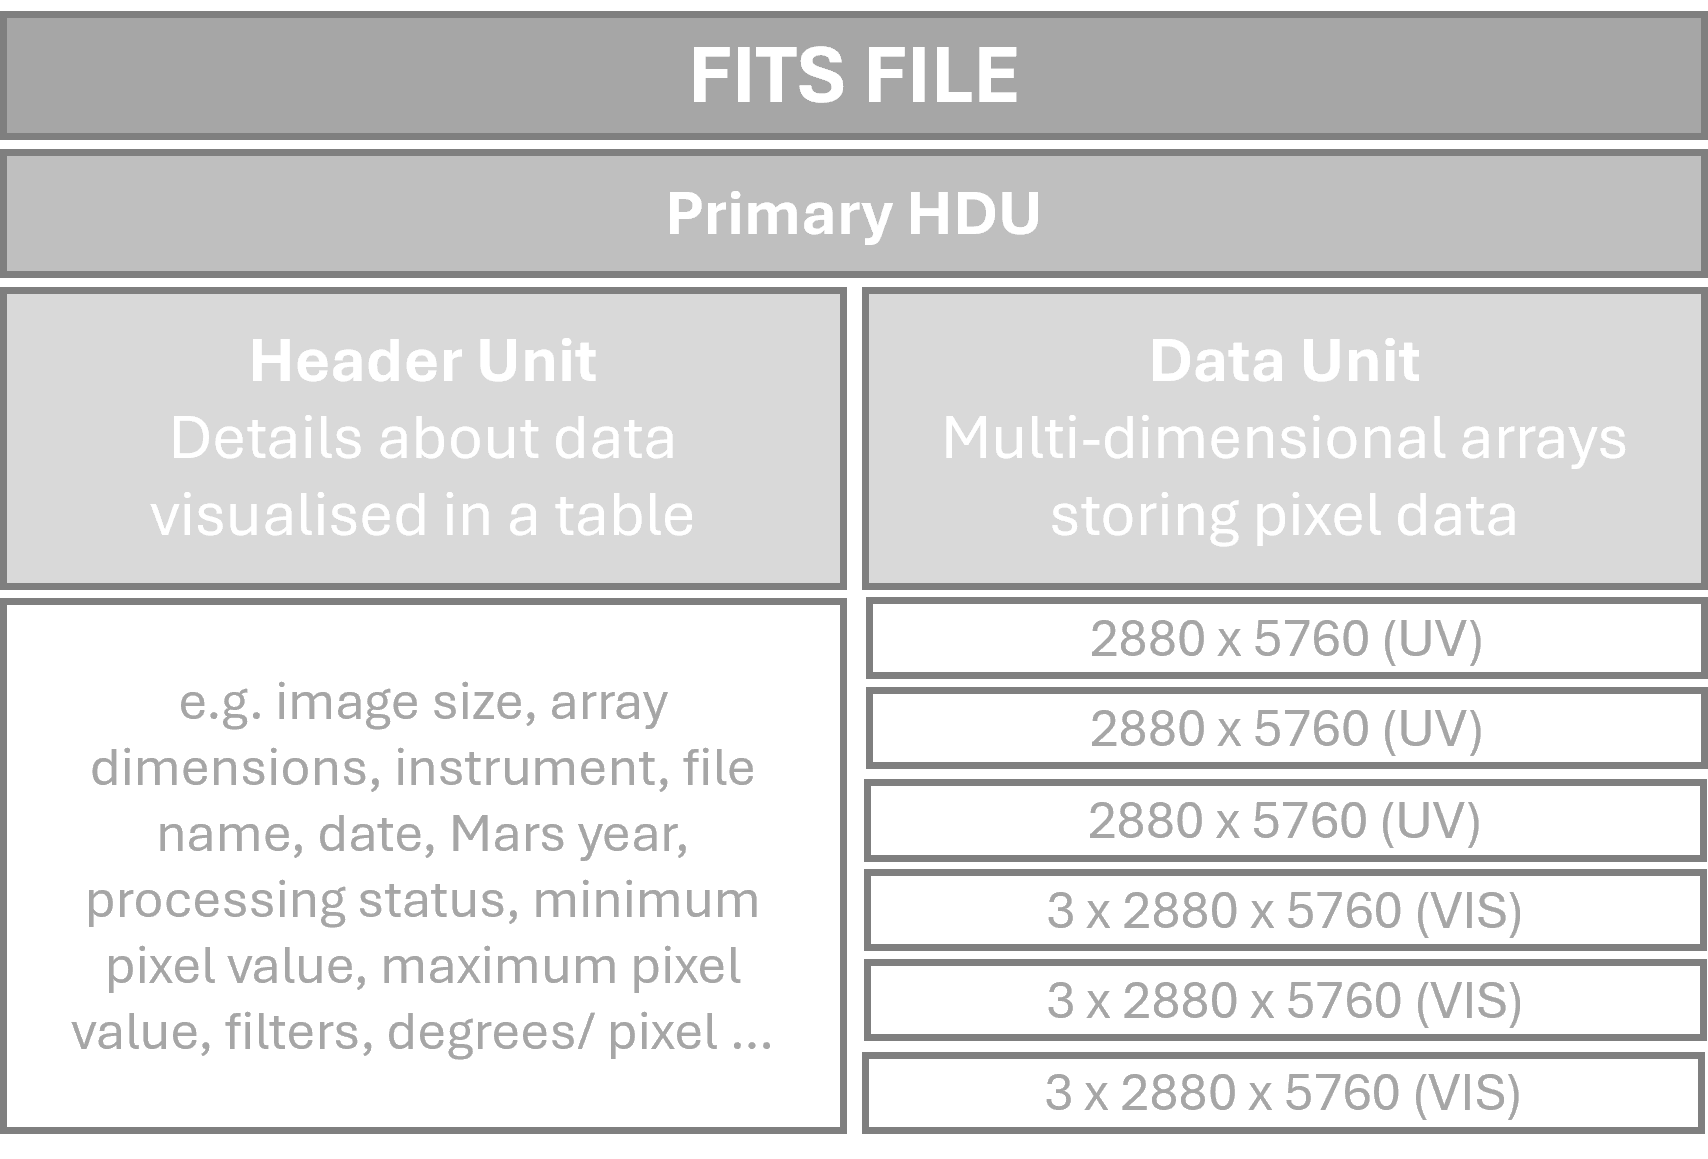
\includegraphics[width=0.8\textwidth]{fig_05.png}
    \caption{Visualization of a FITS file structure example including three visible (VIS) and three ultraviolet (UV) images.}
\end{figure}
\FloatBarrier
\section{Selection}

Among the available observation modes ranging from XOS1 to XOS14, the chosen image sequence is from XOS7 (EXI Observation Set 7). Additionally, the EXI data pipeline includes several product stages: L1 data (raw images), L2A (calibrated), L2B (map-projected), and L3 (retrievals)\cite{Jeppesen2021}. 

In a 2023 thesis by Shaimaa Ahmed AlBlooki, using UV imagery from the EXI instrument, it was identified that a jitter error (random motion) negatively impacted the accuracy of cloud tracking\cite{AlBlooki2023} (see Figure 2.5). This thesis utilizes recently released file versions, containing pointing corrected data, to mitigate jitter and improve precision of the cloud tracking.
\FloatBarrier
\begin{figure}[h!] 
    \centering
    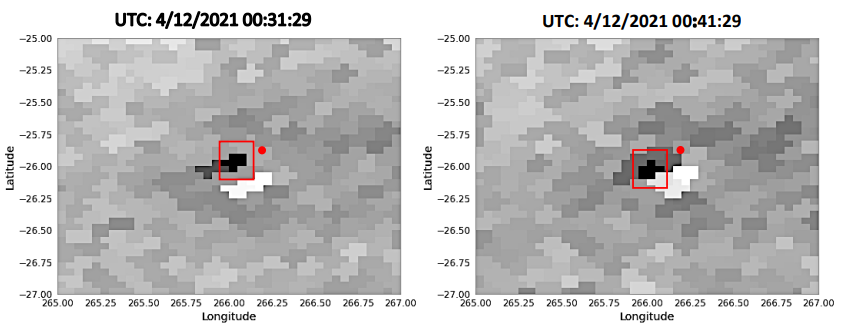
\includegraphics[width=1\textwidth]{fig_06.png}
    \caption{Example of jitter effect in older file version: EXI 635 nm XOS7 image, UTC: 4/12/2021 00:31:29-00:41:29\cite{AlBlooki2023}. The dot indicates the center of the frame. The images display a noticeable shift in crater positions.}
\end{figure}
\FloatBarrier
The selected image data set (Table 2.1) was captured during the northern summer solstice, within the solar longitude range of 131° to 146°. This period captures the aphelion cloud belt, characterized by its non-uniform cloud distribution (approx.14-50 km altitude) that begins forming around LS = 0°, reaches maximum optical depth around LS = 80°, and starts dissipating around LS = 140°. Typically, this cloud belt becomes longitudinally continuous by approximately LS = 60° and maintains this continuity until about LS = 140°, aligning with the solar latitudes of the chosen images\cite{clancyetalChapter052017}. 
\FloatBarrier
\begin{table}[h!]
    \centering
    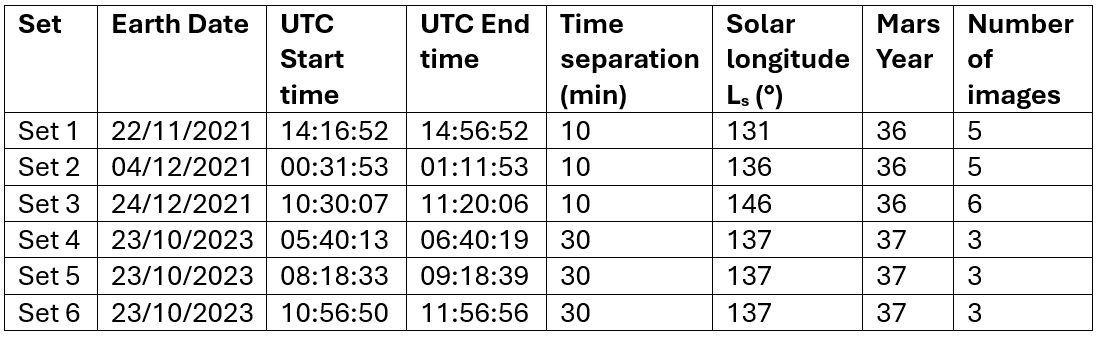
\includegraphics[width=1\textwidth]{table_01.png}
    \caption{List of set of images used in this thesis.}
\end{table}
\FloatBarrier
Shortly after the EXI mission began delivering data, images were captured at 5-minute intervals. In later sequences, the time separation increased to 30 minutes. While Sets 1, 2, and 3, captured in 2021 soon after data delivery commenced, were available with 5-minute intervals, the sequences used in this thesis were extracted at 10-minute intervals. This adjustment resulted in fewer images but was made to ensure higher accuracy in the cloud tracking process. Furthermore, the purpose of using the first three sequences is to enable comparison with results from an earlier thesis that used the same images, albeit without pointing correction\cite{AlBlooki2023}. The last three sets evaluate image sequences from 2023, providing a comparison two years later at a different time interval.
\FloatBarrier
\begin{figure}[h!] 
    \centering
    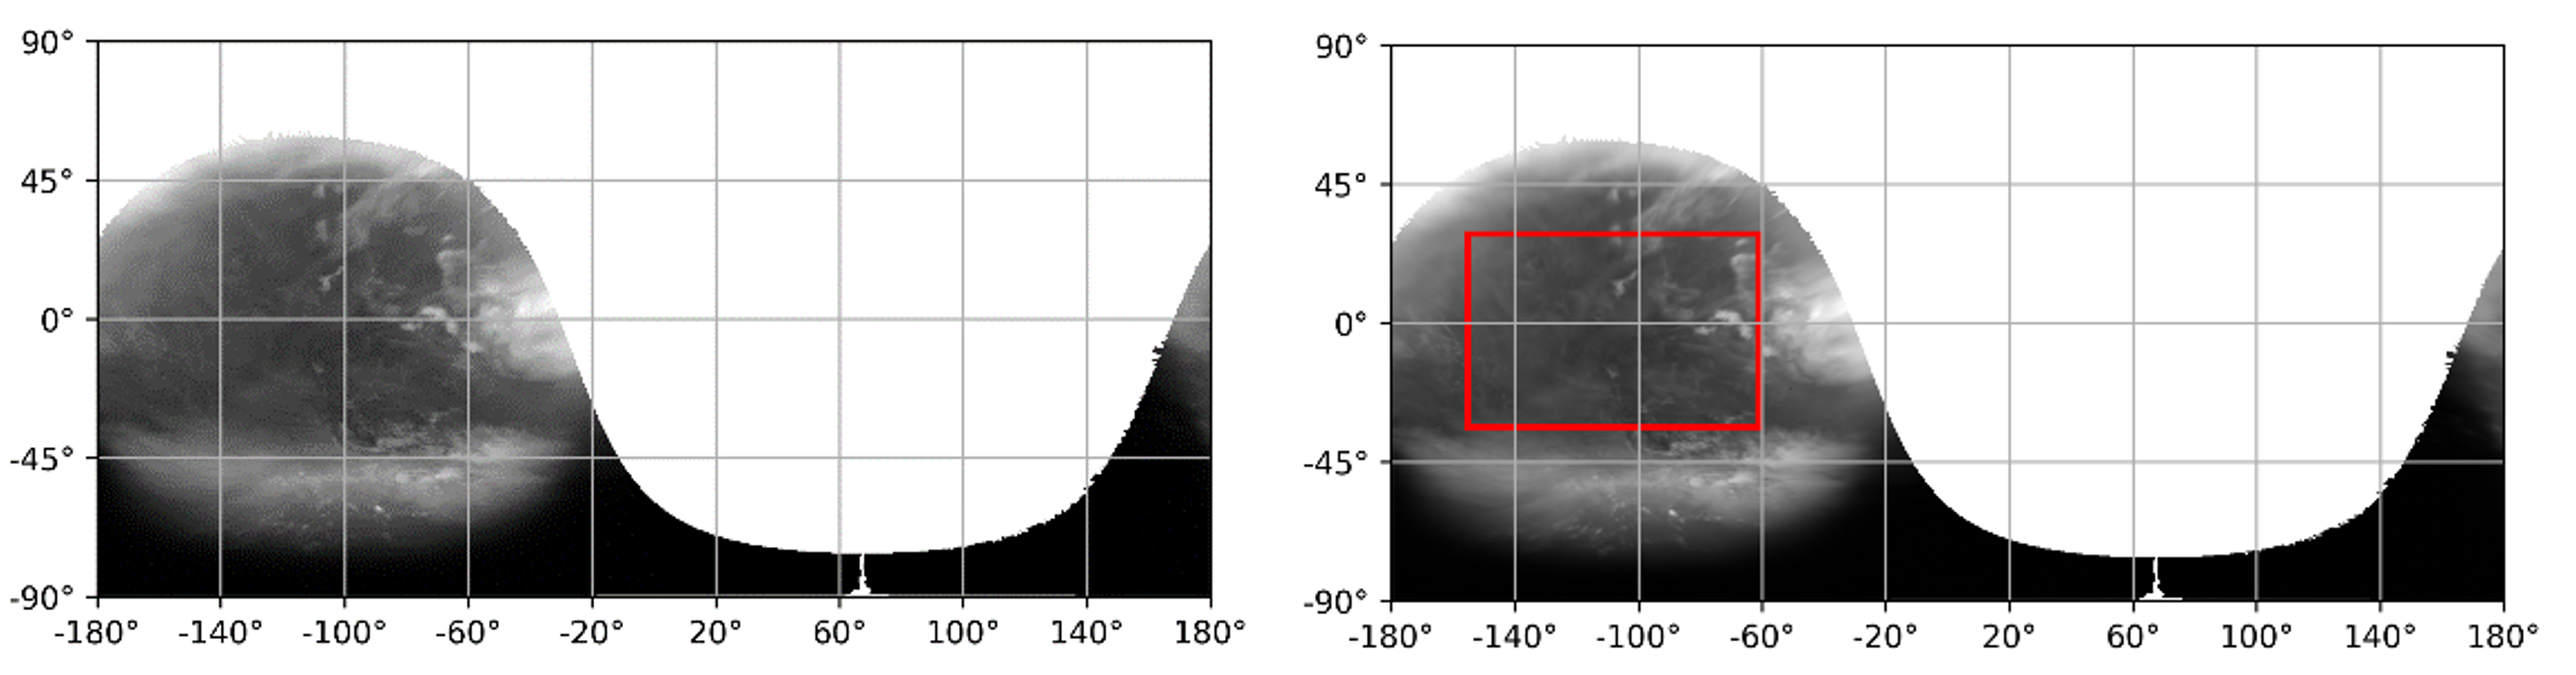
\includegraphics[width=1\textwidth]{fig_07.png}
    \caption{Example visualisation of the cropped area in images - UTC: 24/12/2021 10:30:07}
\end{figure}
\FloatBarrier
The images were cropped (see Figure 2.6) consistently across each sequence to exclude highly distorted areas at the edges of the hemisphere and regions that are not illuminated by the Sun. 
The resulting cropped regions cover longitudes from -167.5° to -23.75° and latitudes from -33.75° to 35°. An overview of these cropped regions is presented in Figure 2.7, and Table 2.2 details the latitude and longitude boundaries.
\FloatBarrier
\begin{figure}[h!] 
    \centering
    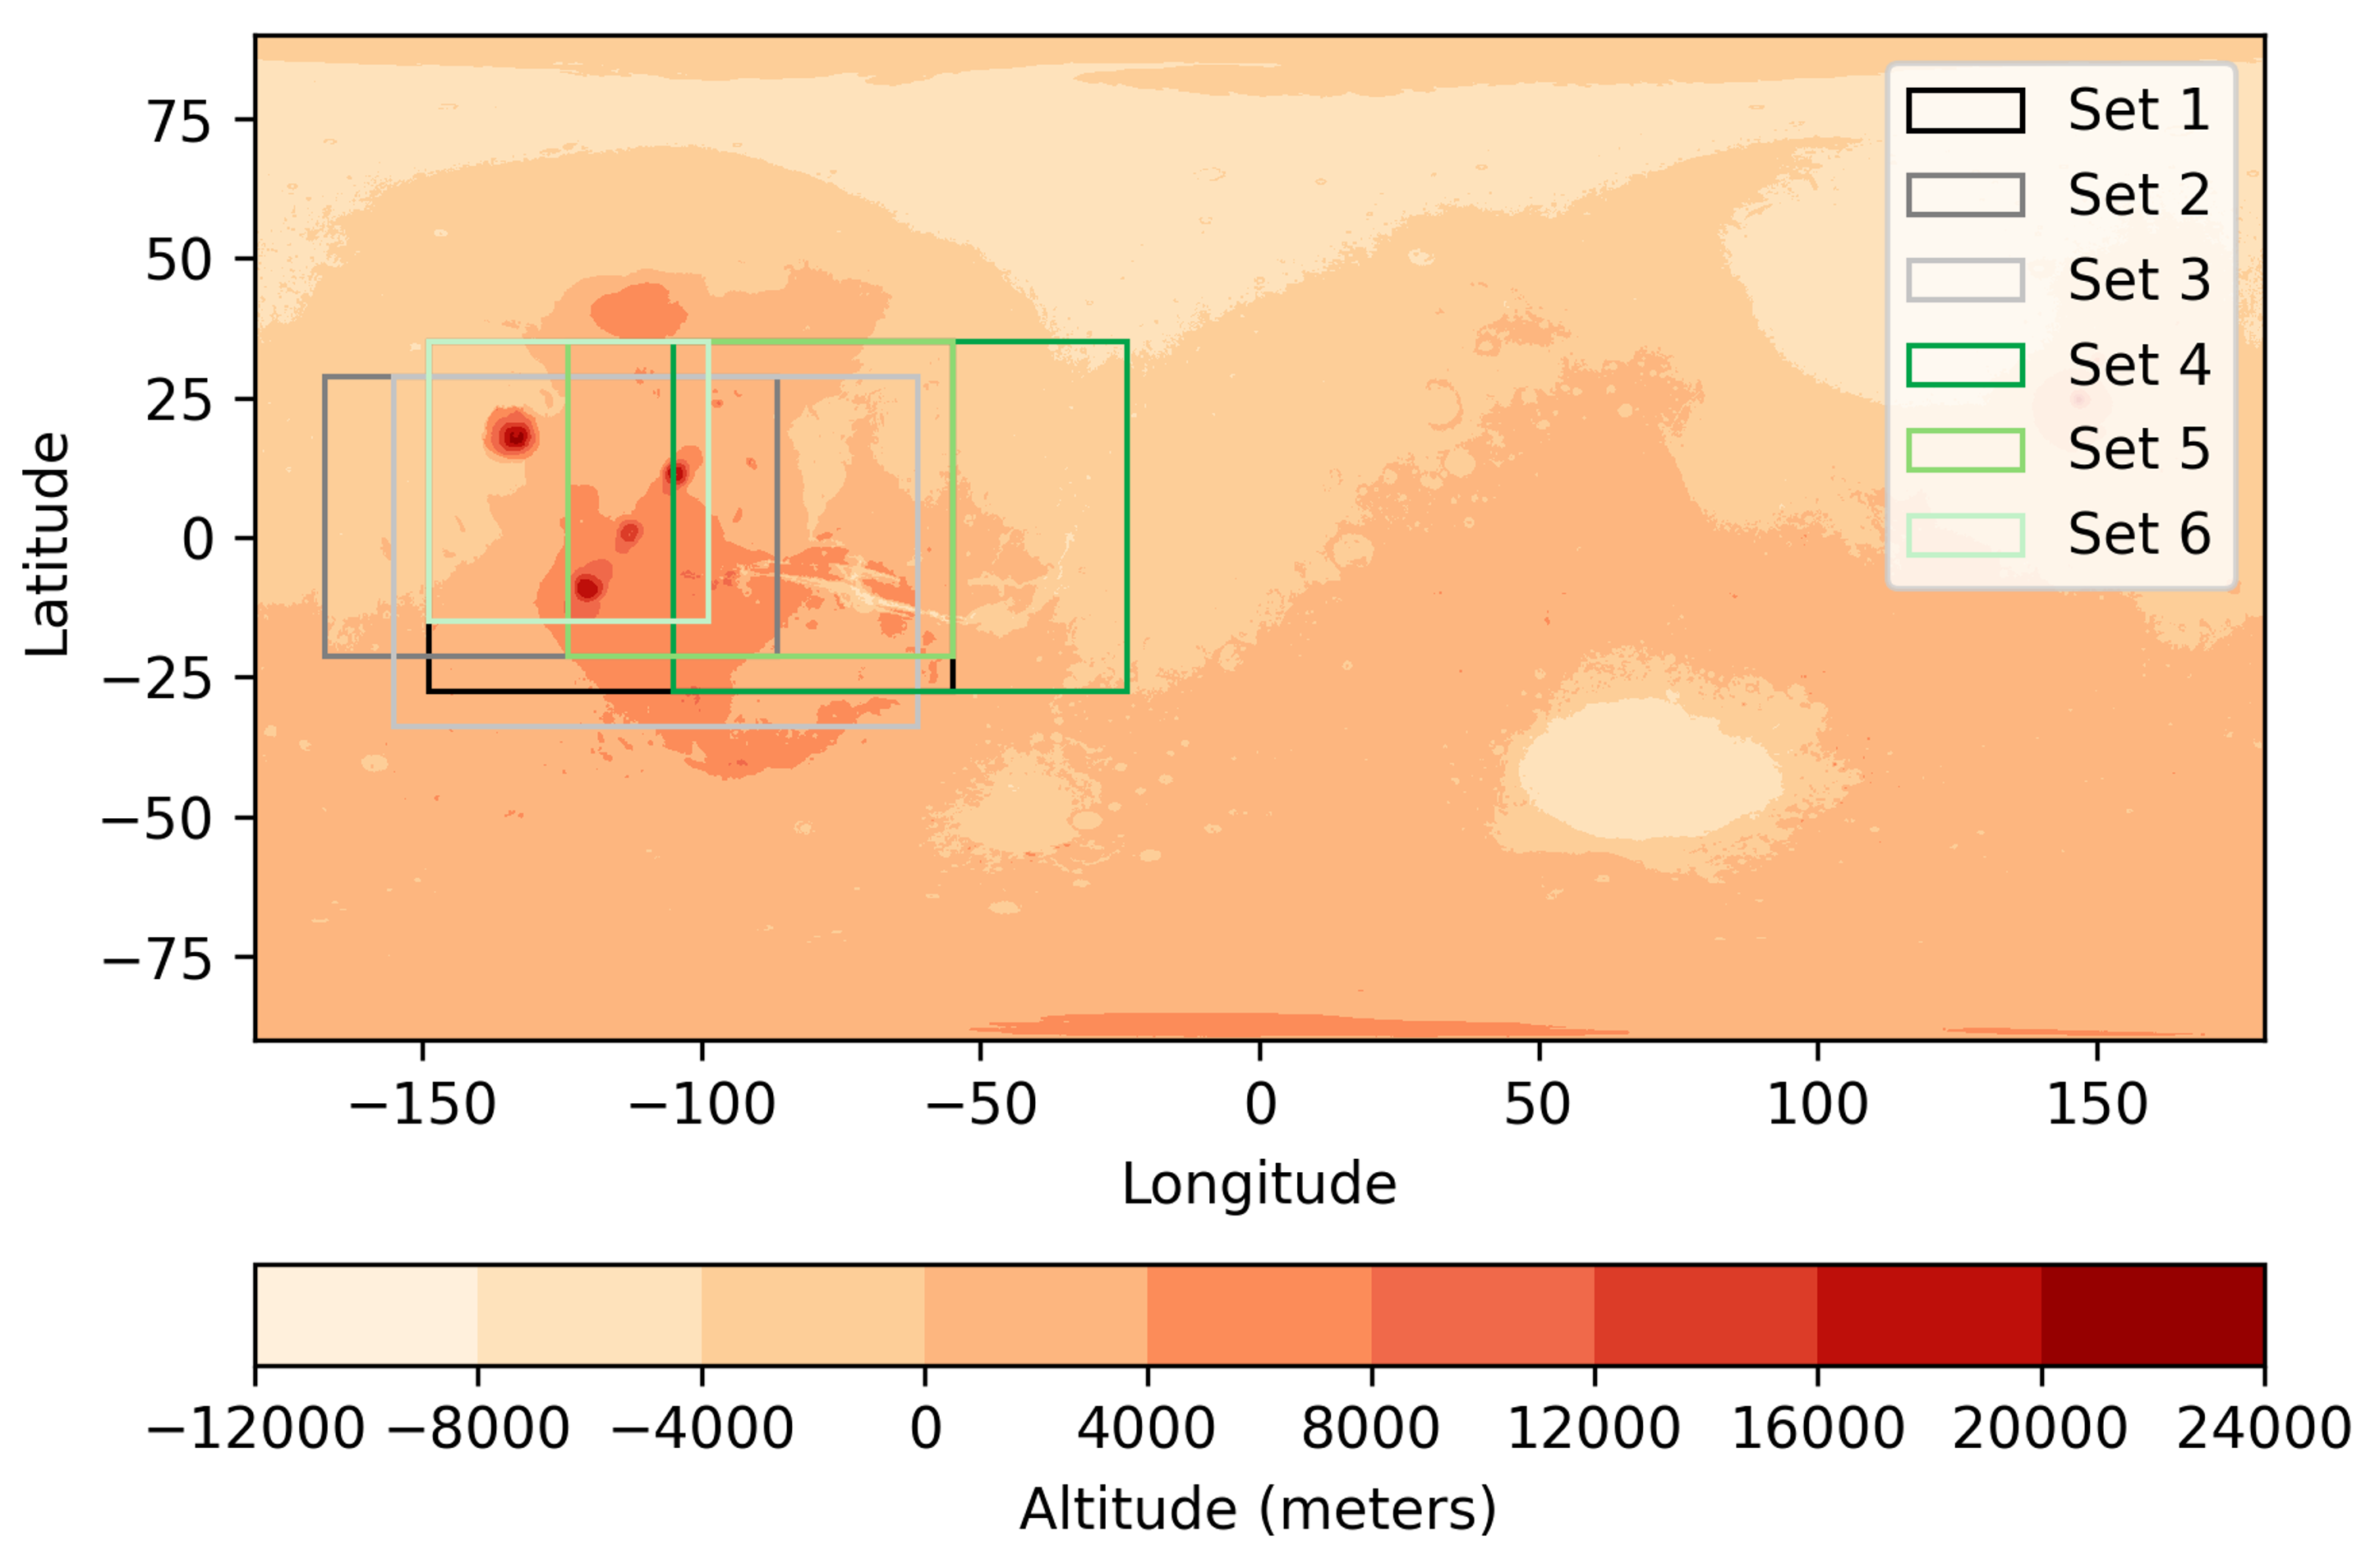
\includegraphics[width=1\textwidth]{fig_08.png}
    \caption{Illustration of the six areas of study using Mars Orbiter Laser Altimeter (MOLA) topography data\cite{MOLA}, where the red shades represent the topography of Mars and the frames indicate the cropped area for each image sequence.}
\end{figure}
\FloatBarrier
\begin{table}[h!]
    \centering
    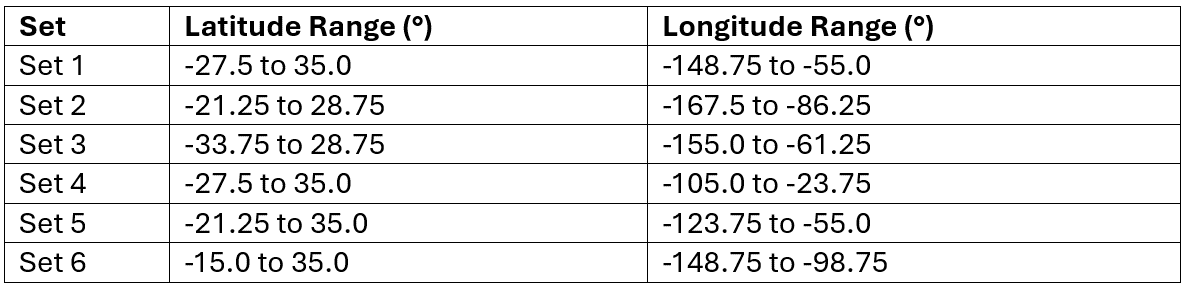
\includegraphics[width=1\textwidth]{table_02.png}
    \caption{ List of image sets cropped latitude and longitude ranges.}
\end{table}
\FloatBarrier
\section{Exploration}

The original projected UV images have a resolution of 2880 pixels in height and 5760 pixels in width, resulting in a total of 16.588.800 pixels. Of these, approximately 55 percent are NaN values, which represent areas not corresponding to Martian terrain. The remaining non-NaN pixels display a broad range of intensities, averaging between -24 and 3.930. The average intensity is approximately 819, with a median of 724 and a standard deviation of 796. The kurtosis and skewness of the pixel intensities are on average 0.08 and 0.79.
\FloatBarrier
\begin{figure}[h!] 
    \centering
    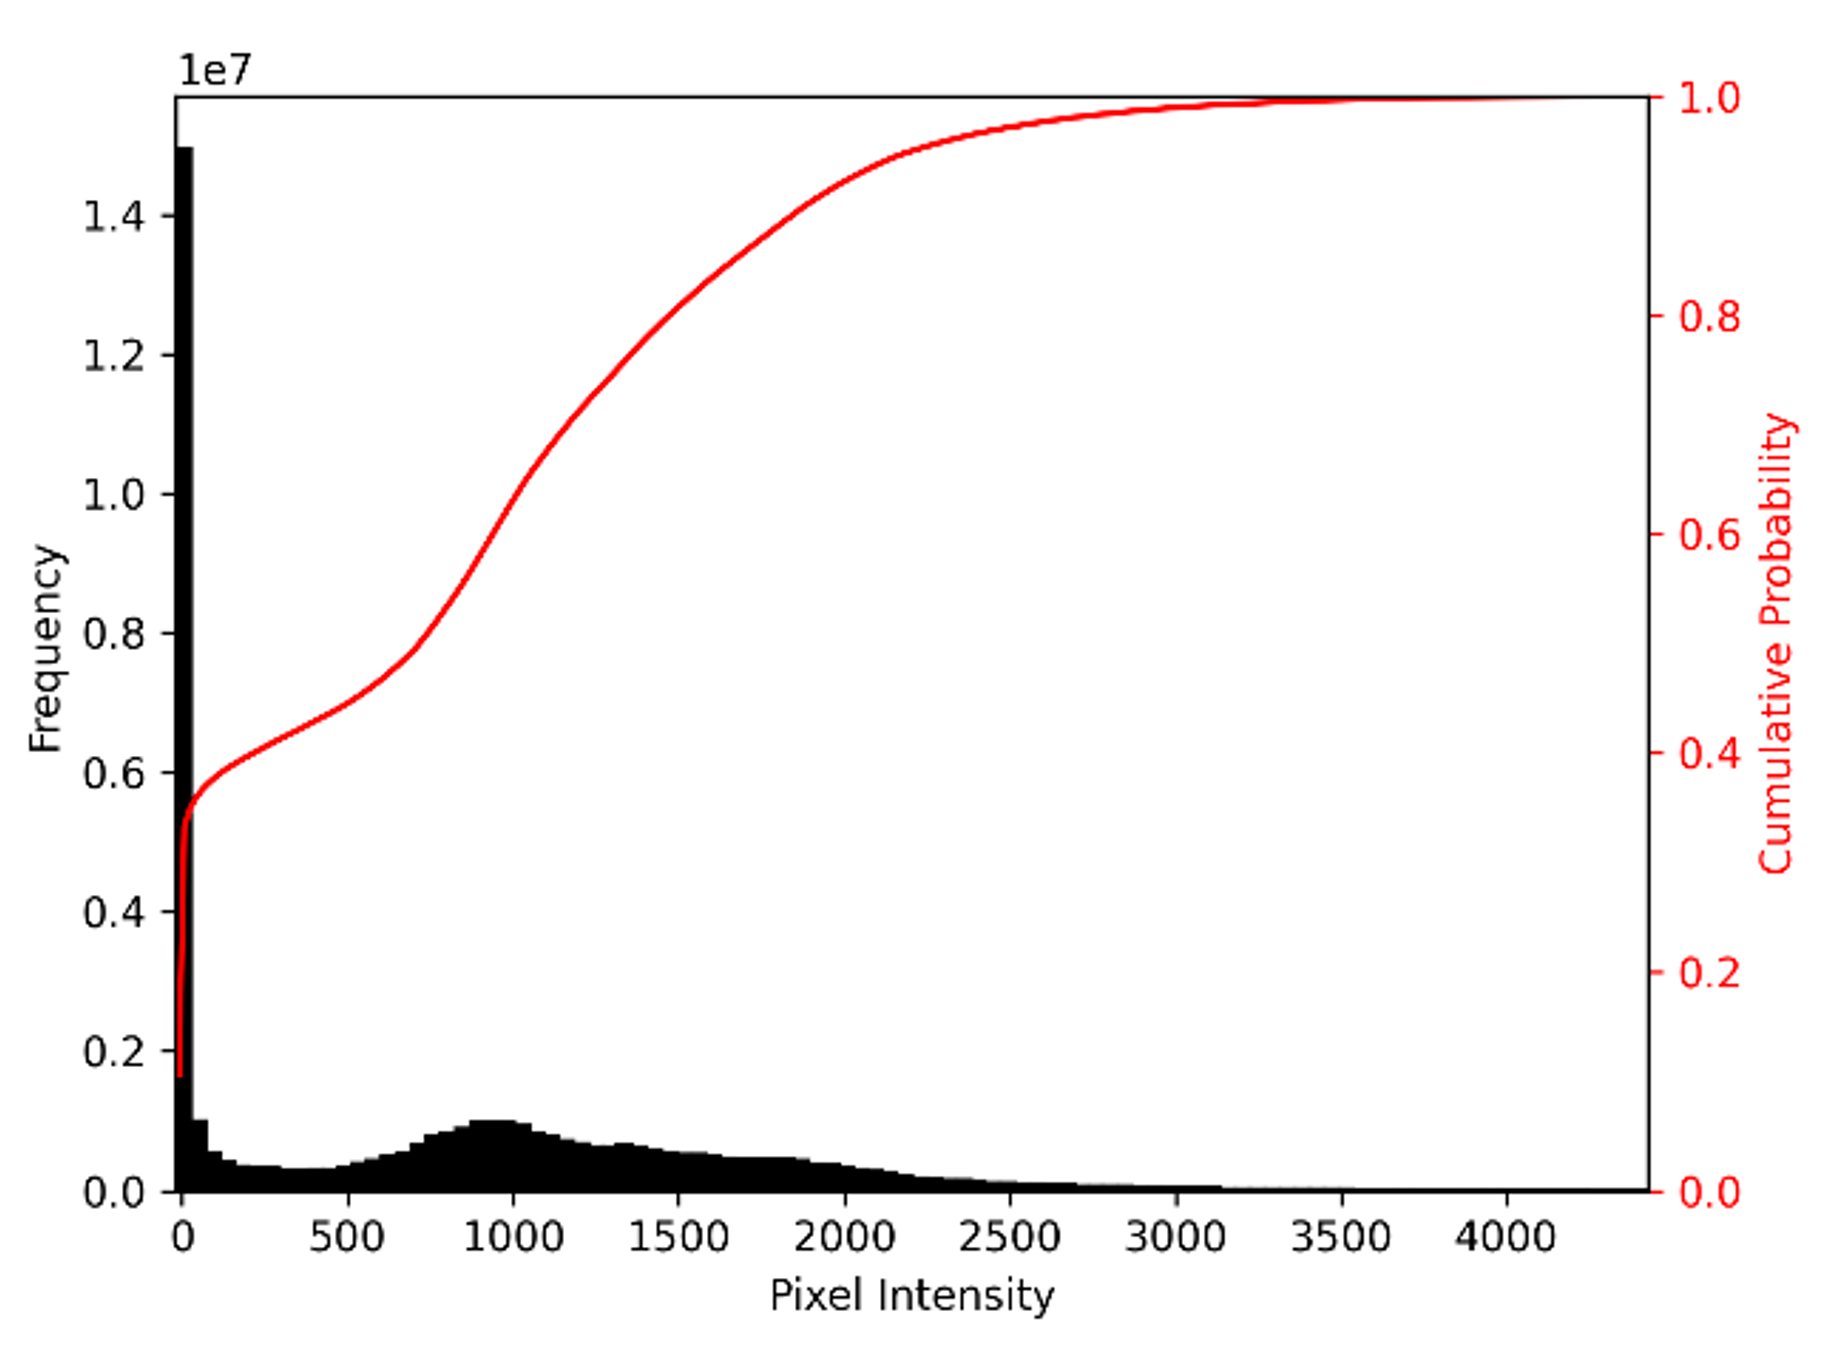
\includegraphics[width=0.8\textwidth]{fig_09.png}
    \caption{Visualization of the histogram and cumulative distribution of all selected image data across image sequences.}
\end{figure}
\FloatBarrier
Analysing the histogram and cumulative distribution function, shown in Figure 2.8, reveals that a significant proportion of pixel intensities are concentrated in the low range. Additionally, there is a noticeable peak in the lower-to-mid range of intensities, while higher intensity values are relatively sparse.

When reading the images back in Python, the “io.imread“ function from the “scikit-image” package normalized the pixel values to a range between 0 and 1, ensuring better readability in the subsequent analysis. The underlying equation for normalization is as follows:

\begin{equation}
\text{x}_{\text{normalized}} = \frac{x - x_{\text{min}}}{x_{\text{max}} - x_{\text{min}}}
\end{equation}

Where \( x_{\text{min}} \) represents the minimum intensity and \( x_{\text{max}} \) represents the maximum intensity of the image pixel data.
\FloatBarrier
\begin{figure}[h!] 
    \centering
    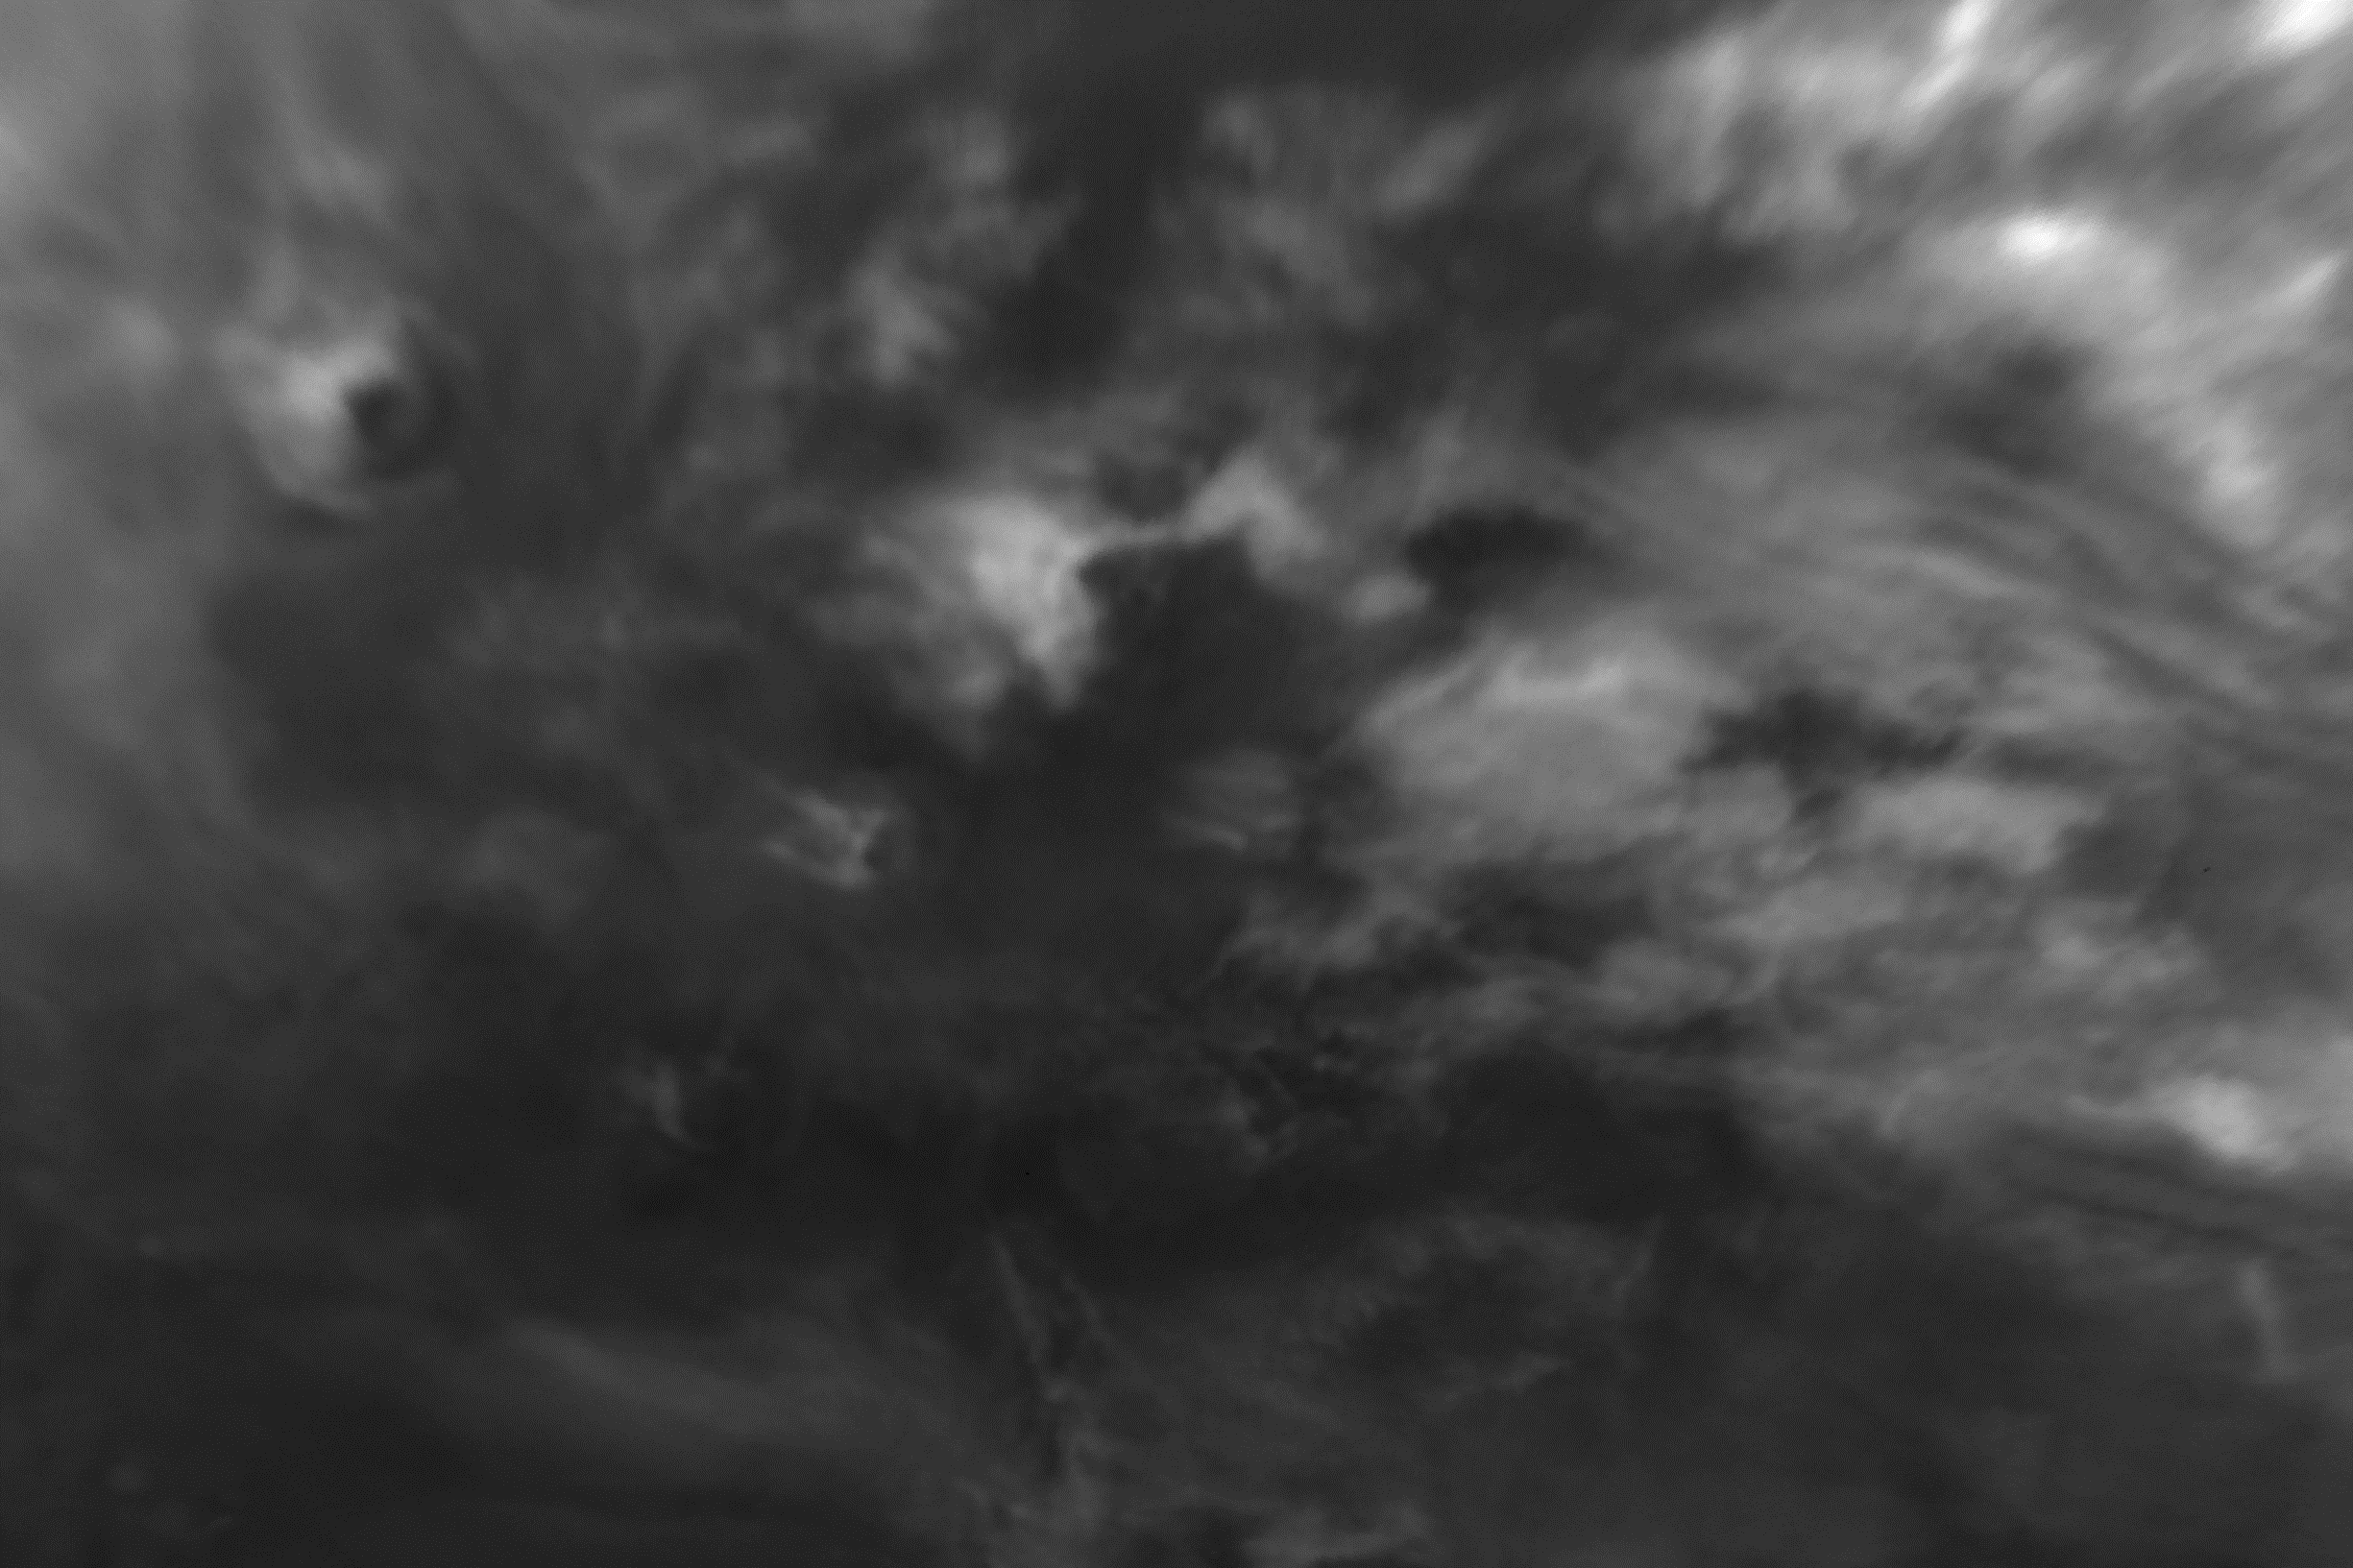
\includegraphics[width=0.8\textwidth]{fig_10.png}
    \caption{First cropped image in set 1 - UTC: 22/11/2021 14:16:52 (Latitude: -27.5° to 35.0°, Longitude: -148.75° to -55.0°), range in kilometers: approx. 5546 x 3697}
\end{figure}
\FloatBarrier
\begin{figure}[h!]
    \centering
    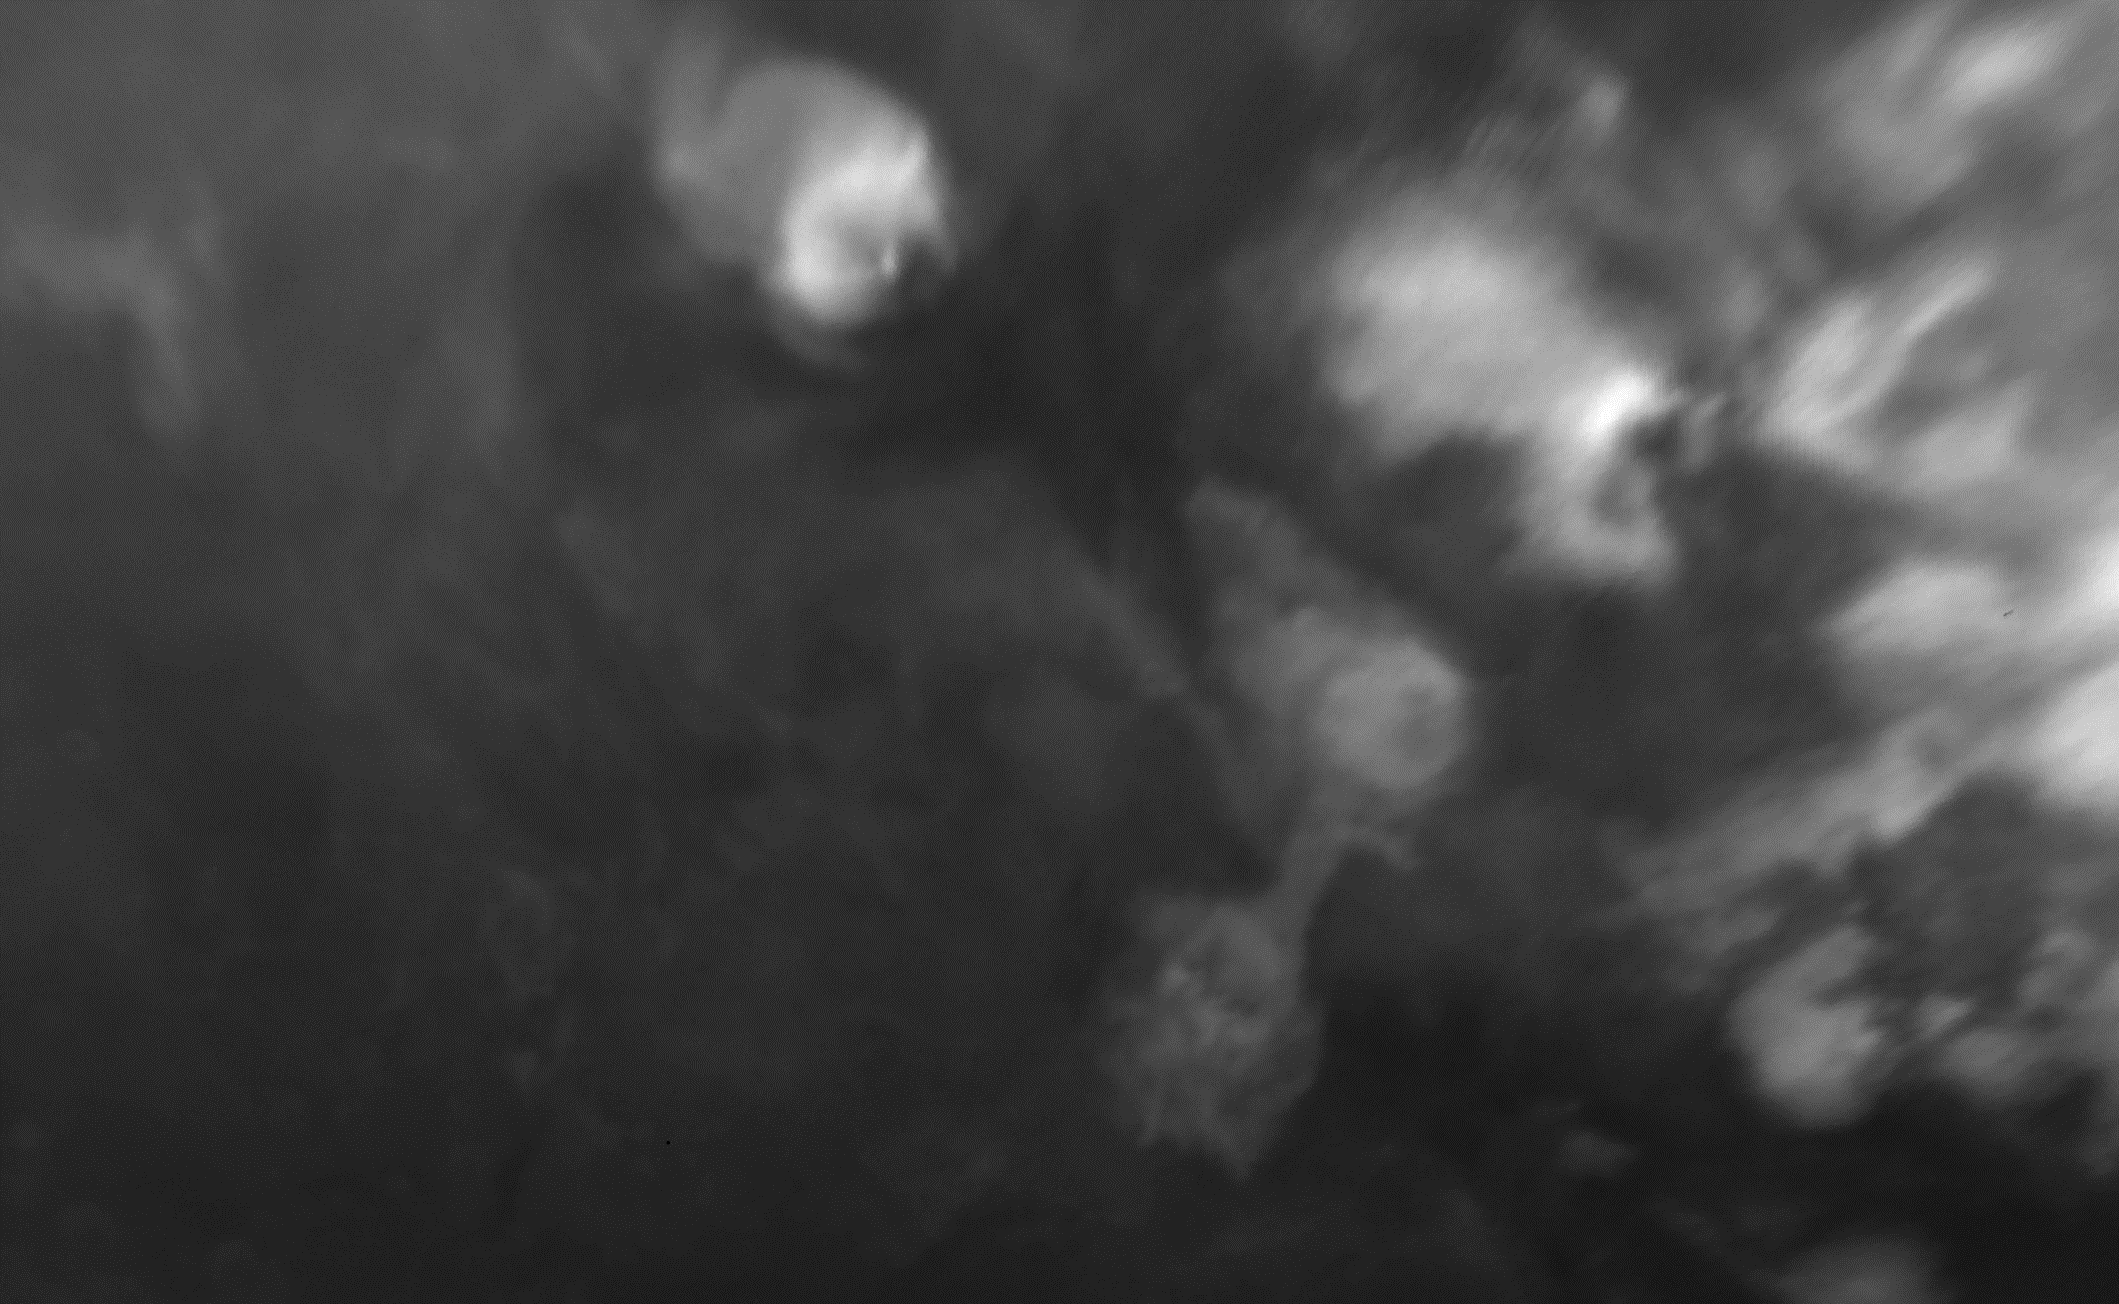
\includegraphics[width=0.8\textwidth]{fig_11.png}
    \caption{First cropped image in set 2 - UTC: 04/12/2021 00:31:53 (Latitude: -21.25° to 28.75°, Longitude: -167.5° to -86.25°), range in kilometers: approx. 4807 x 2958}
\end{figure}
\FloatBarrier
\begin{figure}[h!]
    \centering
    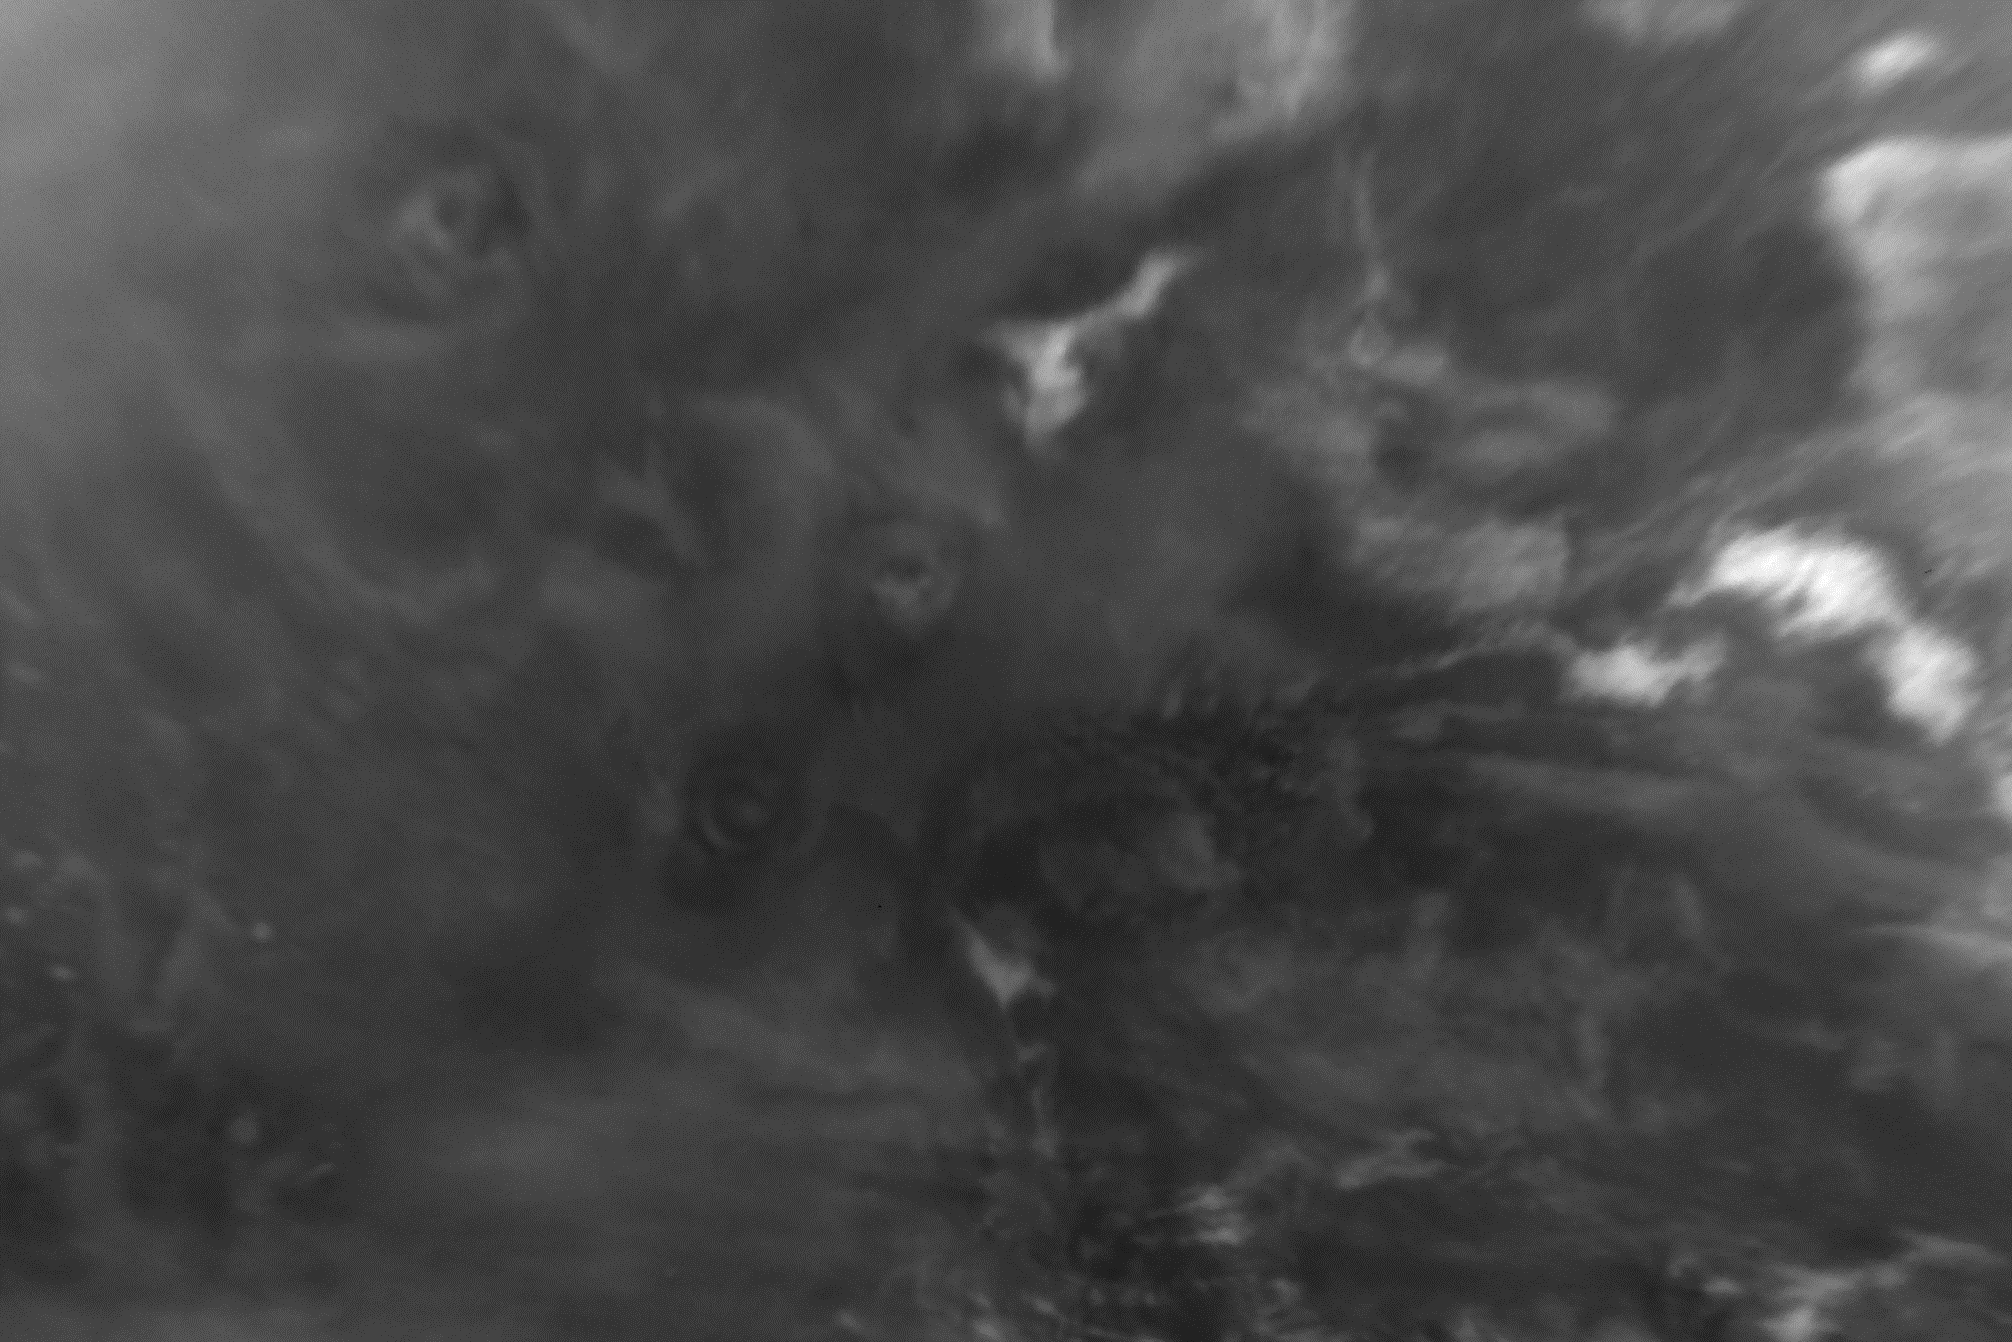
\includegraphics[width=0.8\textwidth]{fig_12.png}
    \caption{First cropped image in set 3 - UTC: 24/12/2021 10:30:07 (Latitude: -33.75° to 28.75°, Longitude: -155.0° to -61.25°), range in kilometers: approx. 5546 x 3697}
\end{figure}
\FloatBarrier
\begin{figure}[h!]
    \centering
    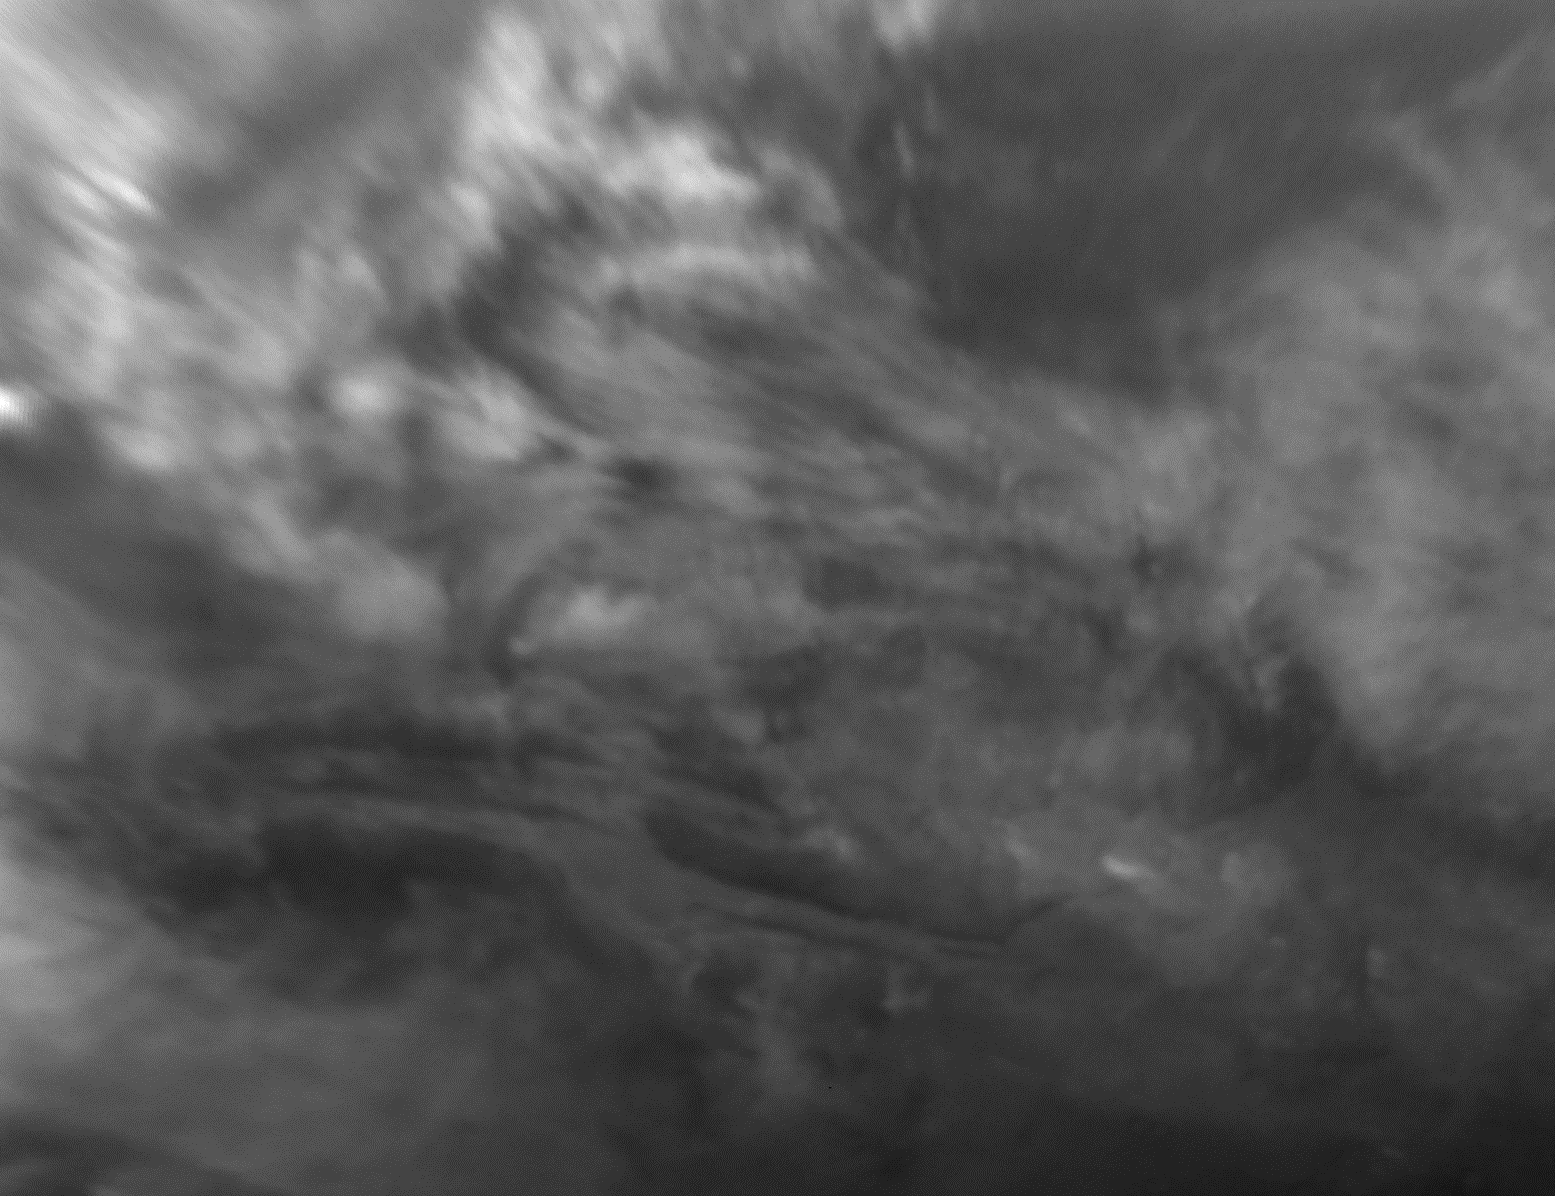
\includegraphics[width=0.6\textwidth]{fig_13.png}
    \caption{First cropped image in set 4 - UTC: 23/10/2023 05:40:13 (Latitude: -27.5° to 35.0°, Longitude: -105.0° to -23.75°), range in kilometers: approx. 4807 x 3697}
\end{figure}
\FloatBarrier
\begin{figure}[h!]
    \centering
    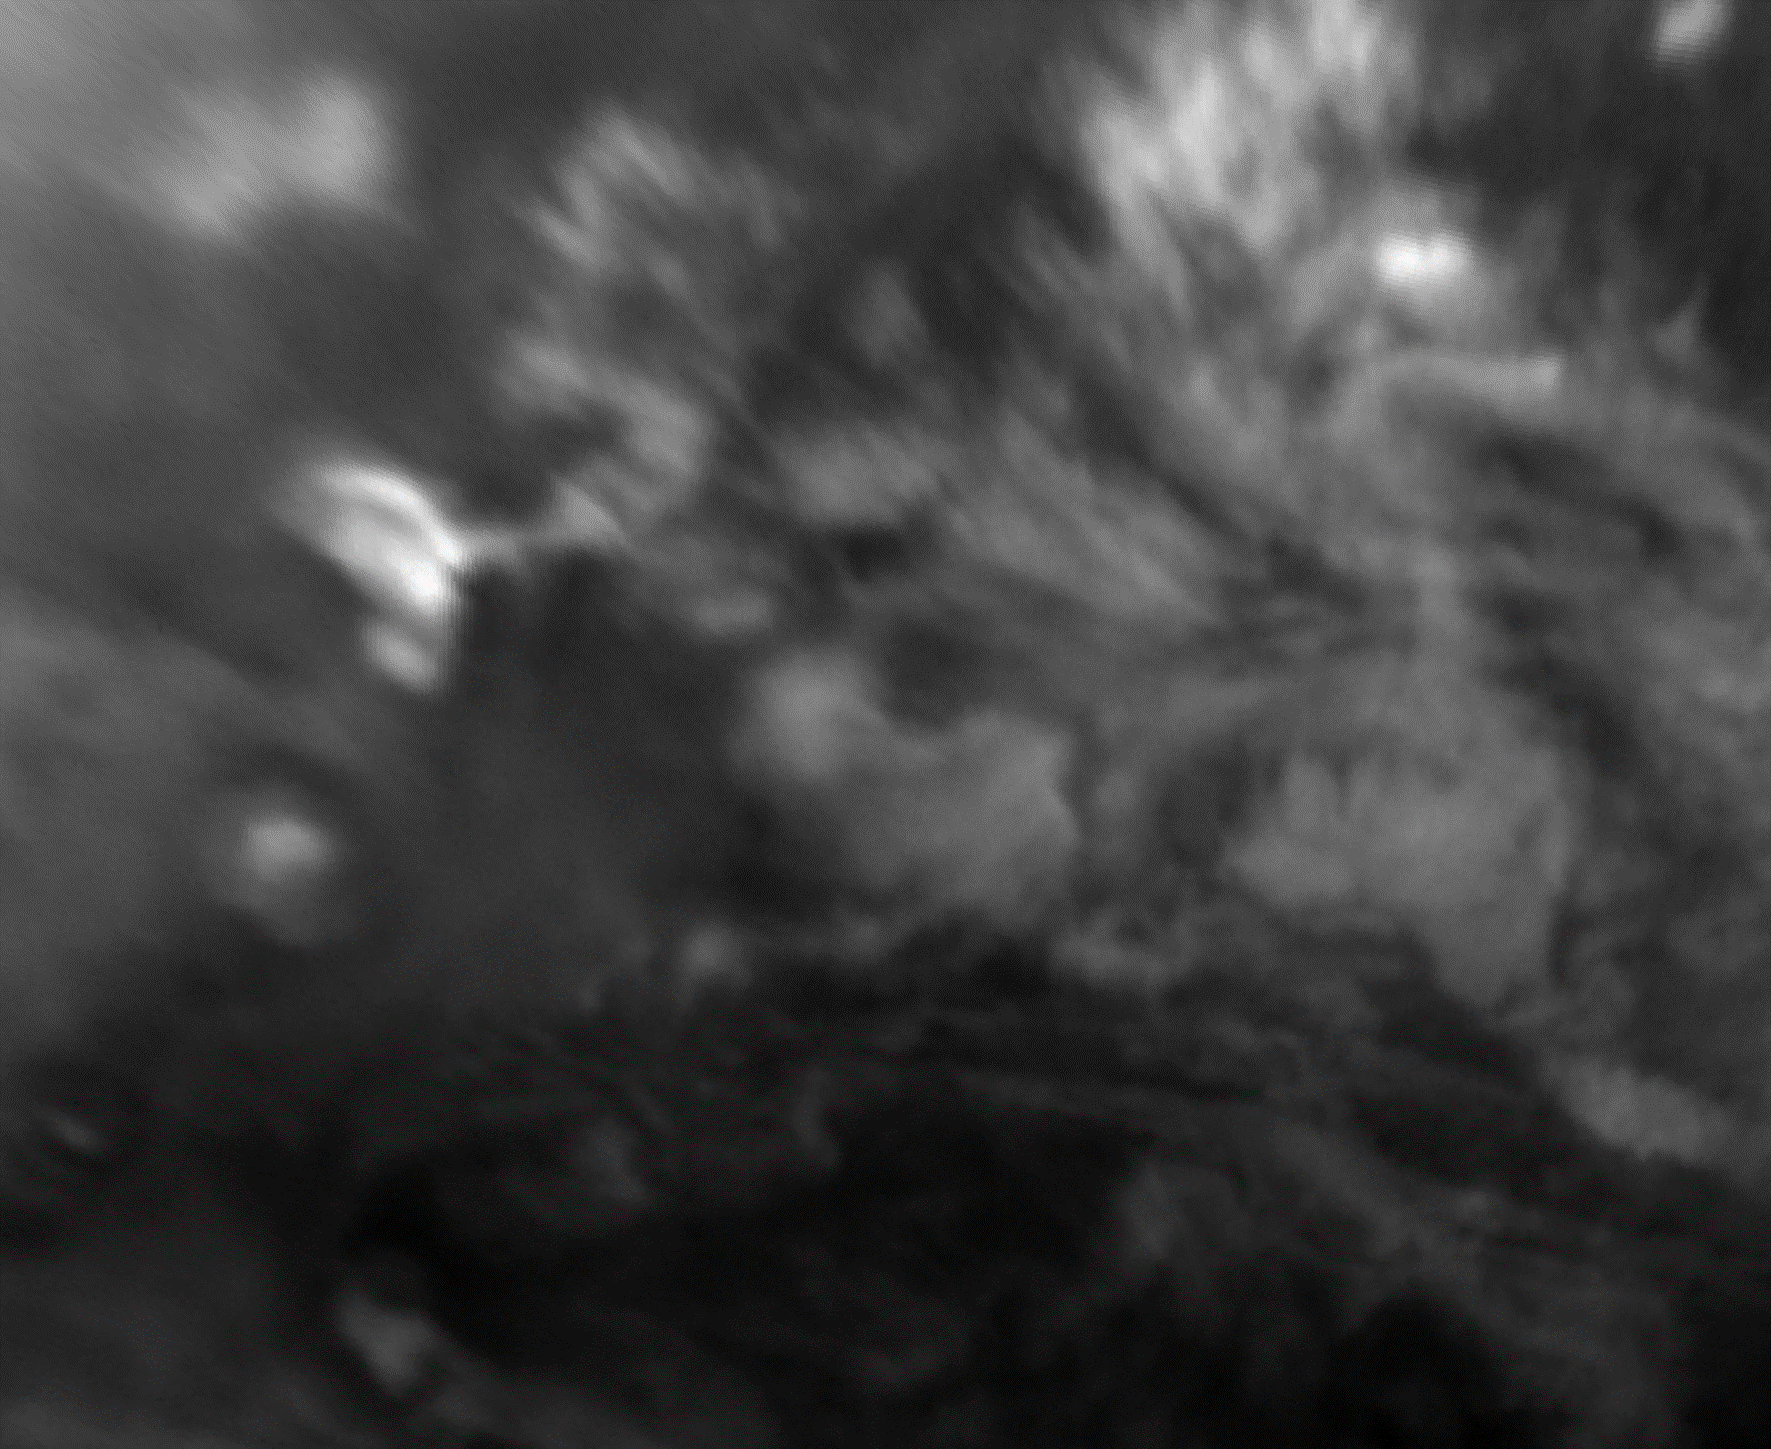
\includegraphics[width=0.6\textwidth]{fig_14.png}
    \caption{First cropped image in set 5 - UTC: 23/10/2023 08:18:33 (Latitude: -21.25° to 35.0°, Longitude: -123.75° to -55.0°), range in kilometers: approx. 4067 x 3328}
\end{figure}
\FloatBarrier
\begin{figure}[h!]
    \centering
    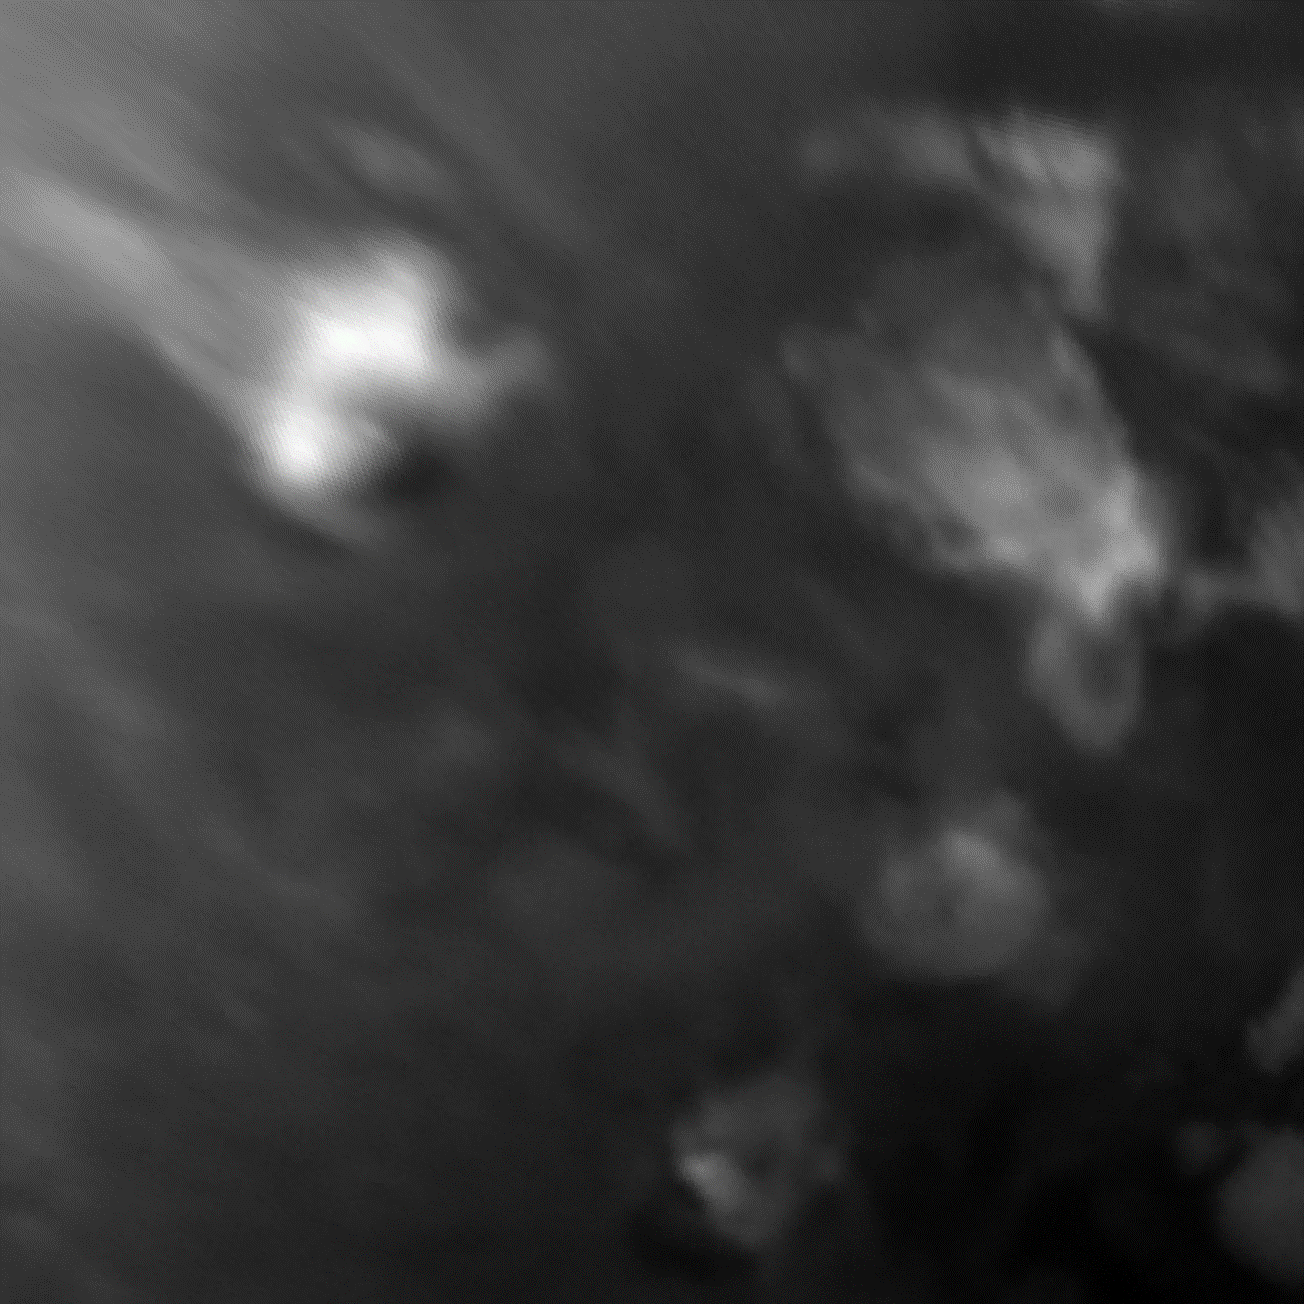
\includegraphics[width=0.6\textwidth]{fig_15.png}
    \caption{First cropped image in set 6 - UTC: 23/10/2023 10:56:50 (Latitude: -15.0° to 35.0°, Longitude: -148.75° to -98.75°), range in kilometers: approx. 2958 x 2958}
\end{figure}
\FloatBarrier
An overview of the first images from each sequence is displayed in Figures 2.9 through 2.14.
Based on visual observation, the images appear quite dark. This darkness may result from various factors, such as the scarcity of clouds in darker areas, differences in solar illumination, and the presence of cloud shadows.
There are noticeable brightness inconsistencies within the sequences and the clouds are spread out over larger regions with occasional brighter hot-spots. 
\FloatBarrier
\begin{figure}[h!]
    \centering
    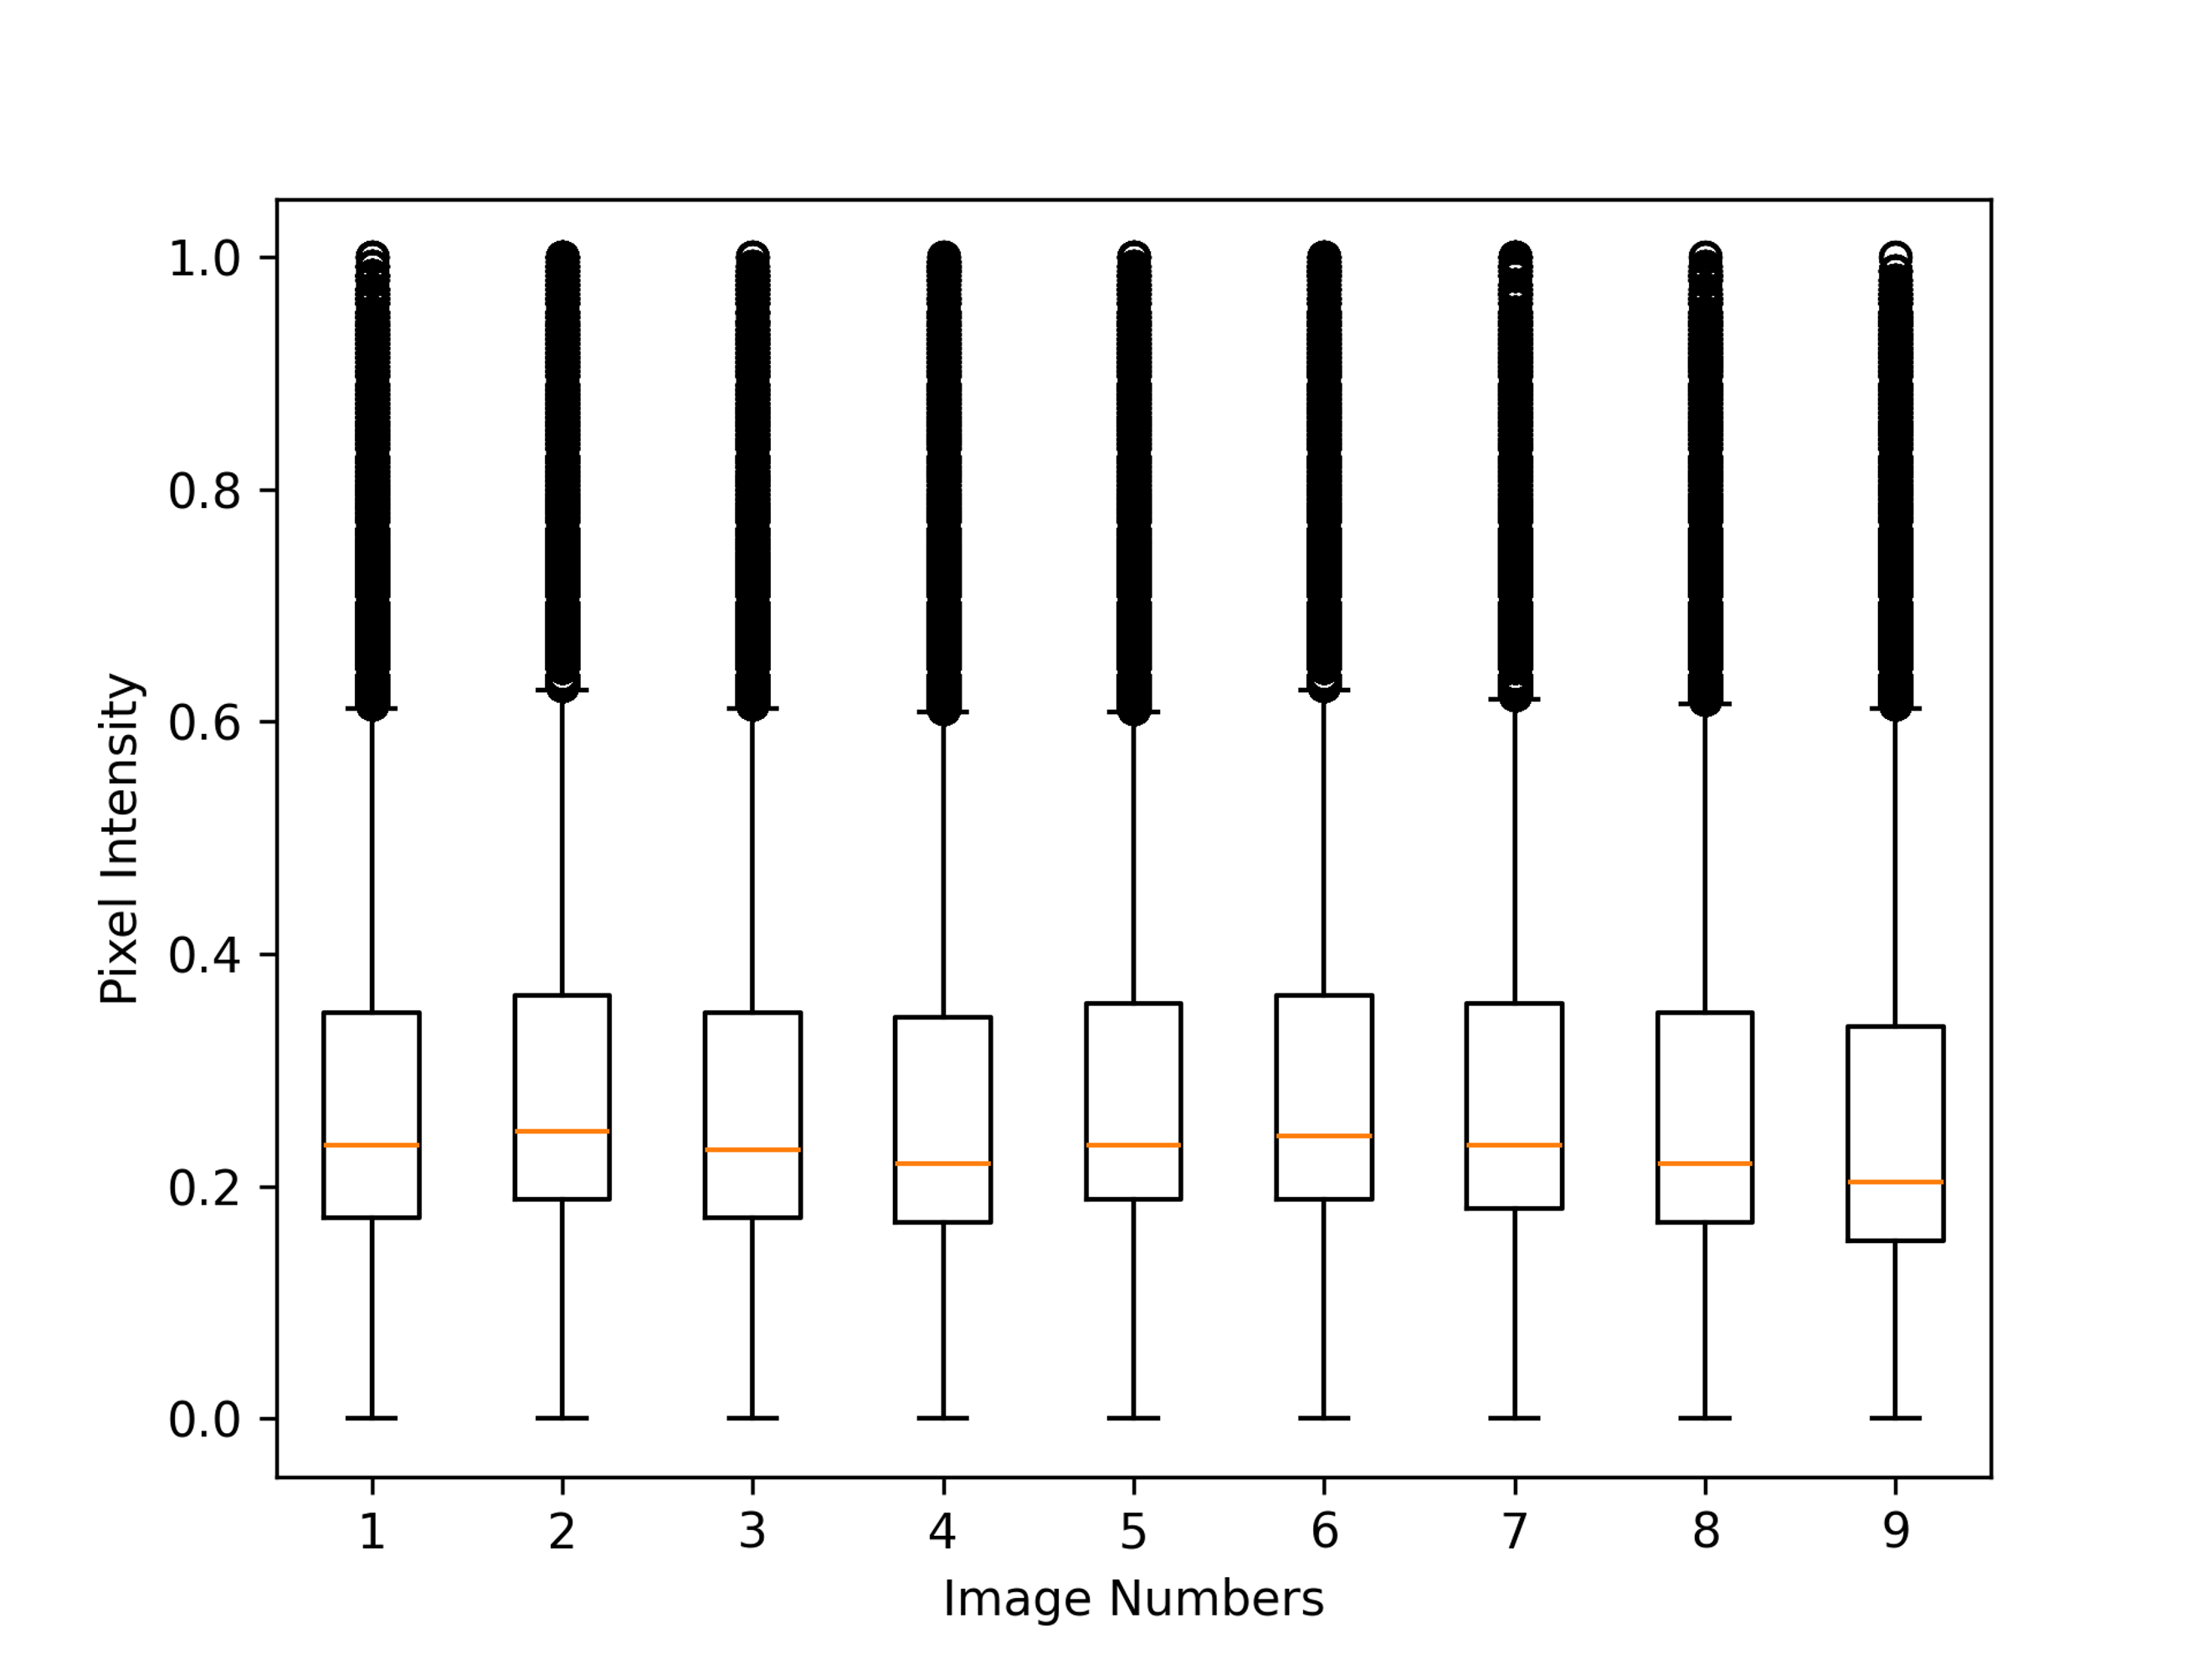
\includegraphics[width=0.8\textwidth]{fig_16.png}
    \caption{Box plot of the pixel data of each image in the sequence from UTC: 22/11/2021 14:16:52 - 14:56:52. The red lines are the medians and the upper parts, which appear like thick black lines, are the fliers, which are shown as black dots. }
\end{figure}
\FloatBarrier
\begin{figure}[h!]
    \centering
    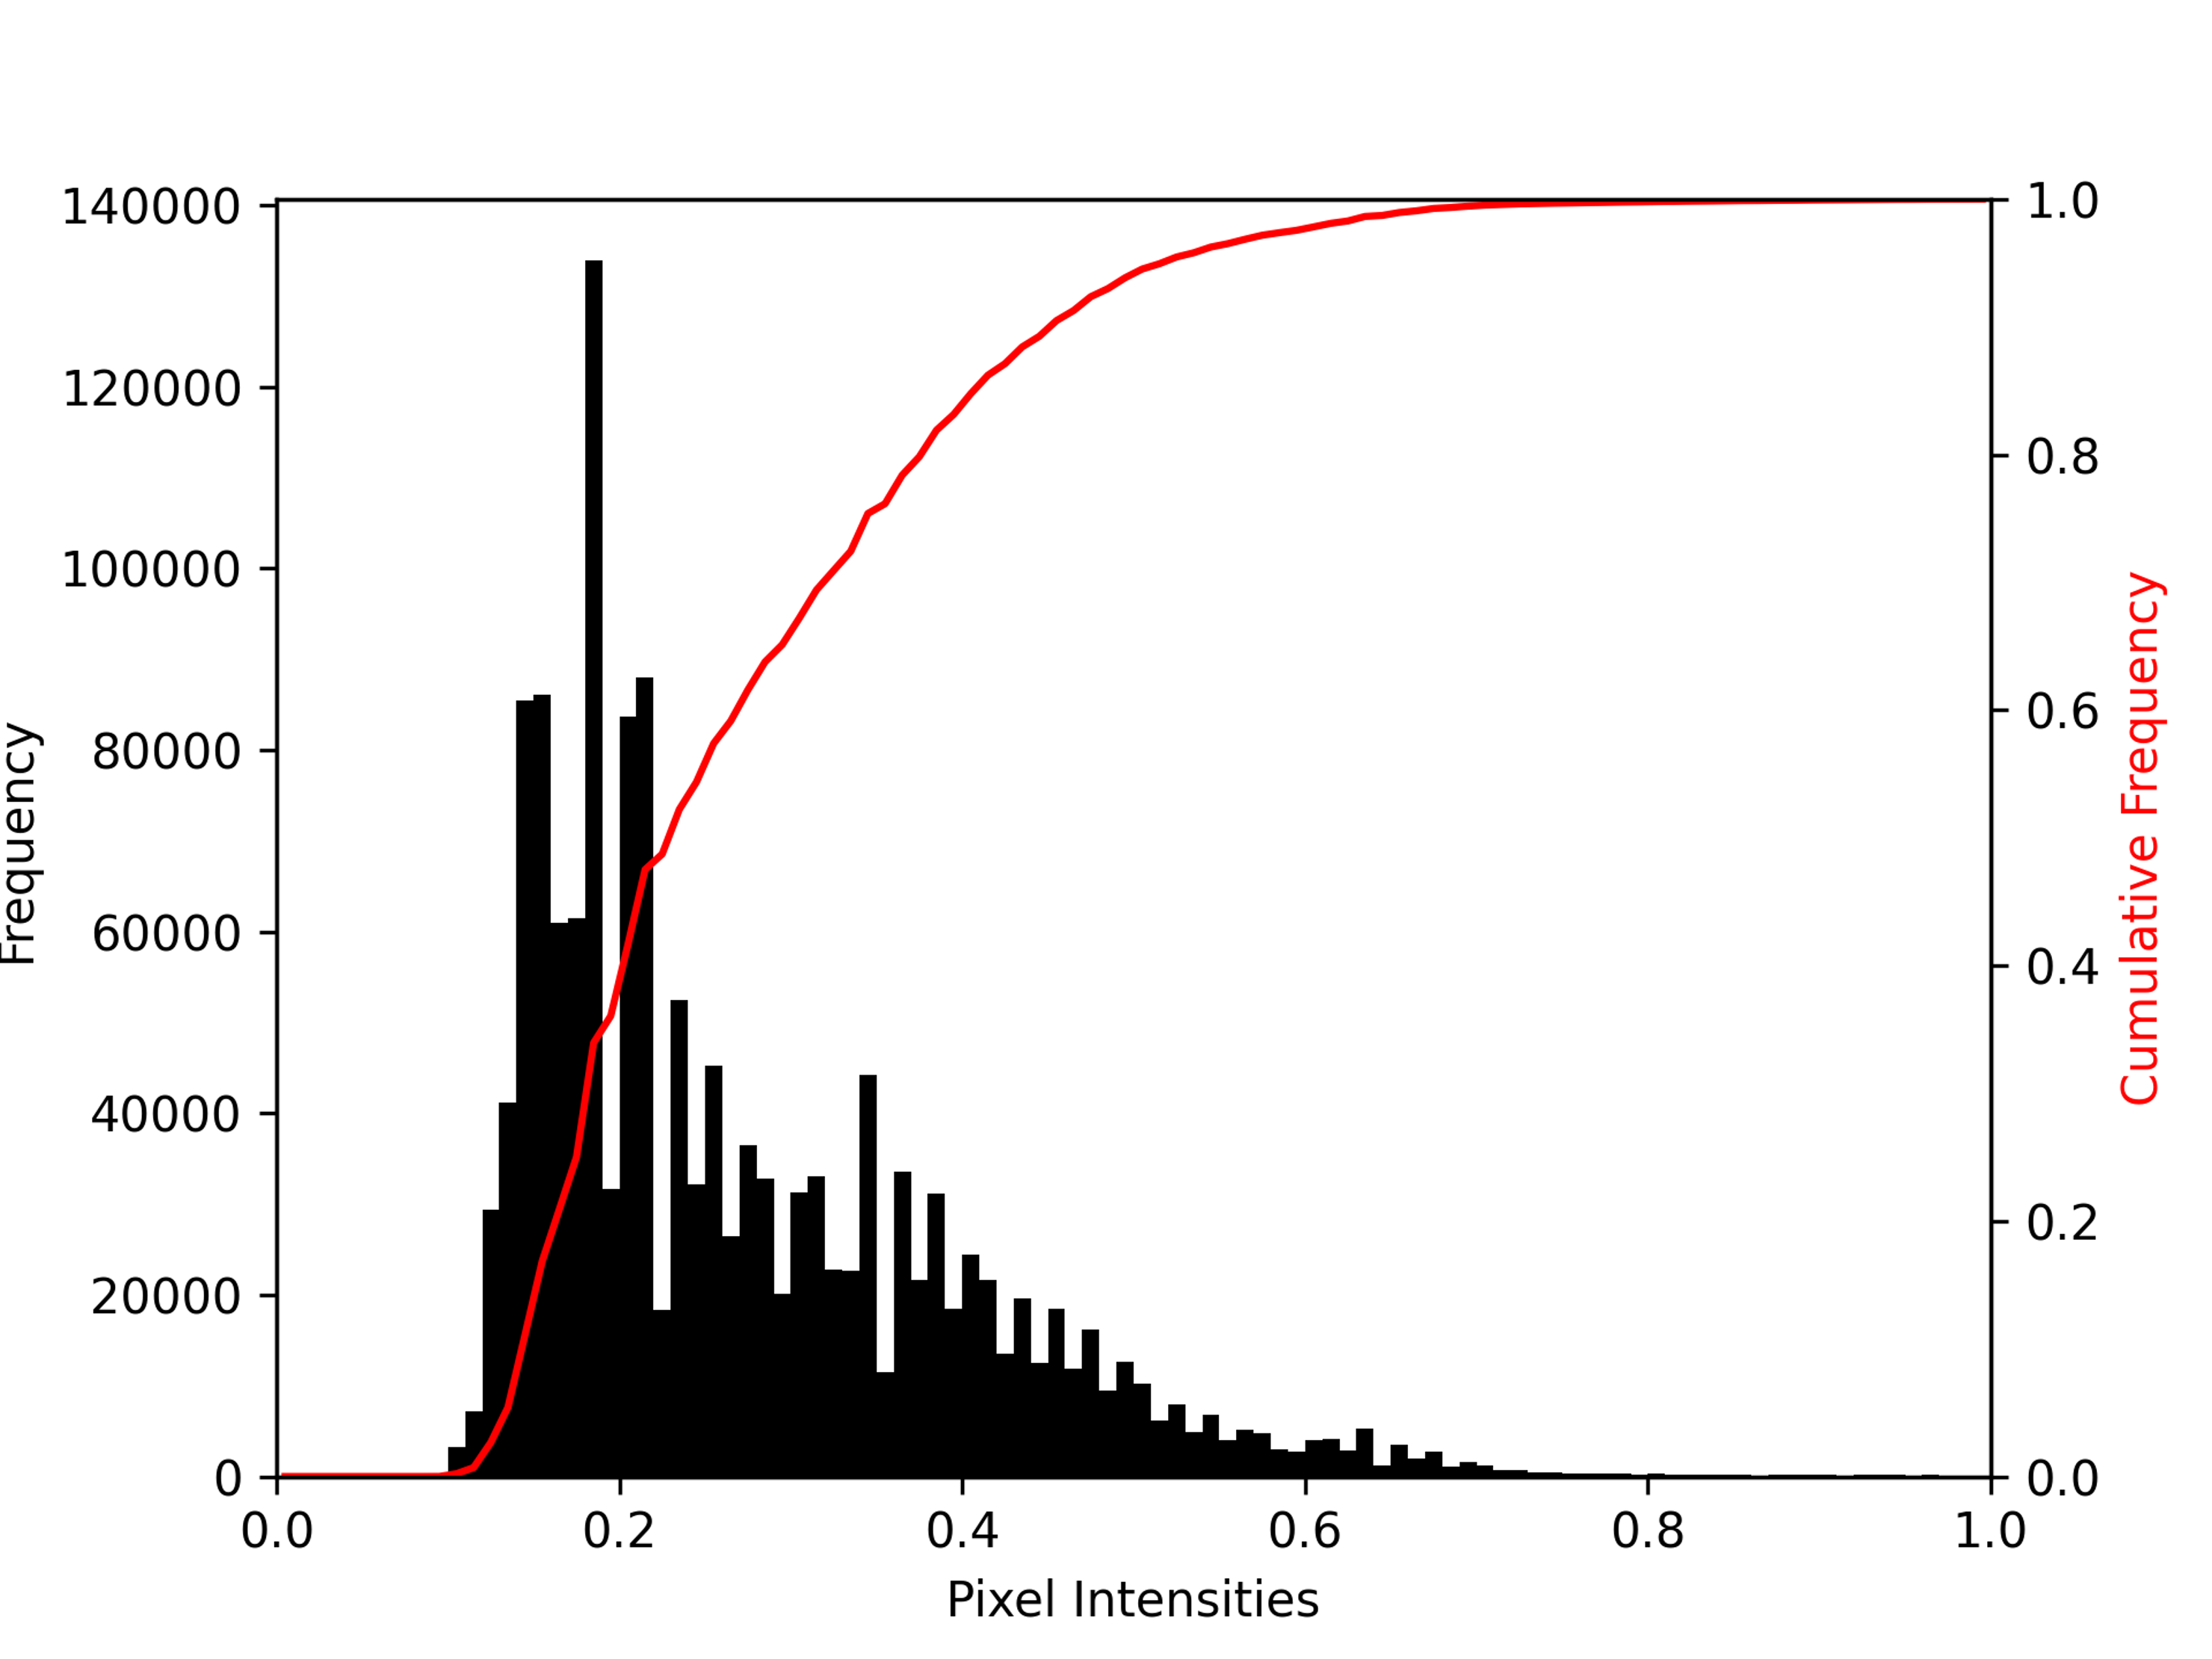
\includegraphics[width=0.8\textwidth]{fig_17.png}
    \caption{Histogram and CDF from UTC: 22/11/2021 14:16:52.}
\end{figure}
\FloatBarrier
The contrast of the images tends to be on the lower side. Box plots for each sequence (as shown in Figure 2.15) confirm the visual observations. Pixel data, up to the third quartile, is concentrated in low-to-medium intensities, resulting in dark images. However, some data points are scattered across higher intensities. Additionally, the median values in the box plots indicate variations in brightness levels within each sequence. Pixel Intensity histograms (see Figure 2.16), plotted with 100 bins, show a positive skewness across all image sequences, reflecting the fewer lighter intensities. The cumulative distribution function (CDF), plotted alongside the histogram, illustrates the rate of increase in intensities across the lower-to-medium intensity range.

After analysing the image data in the spatial domain, the fourier transform was computed to obtain details about the frequency domain, revealing cloudy features in higher frequencies (see Figure 2.17). 
\FloatBarrier
\begin{figure}[h!]
    \centering
    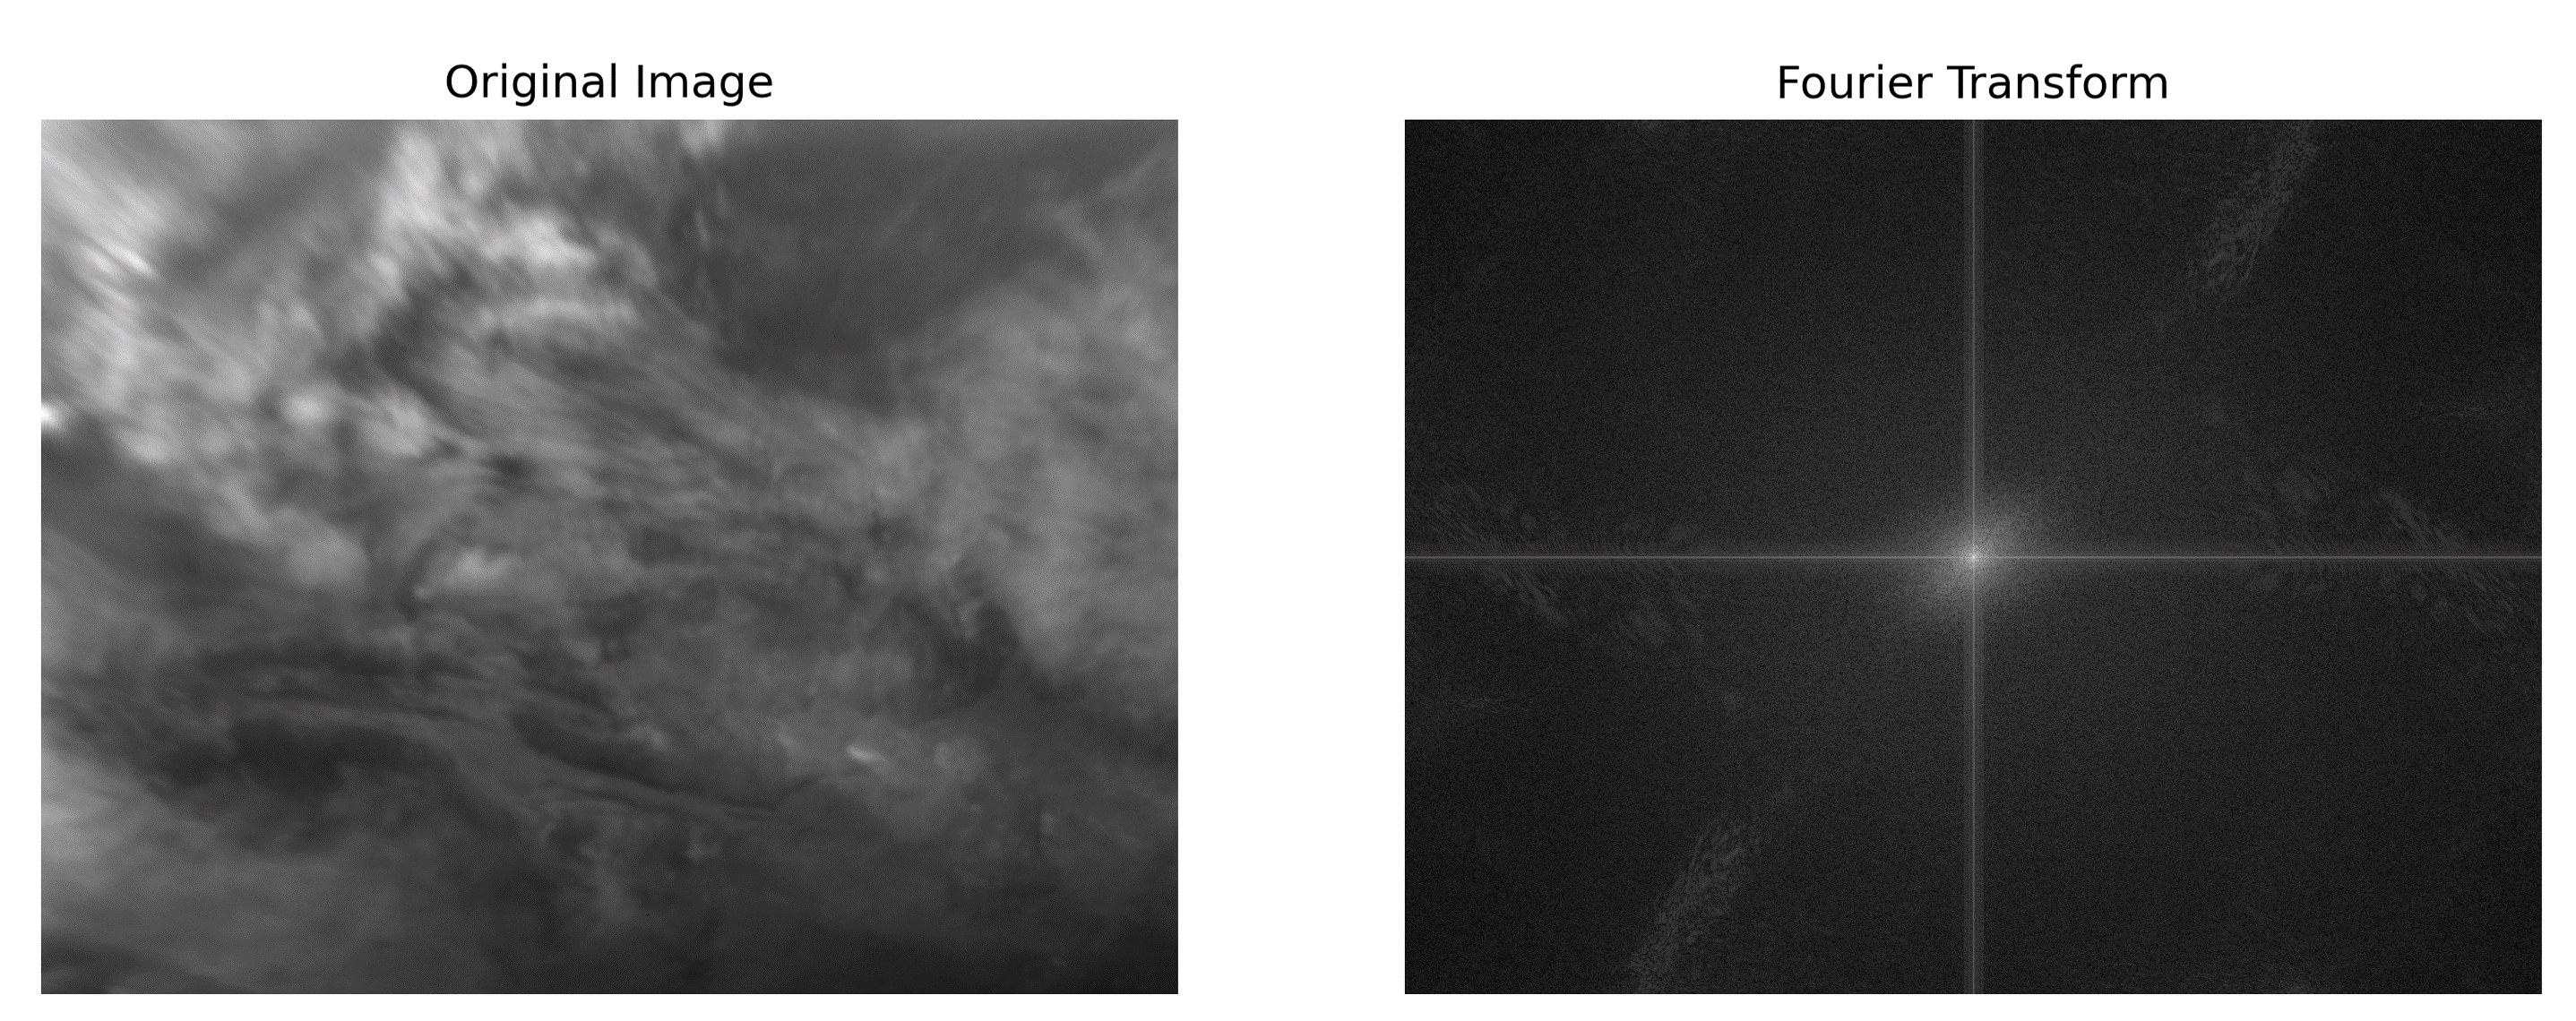
\includegraphics[width=1\textwidth]{fig_18.png}
    \caption{Magnitude spectrum of image from UTC: 23/10/2023 05:40:13.}
\end{figure}
\FloatBarrier
To investigate these features, a high-pass filter with a cut-off radius of 40 pixels was applied (see Figure 2.18), which removes lower-frequency components, highlighting the higher-frequency details. Subsequently, the square-root of the pixels was computed to enhance the image's brightness.
\FloatBarrier
\begin{figure}[h!]
    \centering
    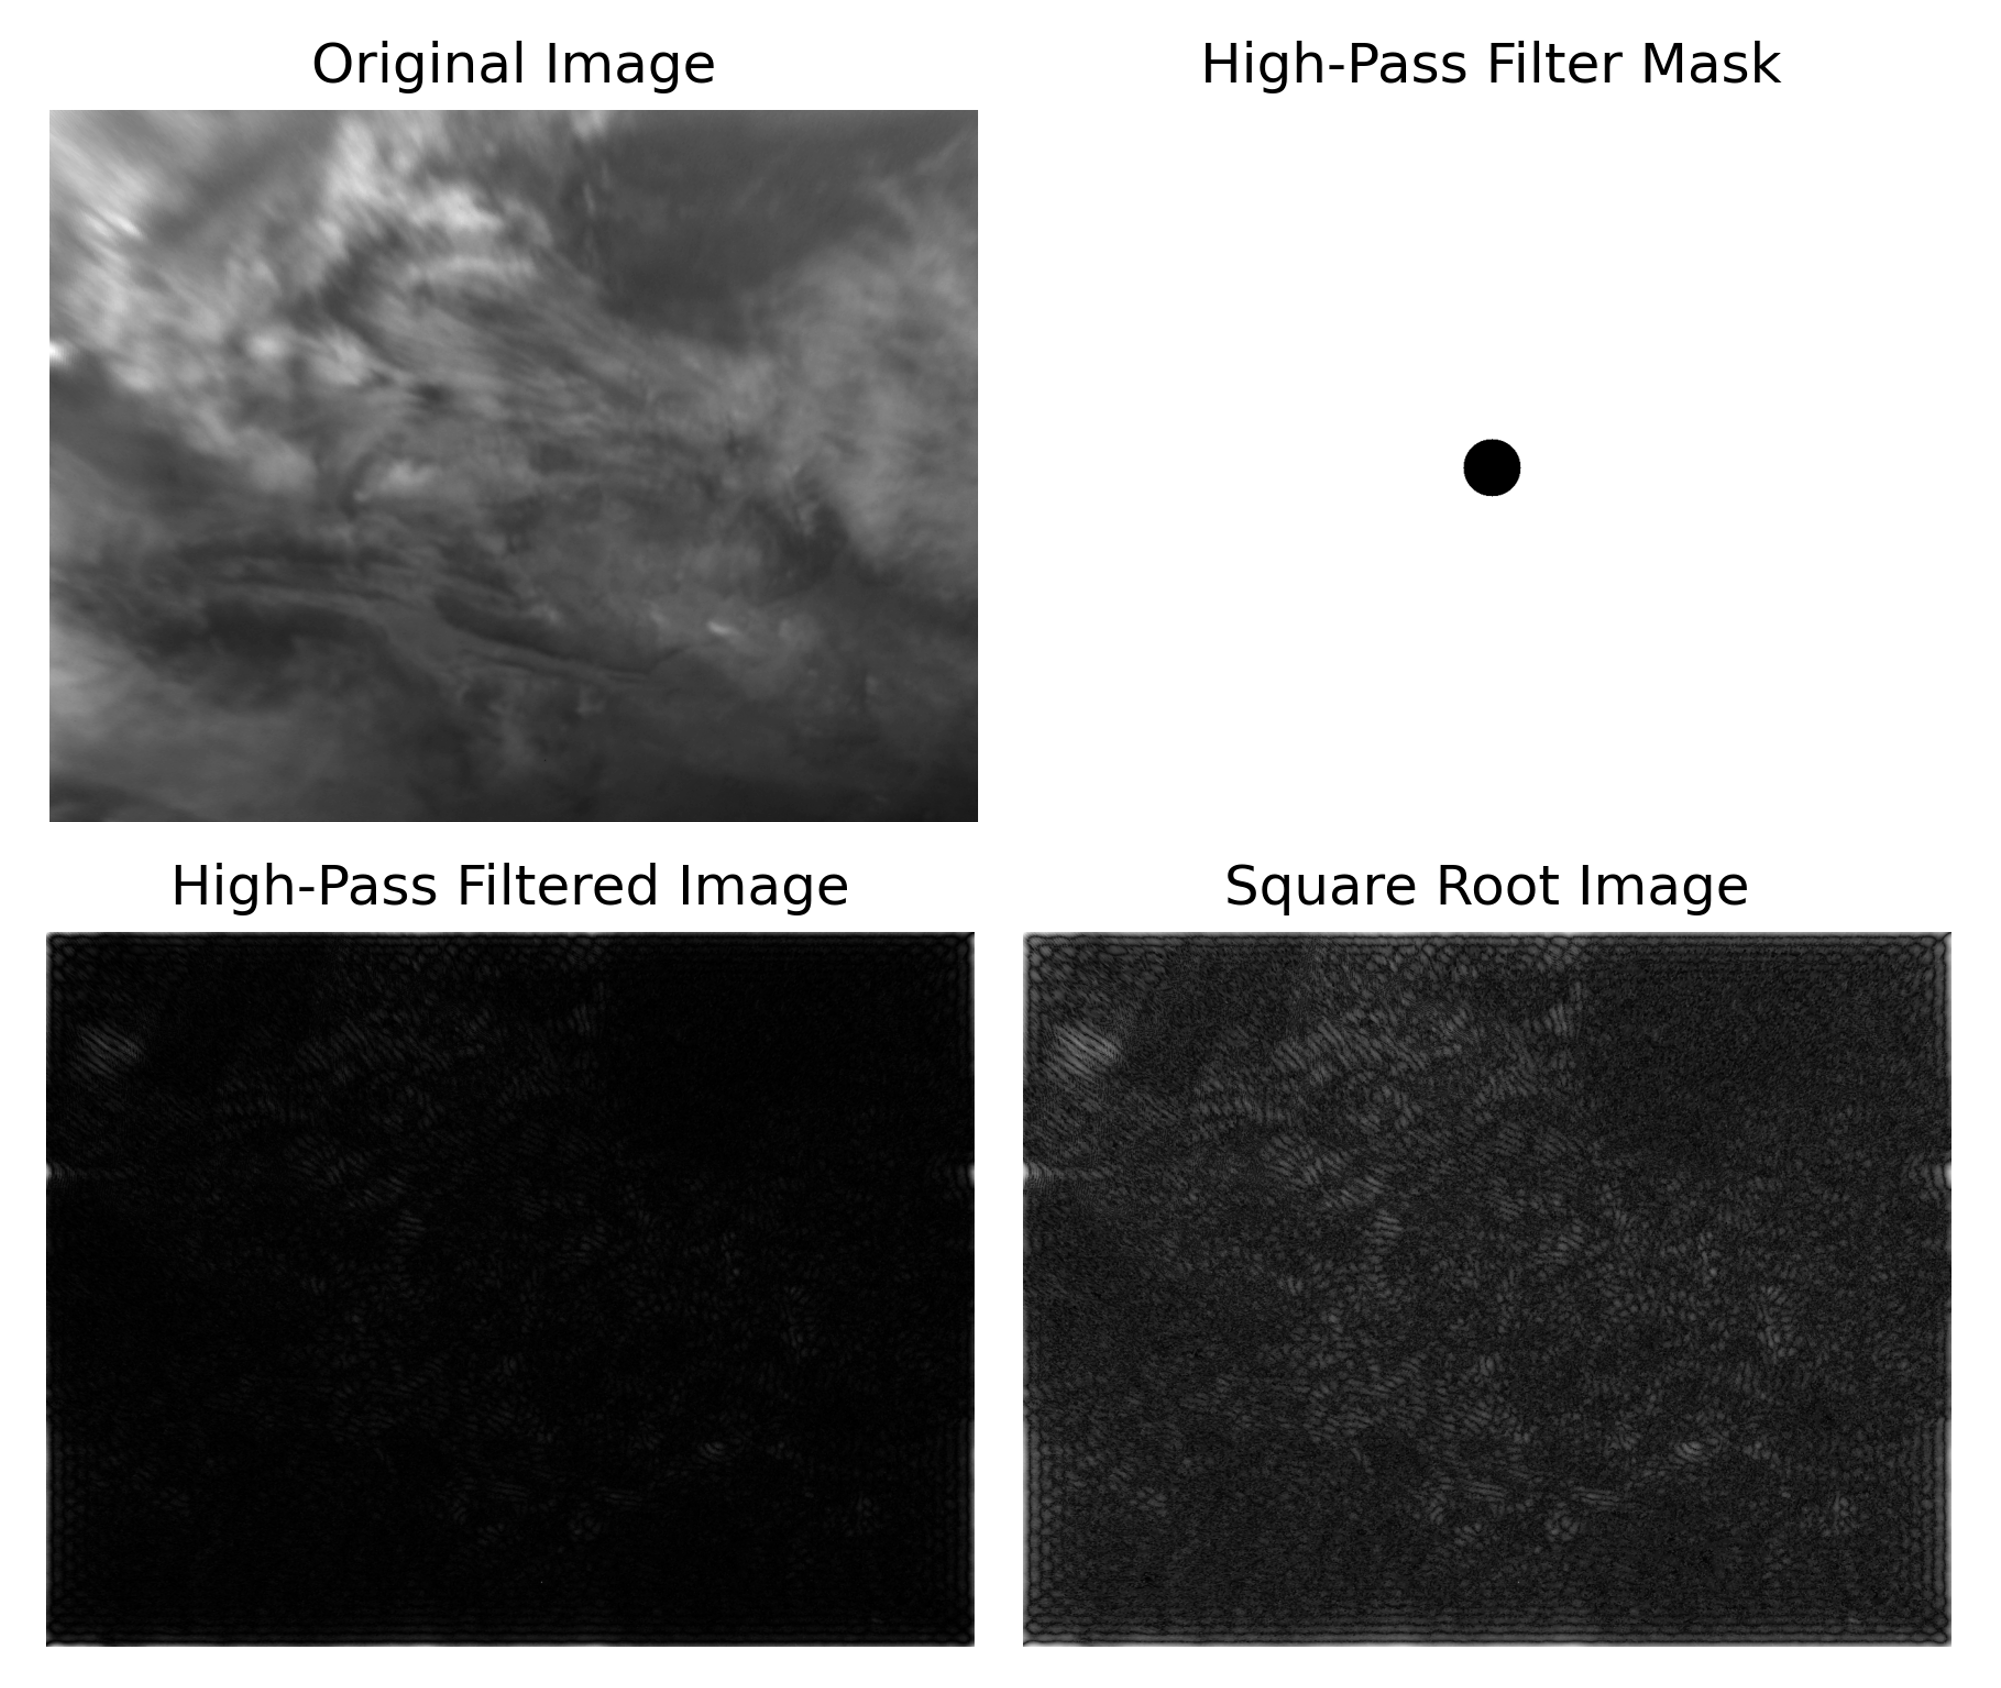
\includegraphics[width=1\textwidth]{fig_19.png}
    \caption{UTC: 23/10/2023 05:40:13 - overview of original image, high-pass filter mask, high-pass filtered image and square root image. The pixels of the high-pass filtered image were transformed using the square root to enhance contrast and improve visualization.}
\end{figure}
\FloatBarrier
The results indicate the presence of atmospheric waves. Increasing the cut-off radius in the high-pass filter highlights shorter wavelengths, while a lower cut-off radius brings out longer wavelengths. However, a cut-off radius that is too large, is not effective since the upper limit of the wavelength is constrained and a cut-off radius that is too small doesn't capture meaningful results either, possibly due to pixel resolution (see Figure A.1).

\chapter{Methods\label{chap:methods}}

Image processing and CIV analysis were conducted in self-written Python code using the following libraries: Astropy, Matplotlib, NumPy, Pandas, NetCDF4, and Skimage.

\section{Image Processing}

Since Cross-Correlation Image Velocimetry (CIV) relies on detecting moving features in image sequences, the aim is to enhance cloud visibility by improving image contrast. This approach is intended to make clouds more distinguishable and facilitate more accurate cloud tracking. To achieve this, four spatial domain image processing methods were selected for comparison: histogram matching, histogram equalization (HE), contrast limited adaptive histogram equalization (CLAHE), and sigmoid transformation. Other methods such as histogram slicing and stretching were avoided because they would have resulted in the loss of certain pixel intensities while the chosen methods preserve all data.

\subsection{Histogram Matching}

Given the slight variations in brightness observed among the image sequences, histogram matching, was applied. The goal was to achieve consistent brightness across all images within a sequence, thereby improving the similarity of pixel intensities for moving features and reducing the impact of variations in solar illumination.

Histogram matching is used to generate images, that have a specified histogram. It was implemented in this thesis using the skimage package in Python. The steps include the computation of the source image’s cumulative distribution function (CDF) and the target image’s CDF, which are used to determine a mapping function\cite{Gonzalez2018}. This function maps each intensity in the source image by finding the intensity in the target image that is closest to the corresponding value in the CDF of the source image. 

Since the CDF is derived from the PDF, the probability density function is given by\cite{Gonzalez2018}: 

\begin{equation}
p(r_k) = \frac{n_k}{N}
\end{equation}

where \( n_k\) is the amount of intensity values \( r_k \) and \(N\) the total number of pixels in the image, while \( p(r_k)\) is the probability of an intensity occurring at \( r_k \).

The cumulative distribution function is the running total of the probabilities from the PDF at each step, given by\cite{Gonzalez2018}: 

\begin{equation}
c(r_i) = \frac{1}{N} \sum_{j=0}^{r_i} n_j
\end{equation}

where \( r_i\) is the intensity level for which the CDF is calculated, \( n_j\) is the amount of intensities \( j\), \(N\) the total number of pixels and \(c(r_i)\) the cumulative probability up to the specified intensity \( r_i\). 

The pixel intensity mapping is given by\cite{Gonzalez2018}: 

\begin{equation}
s_i = \text{round} \left( \text{c}_{\text{target}}^{-1} \left( \text{c}_{\text{source}}(r_i) \right) \right)
\end{equation}

where \( s_i\) is the updated pixel intensity, \( r_i\) is the original intensity, \(\text{c}_{\text{target}}^{-1}\) is the inverse CDF of the target histogram, \(\text{c}_{\text{source}}(r_i)\) is the CDF of the source histogram at the intensity \( r_i\). The result is rounded to the nearest integer to enable mapping to the closest intensity, which wouldn't be possible with discrete values.  

For the selected sequences, the first image in each sequence served as the reference, and subsequent were adjusted based on the CDF of the reference. 
\FloatBarrier
\begin{figure}[h!] 
    \centering
    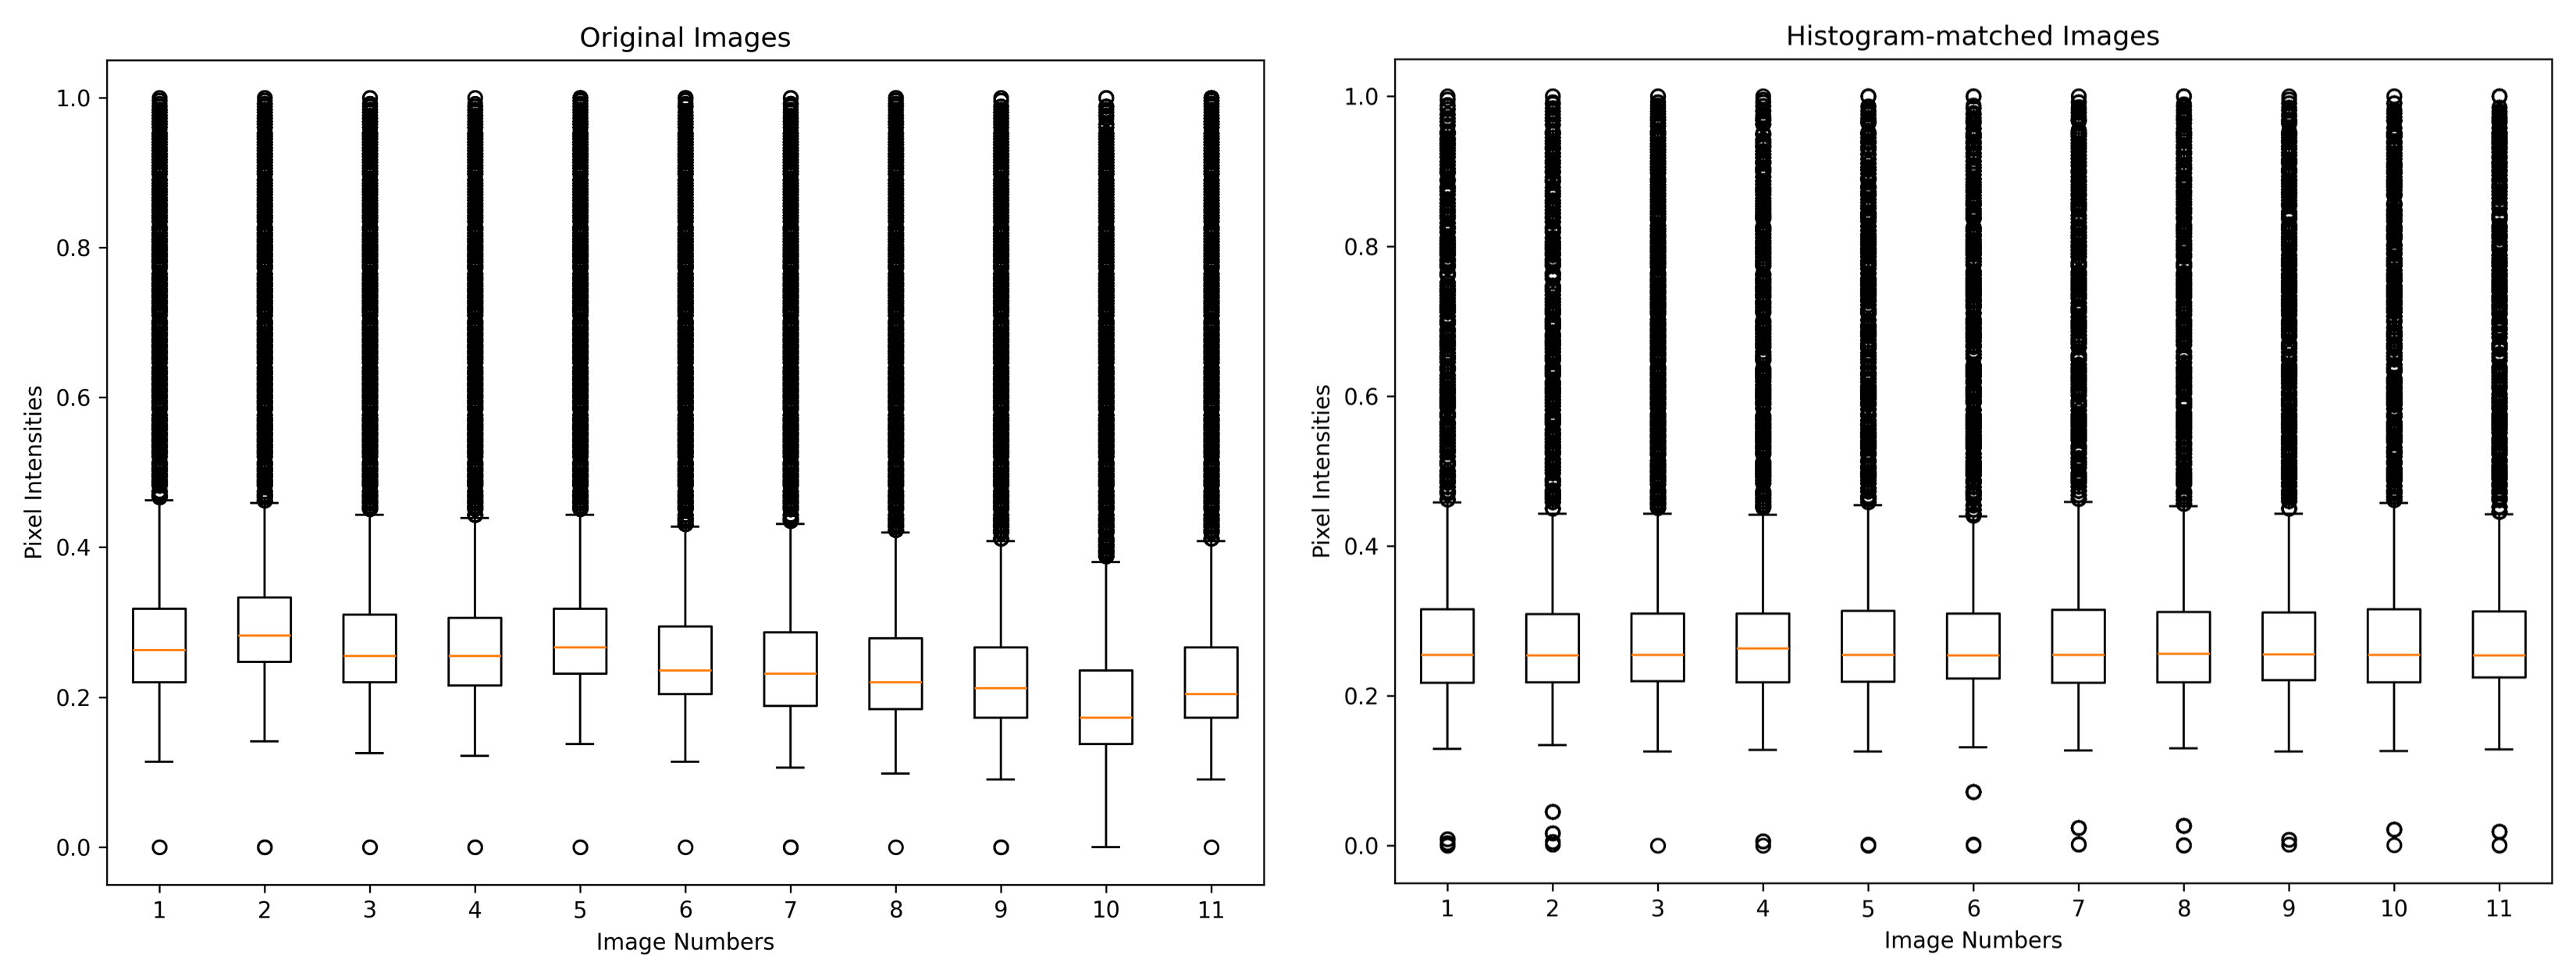
\includegraphics[width=1\textwidth]{fig_20.png}
    \caption{Box plot of the image sequence from UTC: 24/12/2021 10:30:07 - 11:20:06 before histogram matching on the left and after histogram matching on the right.}
\end{figure}
\FloatBarrier
The box plots (see Figure 3.1) and visual observation (see Figure 3.2) clearly indicate that the brightness levels within the sequences have become more consistent. 
\FloatBarrier
\begin{figure}[h!] 
    \centering
    \includegraphics[width=1\textwidth]{fig_21.png}
    \caption{Comparison of raw and histogram-matched images (UTC: 24/12/2021, 11:15:06 - 11:20:06). Upon closer inspection, the raw image on the left appears darker compared to the one on the right. The histogram-matched images below exhibit more consistent brightness levels.}
\end{figure}
\FloatBarrier
\subsection{Histogram Equalization}

Histogram equalization is widely used for contrast manipulation, readjusting the original histogram to produce a uniform population density of pixels\cite{Ghosh2013}. It makes both darker and lighter areas of the image more visible, improving the overall contrast.
The processing steps are similar to the ones for histogram matching. The only difference is the mapping function used, given by\cite{Gonzalez2018}: 

\begin{equation}
s_i = \text{round} \left((L-1) \cdot c(r_i) \right)
\end{equation}

where \( s_i\) is the updated intensity, \( L\) is the number of possible intensity levels and \( c(r_i)\) the CDF of the intensity at \( r_i\).
\FloatBarrier
\begin{figure}[h!] 
    \centering
    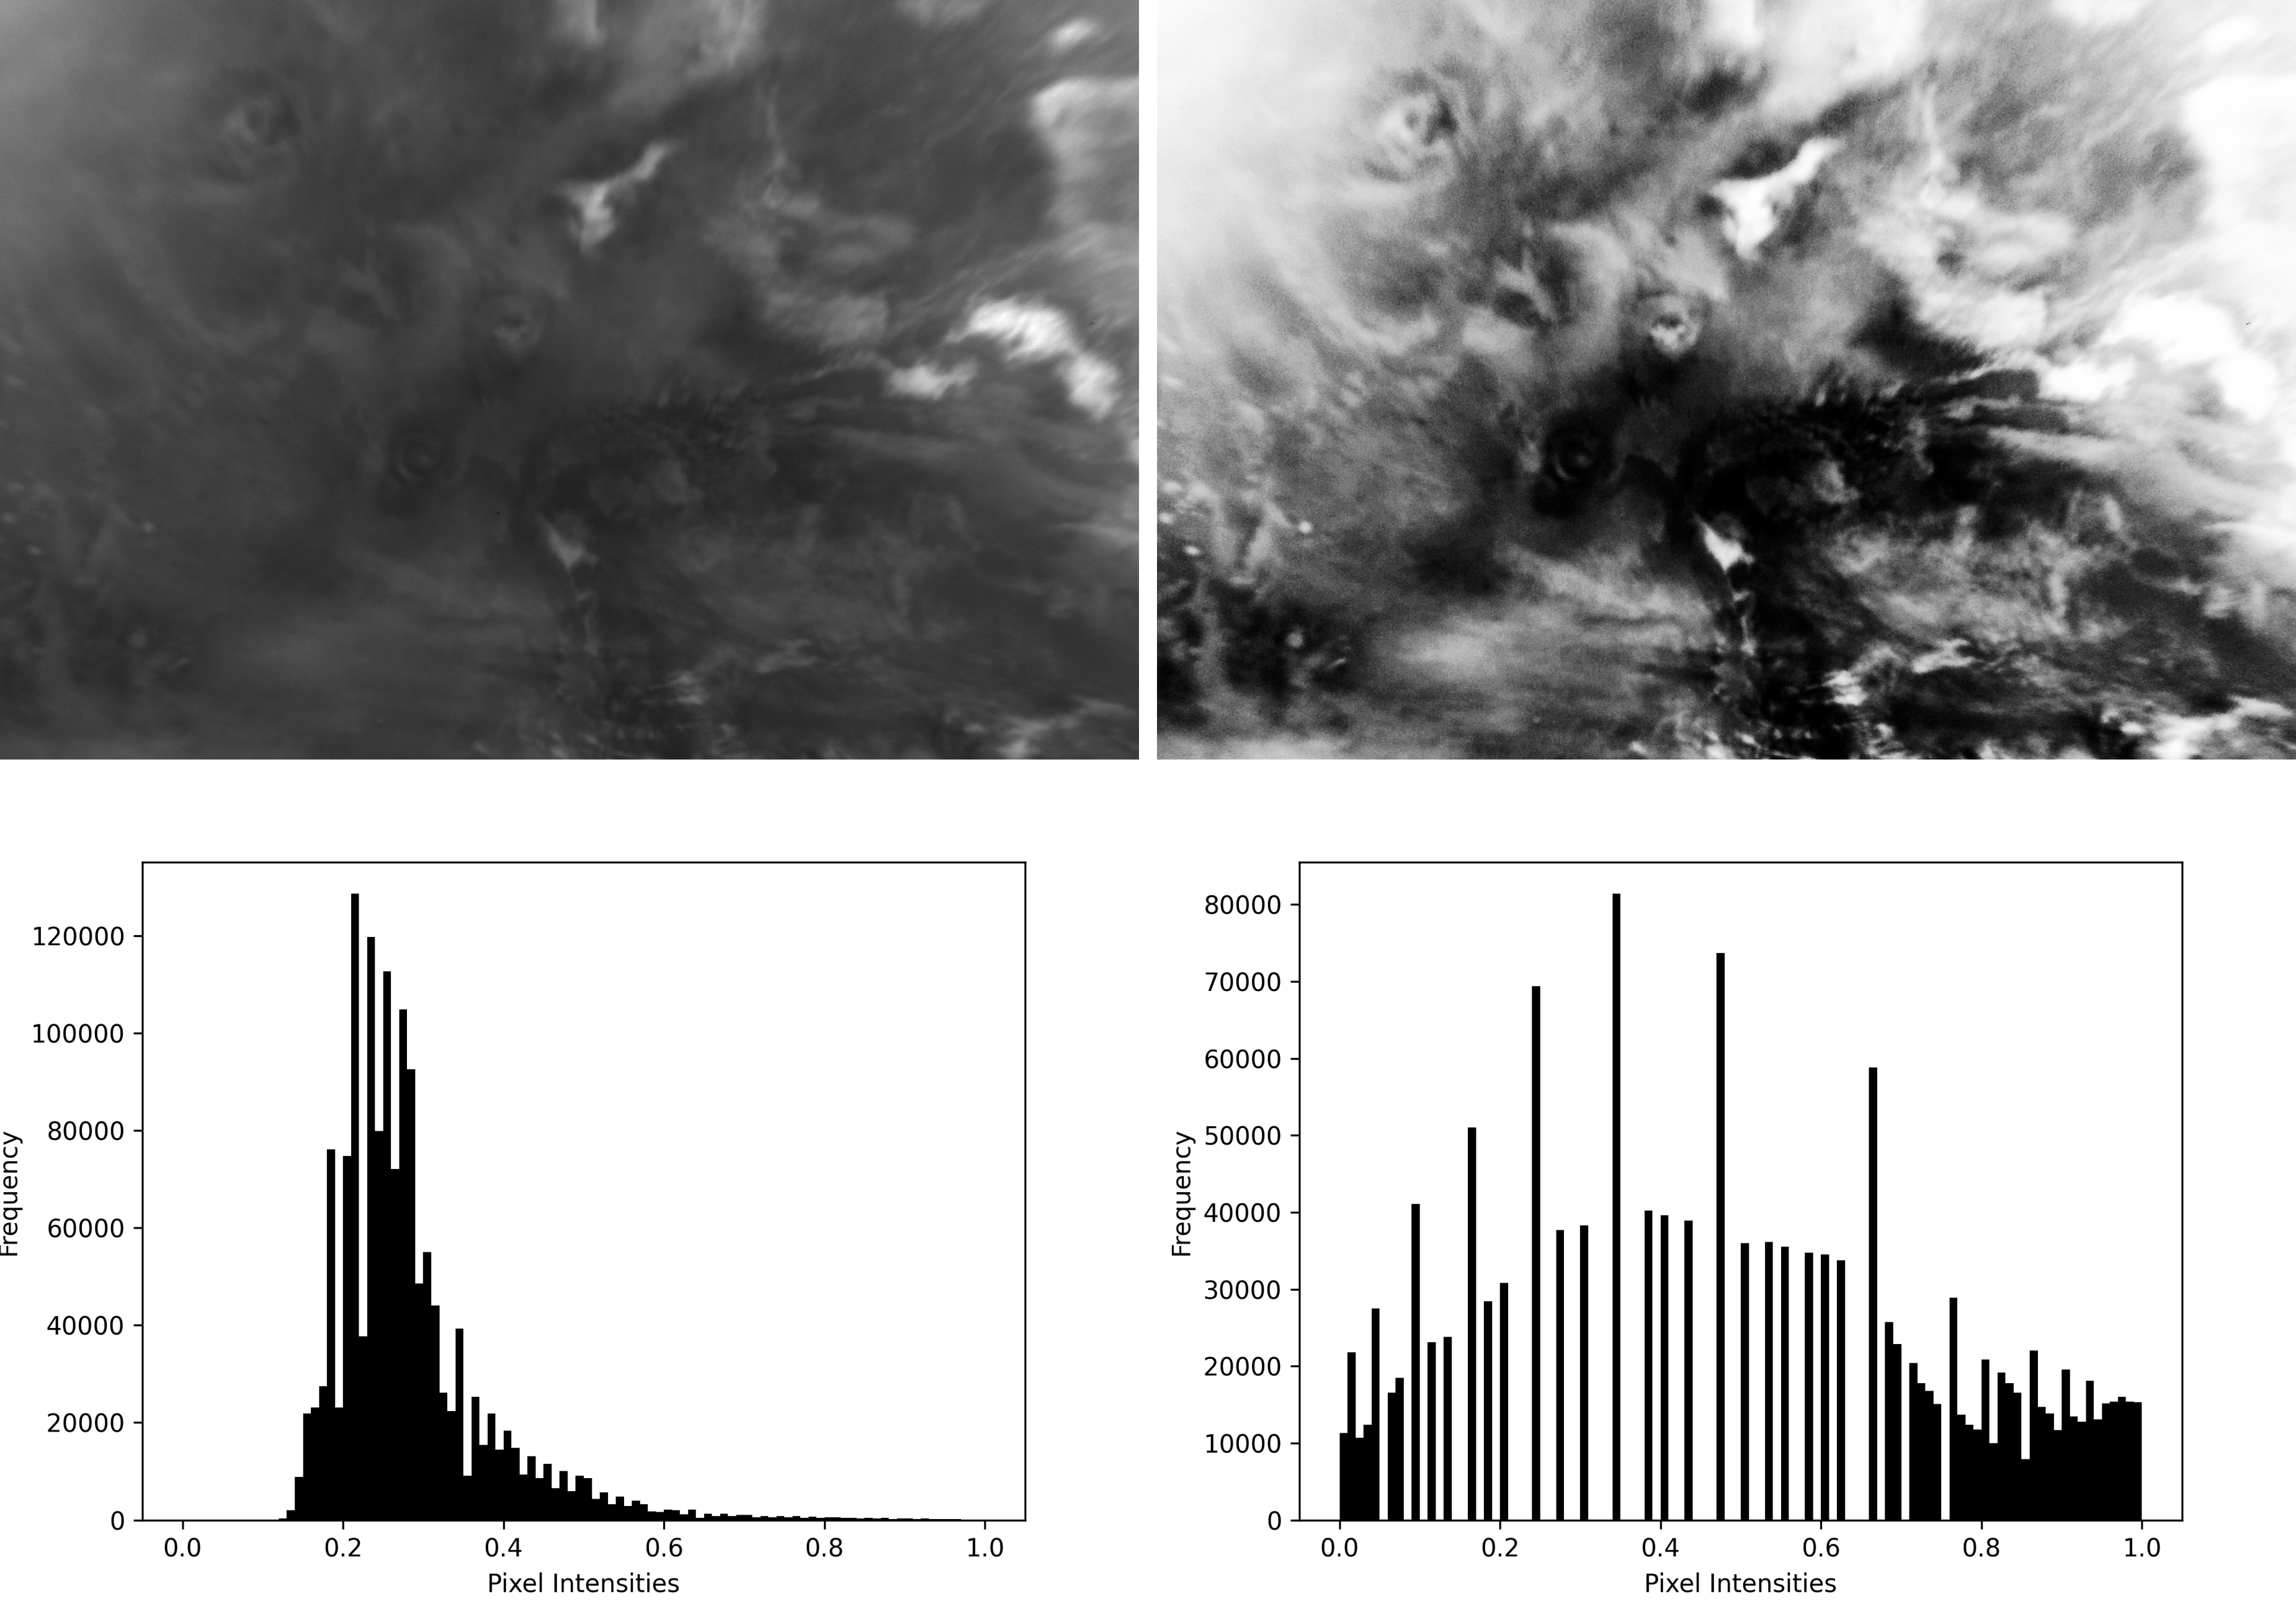
\includegraphics[width=1\textwidth]{fig_22.png}
    \caption{Comparison of raw and histogram-equalized image (UTC: 24/12/2021, 10:30:07). The original image including the intensity histogram are on the left, while the histogram-equalized image and the intensity histogram are on the right.}
\end{figure}
\FloatBarrier
The images exhibit higher contrast (as shown in Figure 3.3). Comparing the image histograms before and after HE, the pixel intensities are more evenly distributed across the intensity range.

\subsection{Contrast Limited Adaptive Histogram Equalization}

Adaptive Histogram Equalization is another technique for improving image contrast. It differs to histogram equalization in that for every pixel at position \( (i,j)\) in the image, the CDF is calculated for a filter window centered on that pixel, where the filter window size is defined before-hand and the window moves pixel-wise from left to right\cite{Haertinger2024}. It potentially maps a narrow range of input values to a wide range of output values if the window size encompasses a homogeneous image region. Histogram clipping, used in CLAHE, addresses this issue by reducing the amount of contrast enhancement by limiting histogram bins to a clip limit.

In this thesis, the clip limit was set to 0.1, hence intensity values in uniform regions of the image are not increased by more than 0.1. Thereby, the contrast enhancement remains moderate, preventing excessive stretching. The kernel size was set to 100x100 pixels based on the pixel sizes of the clouds.
\FloatBarrier
\begin{figure}[h!] 
    \centering
    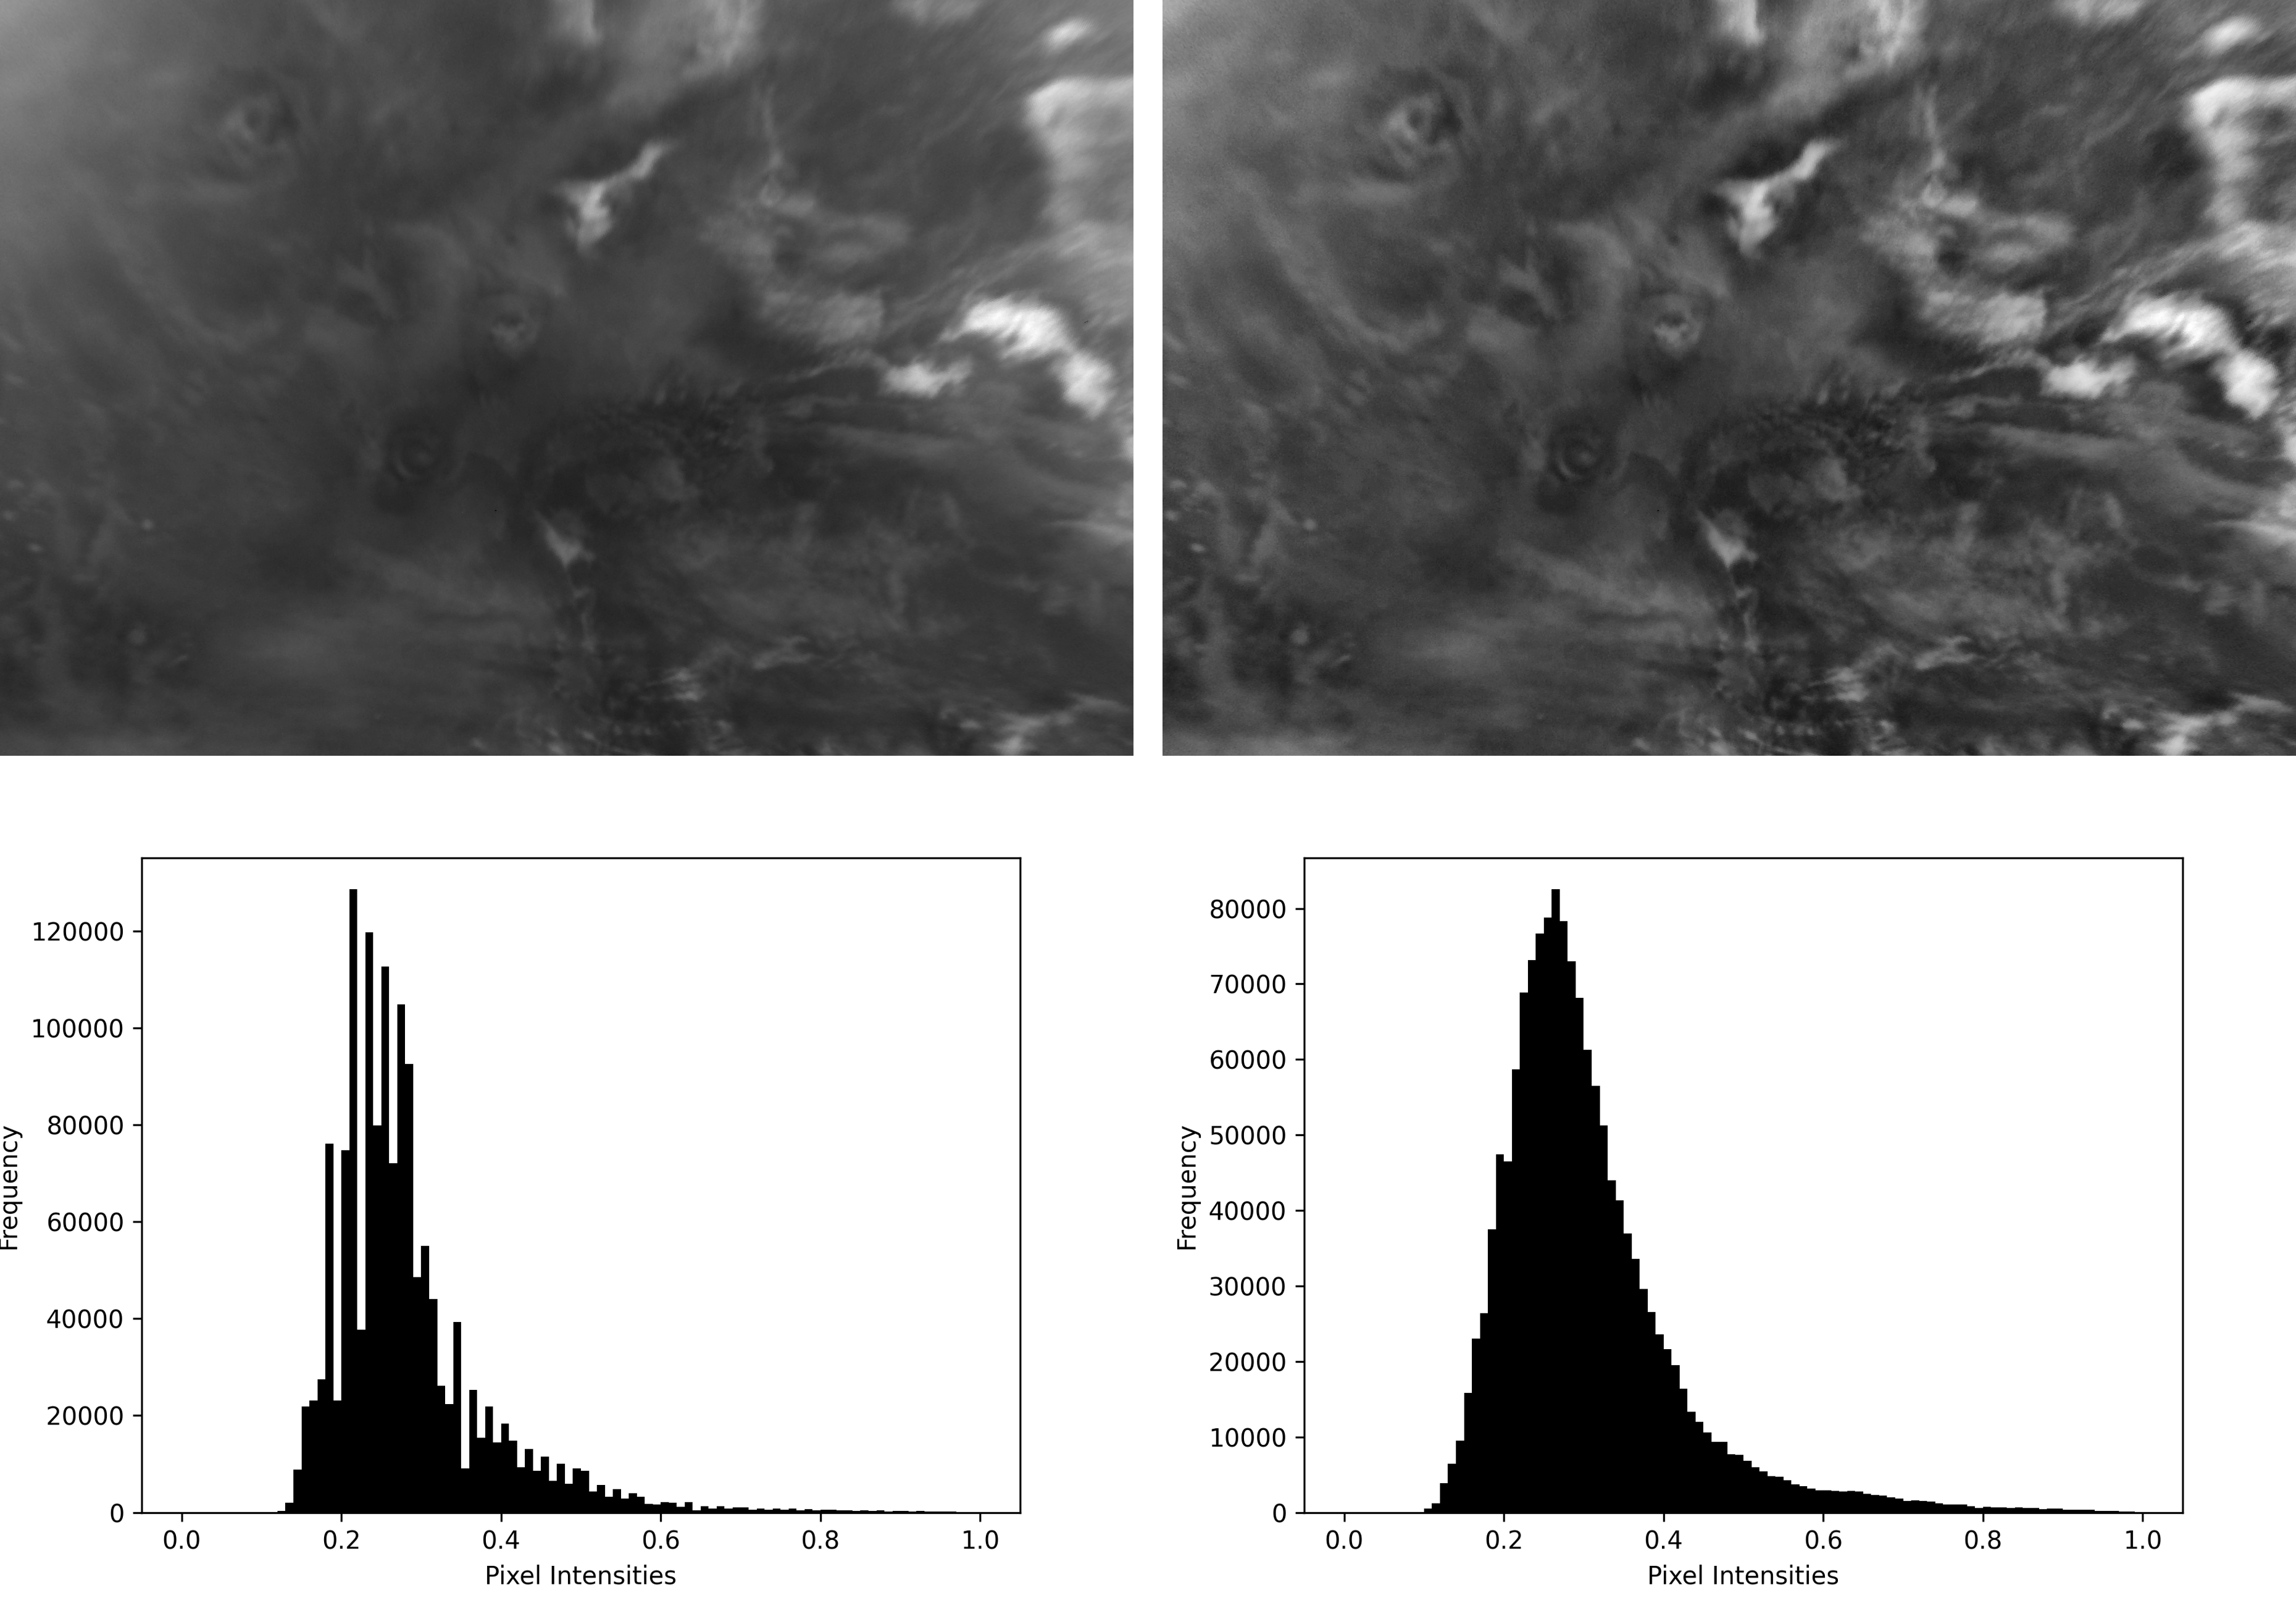
\includegraphics[width=1\textwidth]{fig_23.png}
    \caption{Comparison of raw and CLAHE-transformed image (UTC: 24/12/2021, 10:30:07). The original image including the intensity histogram are on the left, while the CLAHE-transformed image and the intensity histogram are on the right.}
\end{figure}
\FloatBarrier
The transformed images show reduced contrast compared to the histogram-equalized images (see Figure 3.4). However, clouds that were obscured in darker regions are more visible. Additionally, the histograms display smoother transitions.

\subsection{Sigmoid Transformation}

While the previous two methods involved linear transformations of the pixel data, the sigmoid transformation is a non-linear approach. Applying the sigmoid function to the pixel values can enhance details in darker regions while preserving the natural appearance of the image. The sigmoid transformation is given as follows\cite{Braun2000}: 

\begin{equation}
x_{\text{transformed}} = \frac{1}{1 + e^{-\alpha (x - \beta)}}
\end{equation}

where \( x_{\text{transformed}}\) is the transformed pixel value, \( x\) is the input value, \( \alpha\) is the cut-off factor which controls the steepness, and \( \beta\) is the gain factor that controls the midpoint of the curve. The effect of cut-off and gain factors is illustrated in Figure 3.5. 
\FloatBarrier
\begin{figure}[h!] 
    \centering
    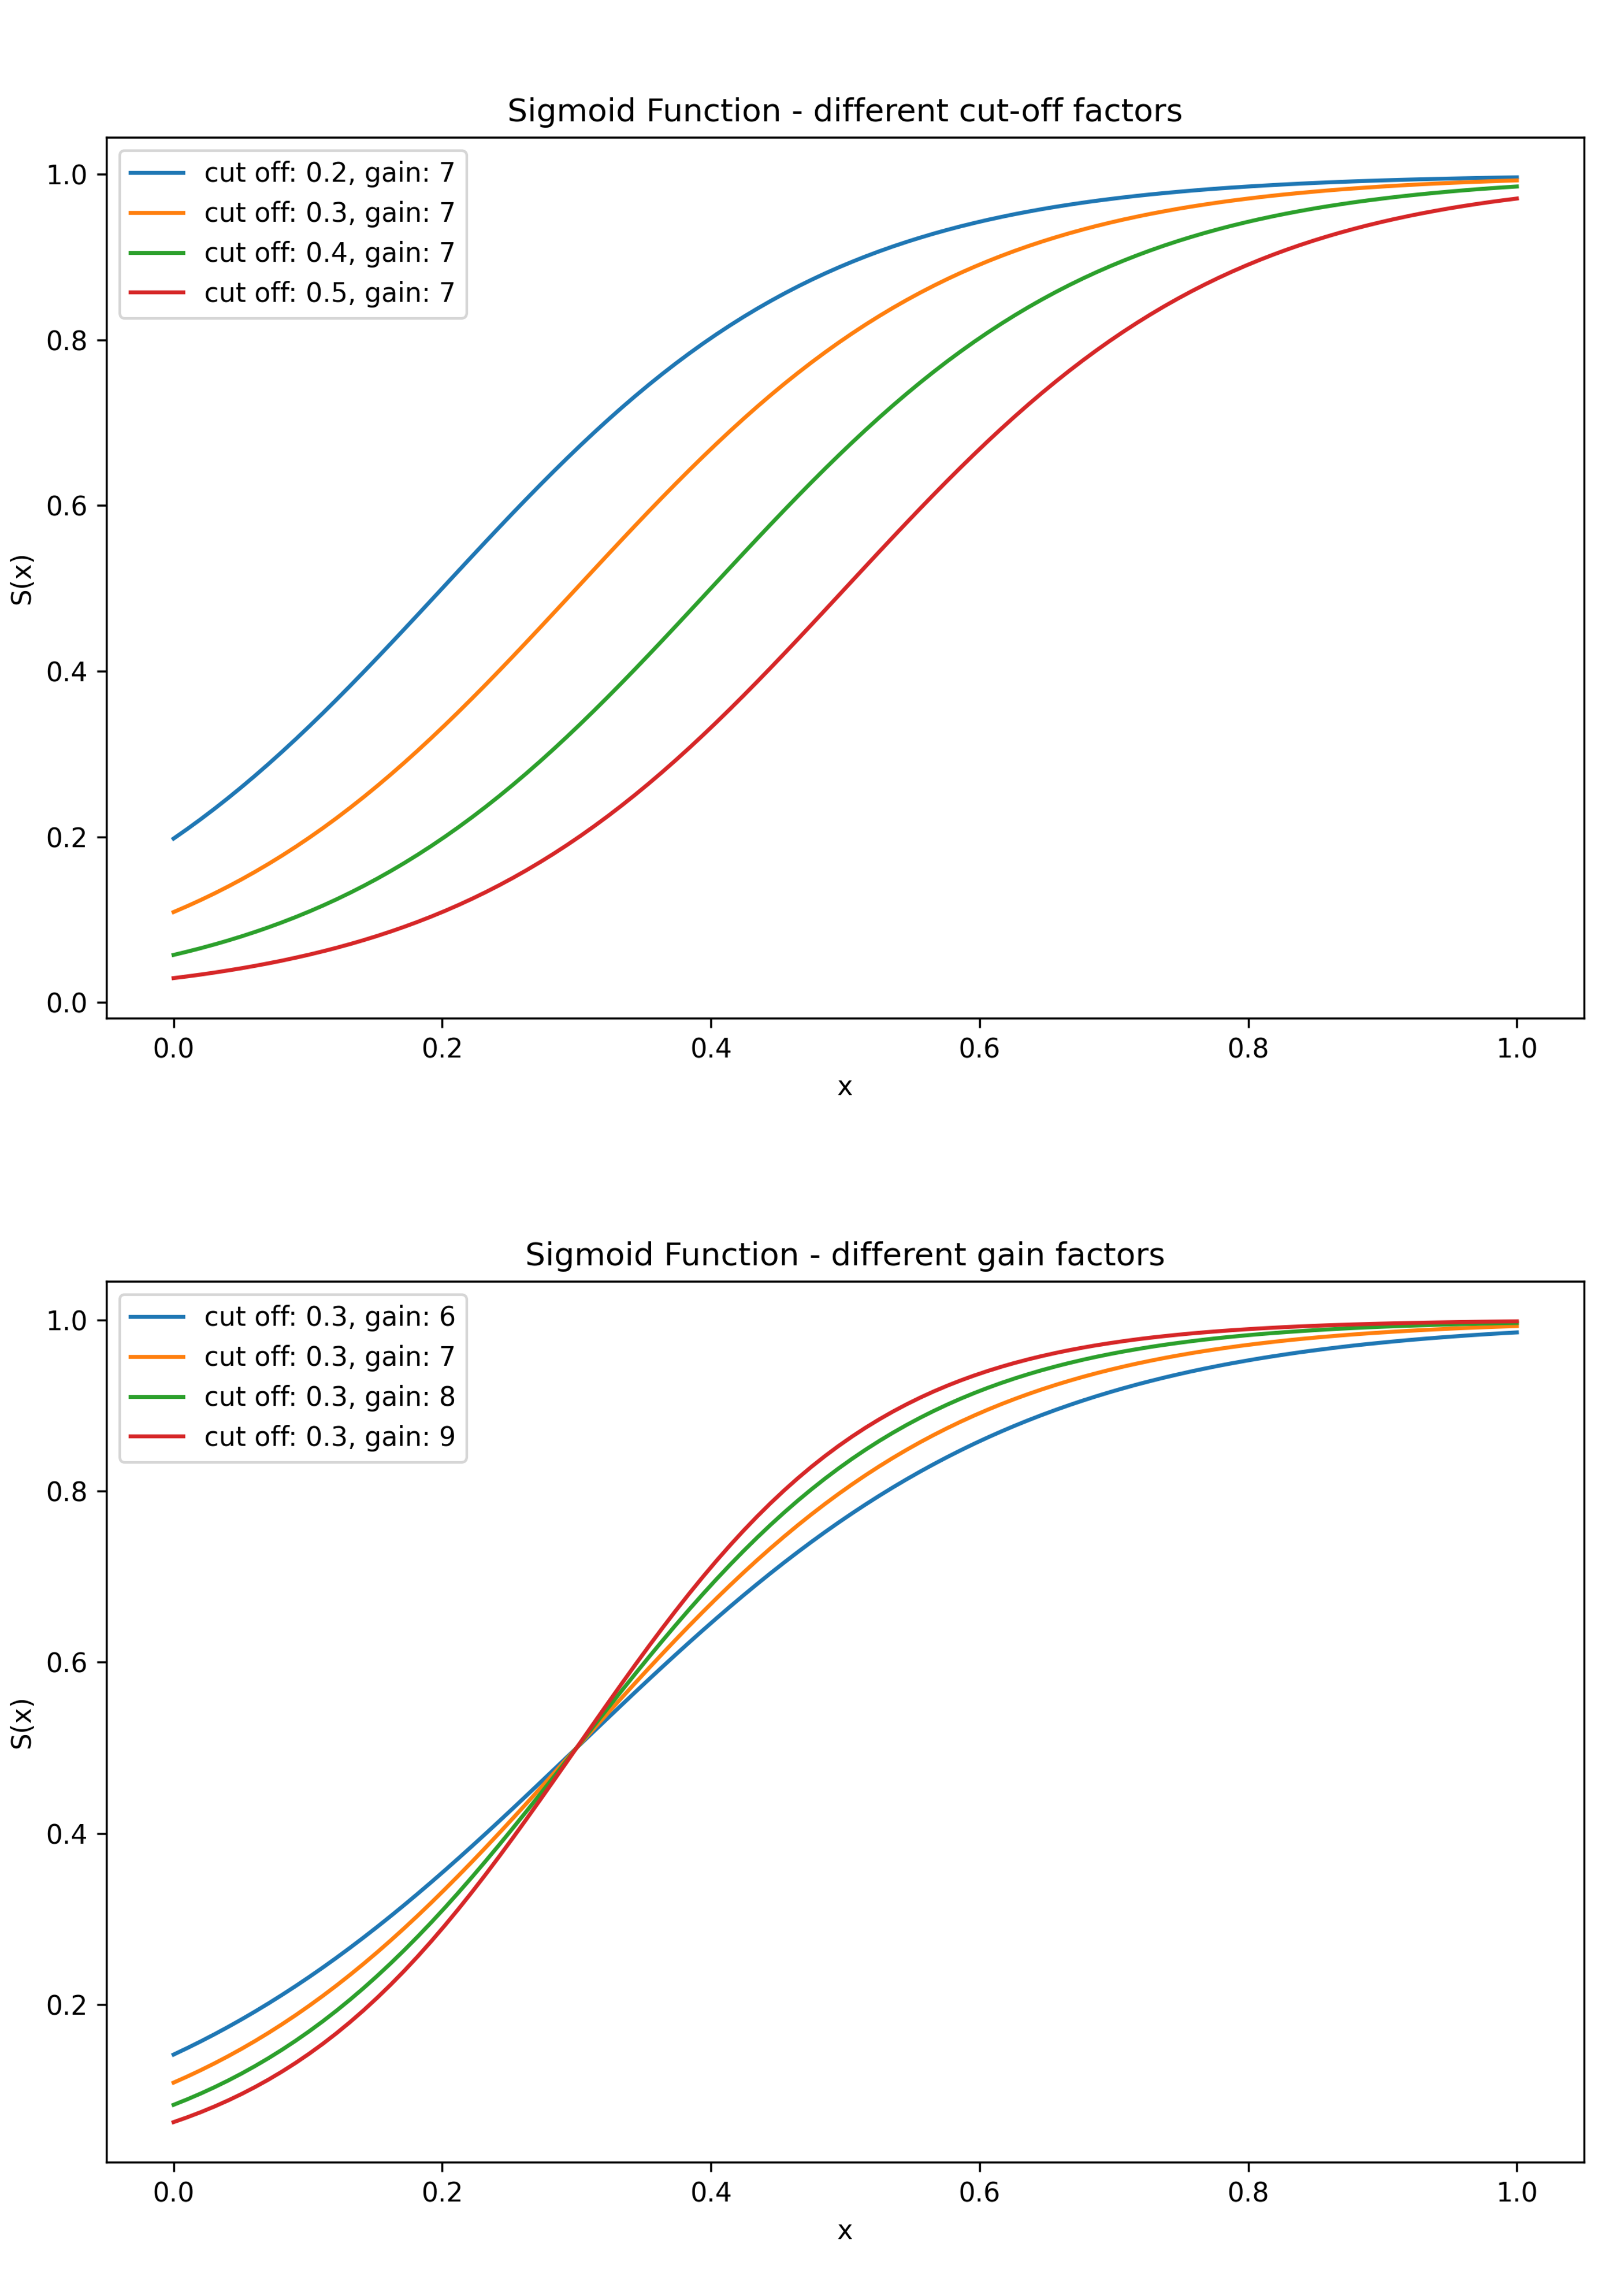
\includegraphics[width=0.8\textwidth]{fig_24.png}
    \caption{Visualisation of the sigmoid function. The plot at the top displays the function with different cut-off factors and the plot at the bottom displays the effect of changing the gain factor.}
\end{figure}
\FloatBarrier
For the given image sequences, the cut-off factor ranged between 0.3 and 0.4 and the gain factor varied between 6 and 8.
\FloatBarrier
\begin{figure}[h!] 
    \centering
    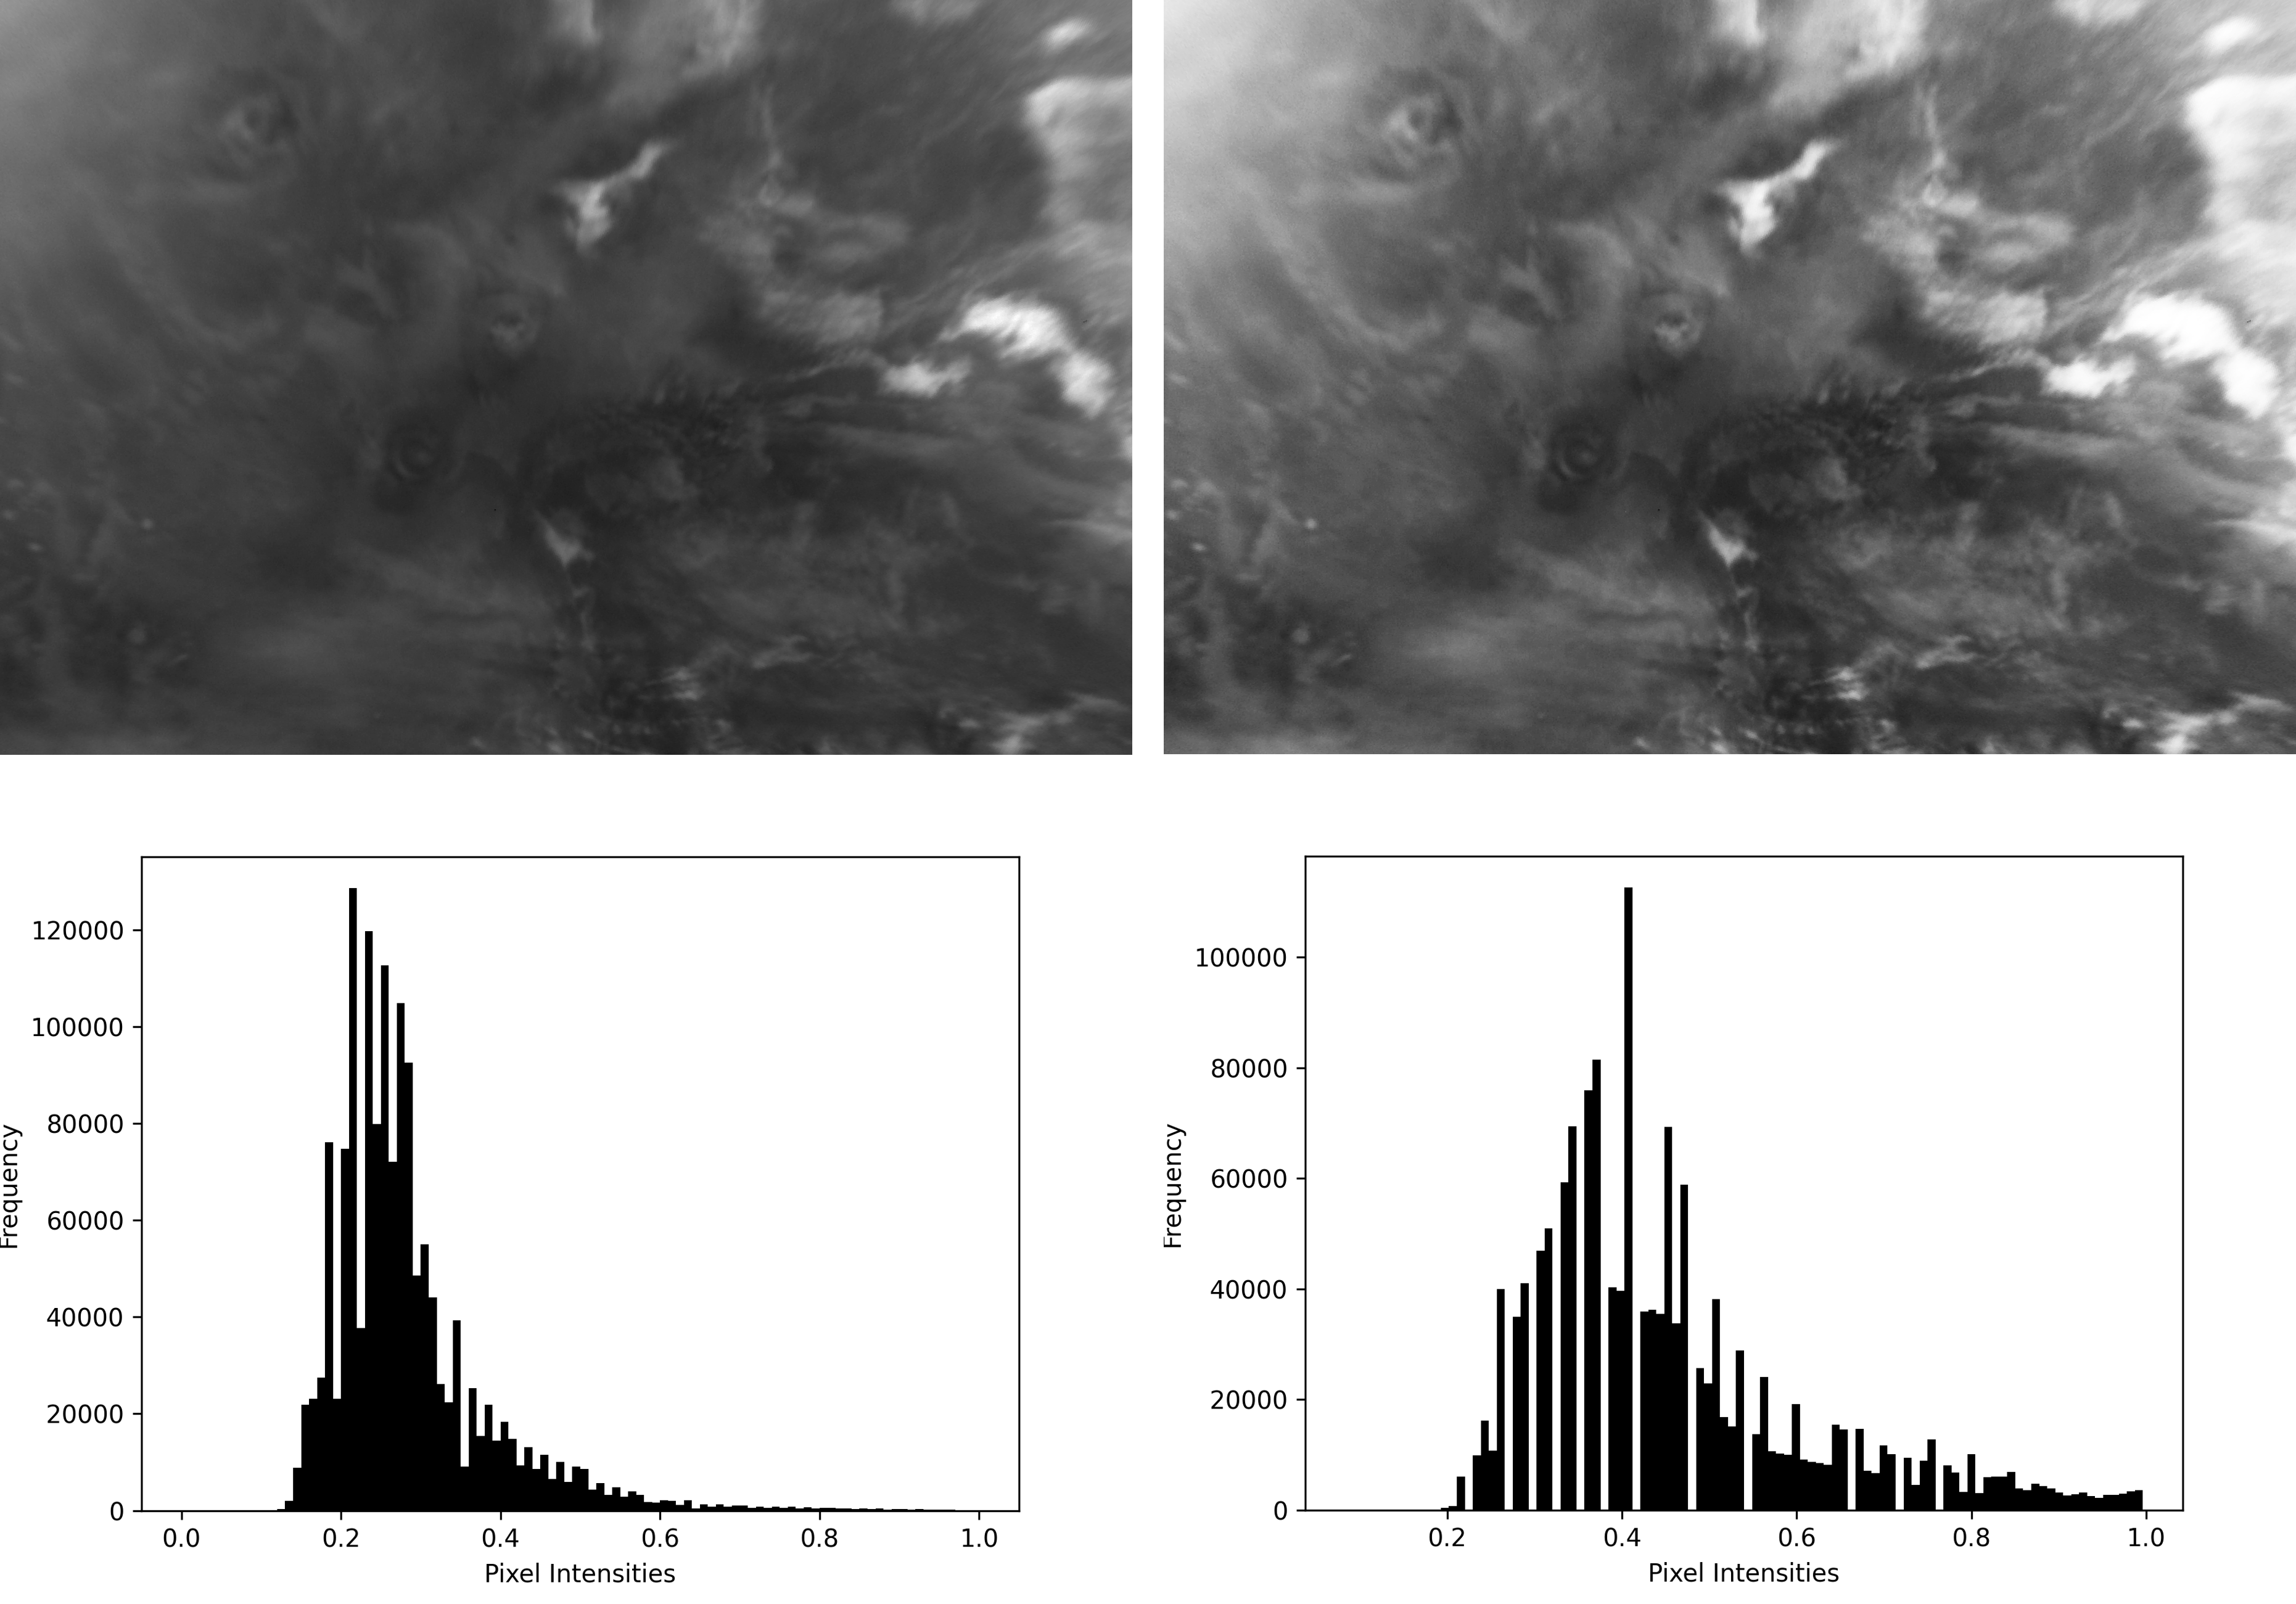
\includegraphics[width=1\textwidth]{fig_25.png}
    \caption{Comparison of raw and sigmoid-transformed image (UTC: 24/12/2021, 10:30:07) with a cut-off factor of 0.3 and a gain factor of 8. The original image including the intensity histogram are on the left, while the sigmoid-transformed image and the intensity histogram are on the right. }
\end{figure}
\FloatBarrier
The resulting images (see Figure 3.6) are brighter, but darker areas haven't been overemphasized. The clouds are more visible, and the histogram retains its shape. However, the pixel intensities are stretched and more evenly distributed.

\section{Cloud Tracking}

To track cloud movements, Correlation Image Velocimetry (CIV) was employed. CIV, a technique based on cross-correlation, was executed using UVMAT — a Matlab-based interface\cite{SoftUVMAT}. After conducting the CIV-analysis, the results were converted into velocity vectors, measured in meters per second. 

\subsection{Correlation Image Velocimetry}

CIV which is a type of Particle Image Velocimetry (PIV), is a motion tracking method. Initially used in fluid mechanics, it has also shown significant utility in tracking clouds in satellite imagery. CIV involves dividing the image into smaller segments, called interrogation windows (as illustrated in Figure 3.7). For each window, velocity vectors are computed by applying cross-correlation to pairs of images\cite{Scharnowski2020} (as shown in Figure 3.8).
\FloatBarrier
\begin{figure}[h!] 
    \centering
    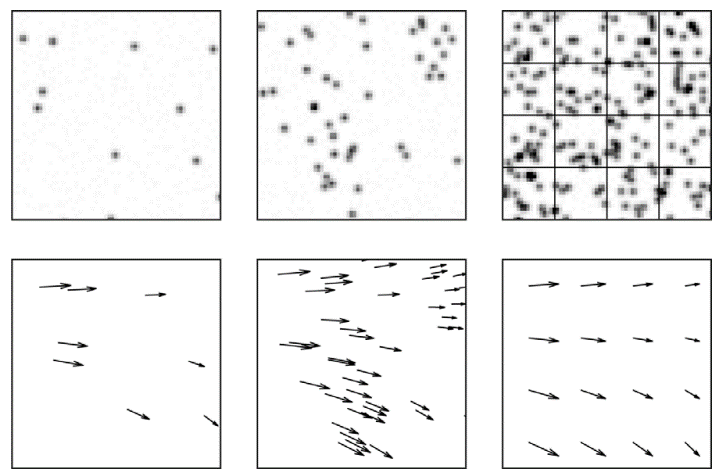
\includegraphics[width=0.7\textwidth]{fig_26.png}
    \caption{Concept visualisation of tracking individual particle images at low (left) and medium (center) density and correlating interrogation windows (right)\cite{Scharnowski2020}. While the images at the top show the particle image distribution, the bottom images display the resulting displacement fields.}
\end{figure}
\FloatBarrier
\begin{figure}[h!] 
    \centering
    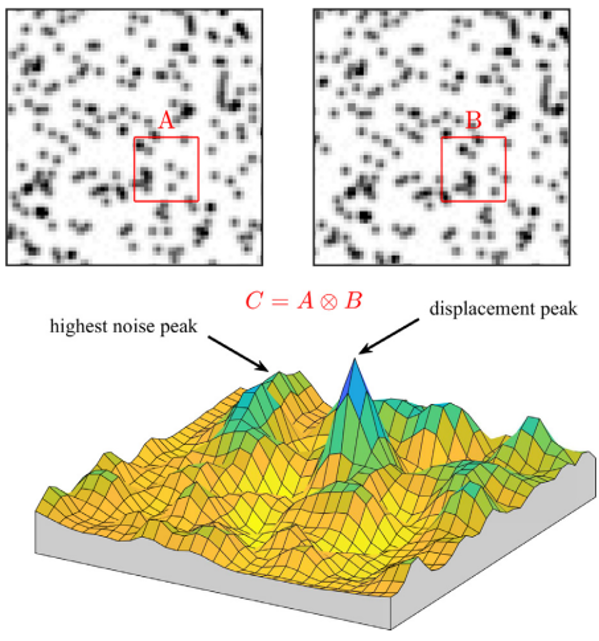
\includegraphics[width=0.7\textwidth]{fig_27.png}
    \caption{Illustration of the cross-correlation process: This example shows a pair of PIV images, capturing the particle distribution at two different times\cite{Scharnowski2020}. The red boxes, each measuring 16 x 16 pixels, highlight the interrogation windows A and B. The bottom image displays the resulting cross-correlation function, where a distinct peak indicates the displacement of the particle images.}
\end{figure}
\FloatBarrier
Using the UVMAT-interface (see Figure 3.9), the images were processed through a six-step process: CIV1, FIX1, PATCH1, CIV2, FIX2, and PATCH2\cite{SoftUVMAT}. 

In the CIV1 stage, initial CIV is performed based on the specified interrogation window and shift box size, where the latter defines the area within which CIV is allowed to detect movements, while the grid size determines the number of vectors displayed. The FIX1 stage corrects errors and filters vectors above a pre-defined correlation co-efficient. PATCH1 applies a smoothness filter using interpolation and determines the maximum vector size. 
CIV2, FIX2 and PATCH2 repeat the process using vectors obtained from CIV1, additionally allowing for refined parameter adjustments and accounting for rotation and deformation.
\FloatBarrier
\begin{figure}[h!] 
    \centering
    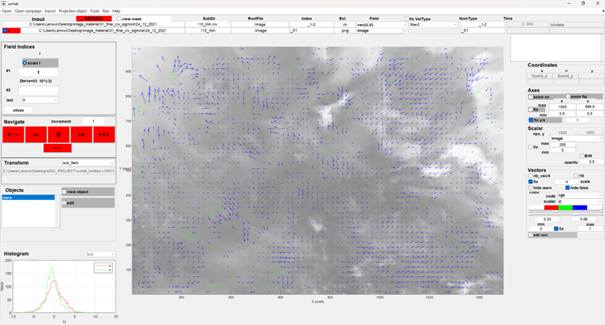
\includegraphics[width=1\textwidth]{fig_28.png}
    \caption{Screenshot of the UVMAT interface used for performing CIV\cite{SoftUVMAT}.}
\end{figure}
\FloatBarrier
The parameters (see Figure 3.10), were set based on visual observations and cloud features sizes. 
The interrogation window size was chosen to be sufficiently large to maximize detection probability while avoiding excessive size that could lead to mismatches. Similarly, the shift box was sized to match small cloud features to ensure efficient movement detection. Ideally, the correlation box should be kept as small as possible; however, if too small, there are insufficient pixels for accurate matching, leading to reduced correlation and an increase in false vectors.

The grid size should also match the size of the correlation area: a smaller grid leads to oversampling, whereas a larger grid provides too few vectors. In this instance, a slightly smaller grid size was defined to enhance result visualization by increasing vector density.

Additionally, the choice of time interval is important. A longer time interval can yield more accurate velocity vector measurements. However, if the interval is excessively long, cloud deformation over time renders the movements undetectable.
\FloatBarrier
\begin{figure}[h!] 
    \centering
    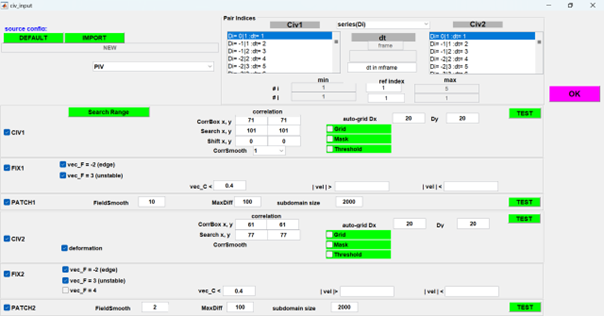
\includegraphics[width=1\textwidth]{fig_29.png}
    \caption{Screenshot of the CIV parameters used in this thesis.}
\end{figure}
\FloatBarrier
\subsection{Velocity Field Extraction}

To extract velocity fields, the results from CIV were imported into Python. The data was converted from pixel coordinates (x and y) to longitude and latitude, and from the zonal (u) and meridional (v) components, measured in pixels per time unit, to meters per second. The magnitude was calculated by determining the Euclidean distance between the u and v components, divided by the time interval. 

The transformation of CIV \( x\) and \( y\) coordinates into longitude and latitude in degrees was performed using the following formulas\cite{AlBlooki2023}: 

\begin{equation}
lon = \lambda_w + (\lambda_e - \lambda_w) \cdot \frac{x_{\text{civ}}}{n_x}
\end{equation}

\begin{equation}
lat = \phi_n + (\phi_s - \phi_n) \cdot \frac{y_{\text{civ}}}{n_y}
\end{equation}

\( \lambda_e\) and \( \lambda_w\) denote the eastern and western limits of the longitude grid, while \( \phi_n\) and \( \phi_s\) represent the northern and southern limits of the latitude grid. \( n_x\) indicates the total number of pixels along the x-axis, and \( n_y\) represents the total number of pixels along the y-axis.

The conversion of pixel per time separation to \( m s^-1\) was done as follows:
\begin{equation}
u = \frac{u_{\text{civ}}}{\triangle t} \cdot \frac{\lambda_e - \lambda_w}{\triangle x} \cdot \frac{\pi}{180} \cdot r \cdot \cos(\phi)
\end{equation}

\begin{equation}
v = \frac{v_{\text{civ}}}{\triangle t} \cdot \frac{\phi_n - \phi_s}{\triangle y} \cdot \frac{\pi}{180} \cdot r
\end{equation}

Where \( \triangle t\) is 600 or 1800 depending on the image sequence, \( \triangle x\) = \( \triangle y\) is 0.0625°/pixel,  \( \phi_n\) and \( \phi_s\) are the planetocentric latitudes and \( r\) is the radius of Mars (3389500 meters). \( \cos(\phi)\) is the cosine of the latitude factor, included to account for the variation in latitudinal distance. Figure 3.11 illustrates the geometric and trigonometric relationships that form the basis for the properties of latitude and longitude.
\FloatBarrier
\begin{figure}[h!] 
    \centering
    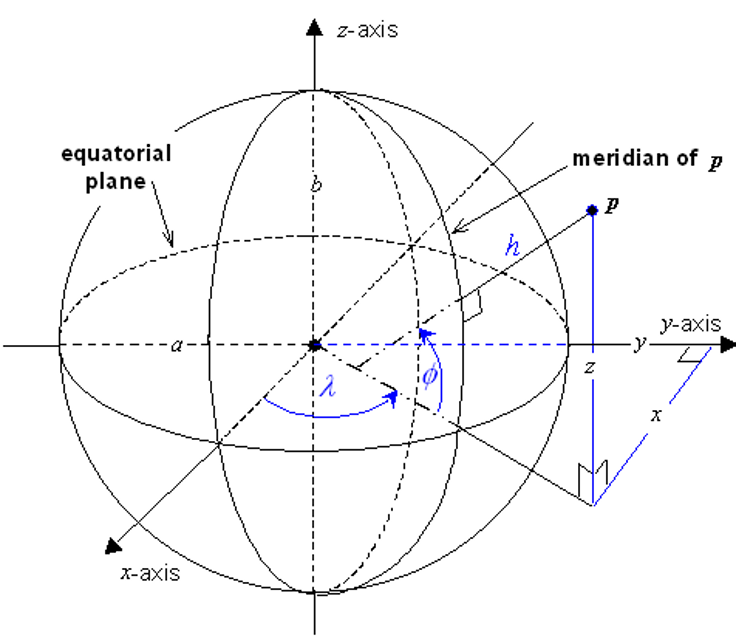
\includegraphics[width=0.8\textwidth]{fig_30.png}
    \caption{Illustration of the geodetic coordinate system geometric and trigonometric relationships\cite{ISO18026}.}
\end{figure}
\FloatBarrier
\chapter{Results\label{chap:results}}

This section covers a comparison of the image processing techniques, a CIV performance analysis for the differently processed images and the analysis of the resulting wind fields.

\section{Comparison of Image Processing Techniques}
\FloatBarrier
\begin{figure}[h!] 
    \centering
    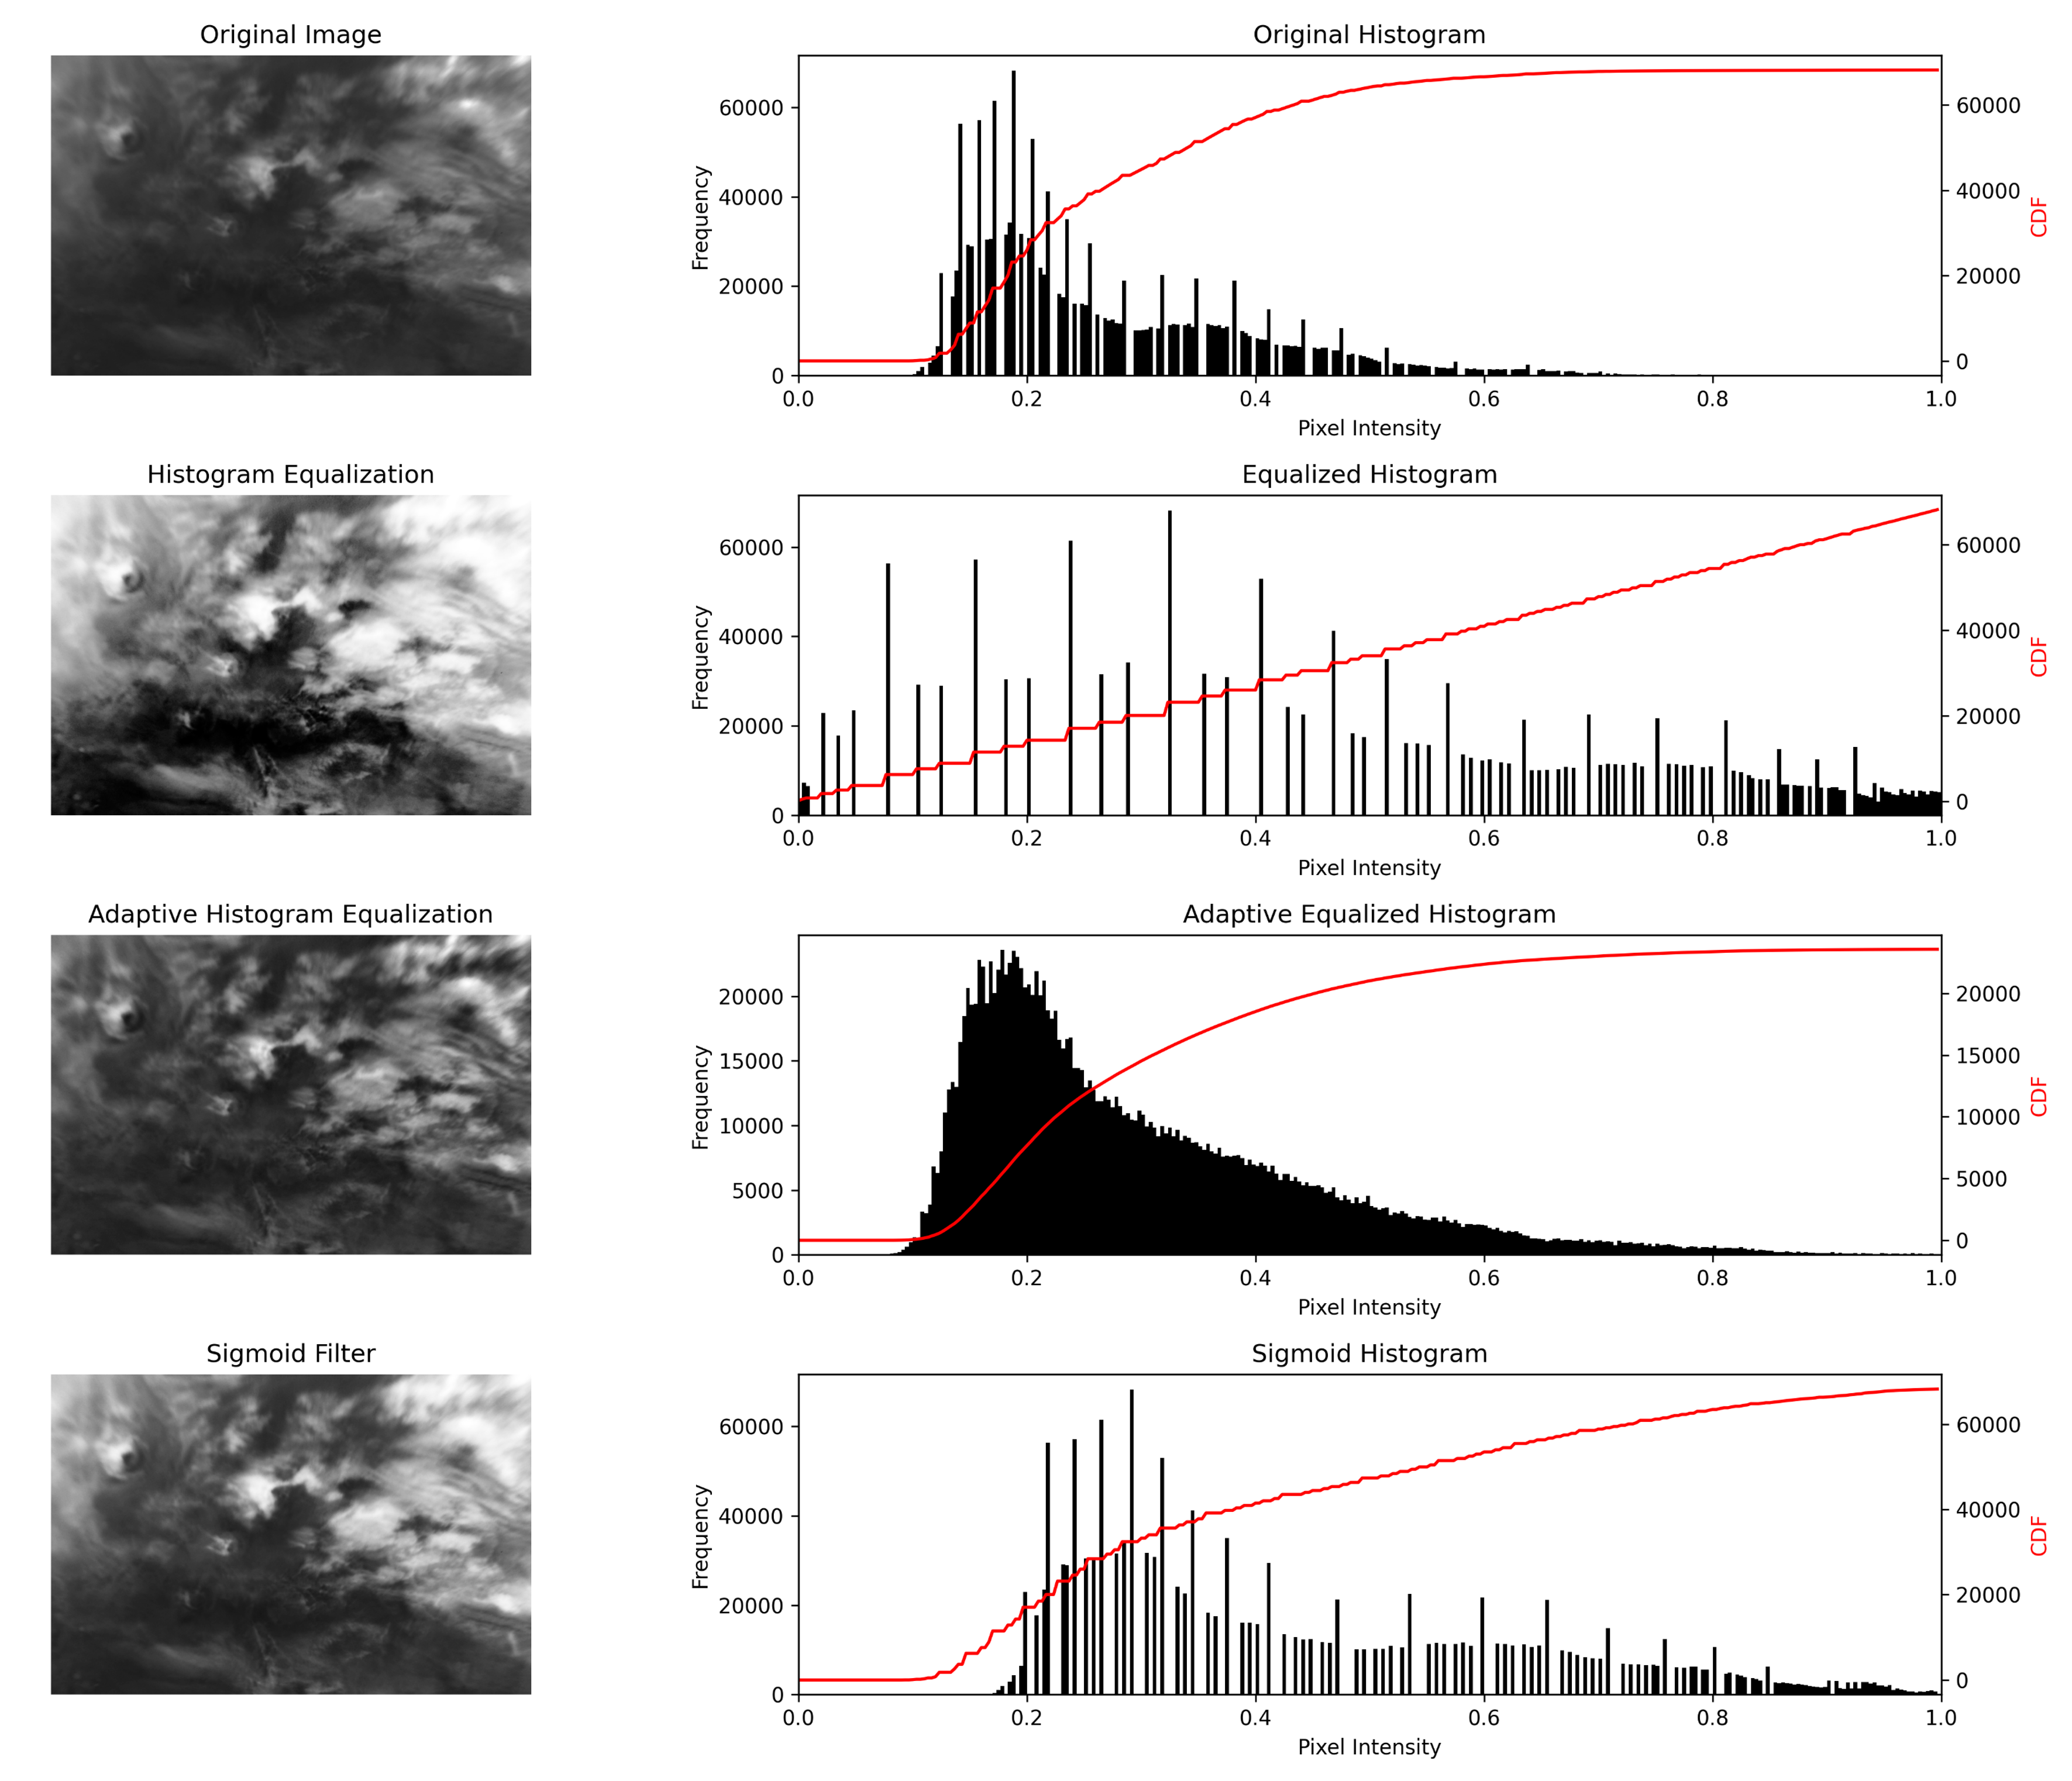
\includegraphics[width=0.9\textwidth]{fig_31.png}
    \caption{overview of differently processed image versions from UTC: 22/11/2021 14:16:52.}
\end{figure}
\FloatBarrier
When comparing the visual results of the image enhancement methods (see Figure 4.1), the sigmoid filter stands out as particularly effective. It enhances the images by brightening them to reveal clouds that were visually hidden in darker pixels, without over-intensifying the lighter areas. In contrast, HE tends to overemphasize bright pixels, leading to high contrast that obscures fine details. CLAHE performs somewhat better, however, potentially results in a disproportionate representation of intensity levels in sub-regions.

As evidenced by the histogram and CDF, the sigmoid filter appears to preserve the original data more effectively. The histogram shows maintains its original shape but shifts to the right. Similarly, the CDF remains similar although flattened.

\section{CIV - Performance Comparison}

After performing CIV on the differently processed images, the average correlation coefficient  after removal of warning and error flags and the percentage of warning and error flags were analysed.
\FloatBarrier
\begin{figure}[h!] 
    \centering
    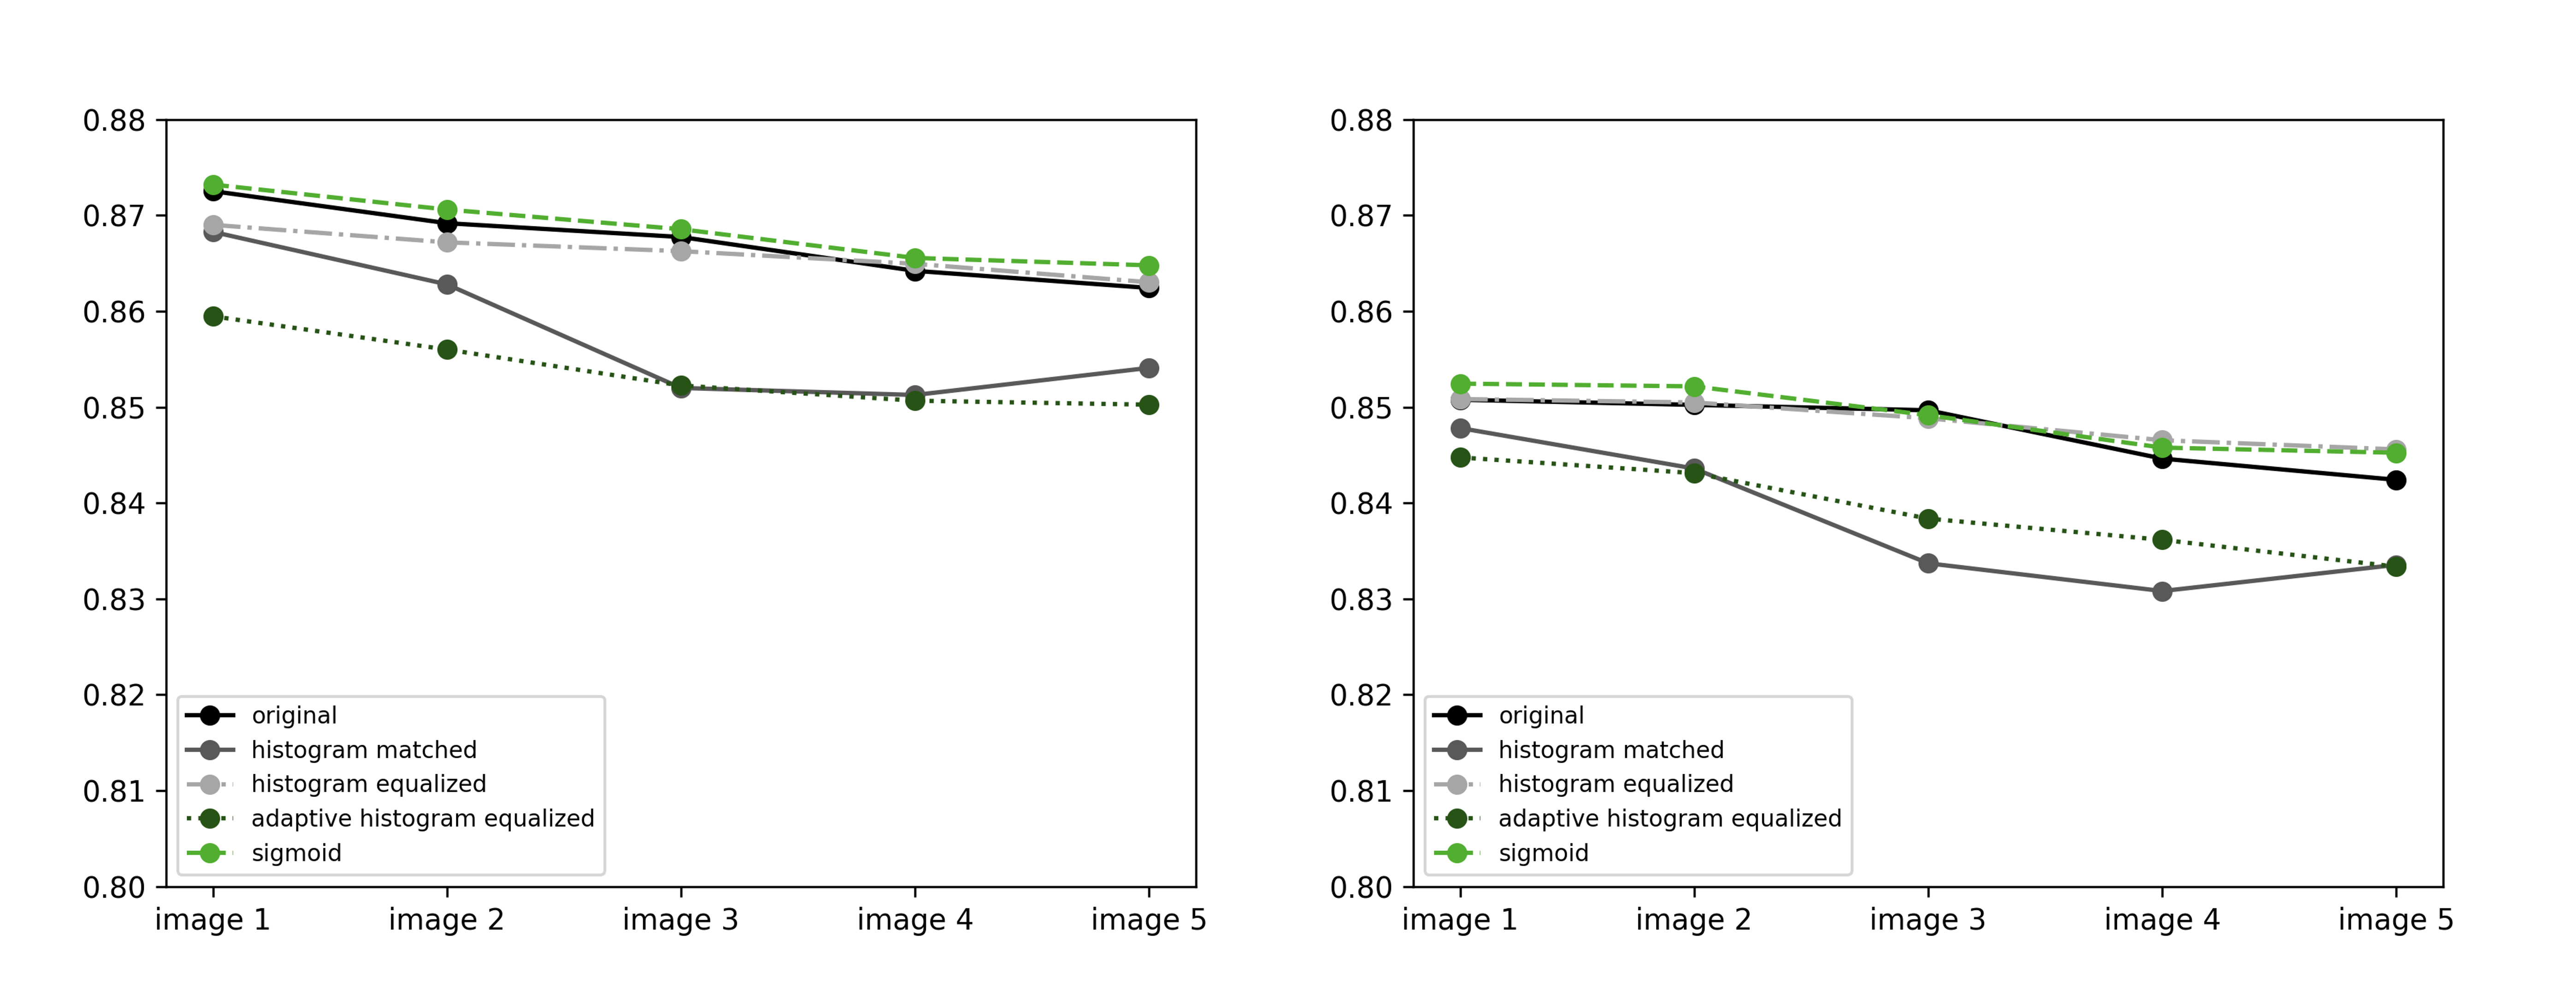
\includegraphics[width=1\textwidth]{fig_32.png}
    \caption{Plot of the average correlation co-efficient of vector fields identified during CIV1 (left) and CIV2 (right) for each image transition. Vectors with error flags were removed before the calculation. The data source of this visualisation are 6 images from 24/12/2021 ranging over the time span 10:30:07 - 11:20:06 with a time separation of 10 minutes.}
\end{figure}
\FloatBarrier
The average correlation co-efficient determined during the CIV process across each image sequence is generally high at around 0.8, however, different image processing techniques lead to changes in the performance (as displayed in figure 4.2). 
Analysing the CIV results of each image sequence, the original, sigmoid transformed and HE images have a higher average correlation co-efficient than the histogram matched and CLAHE images.
\FloatBarrier
\begin{figure}[h!] 
    \centering
    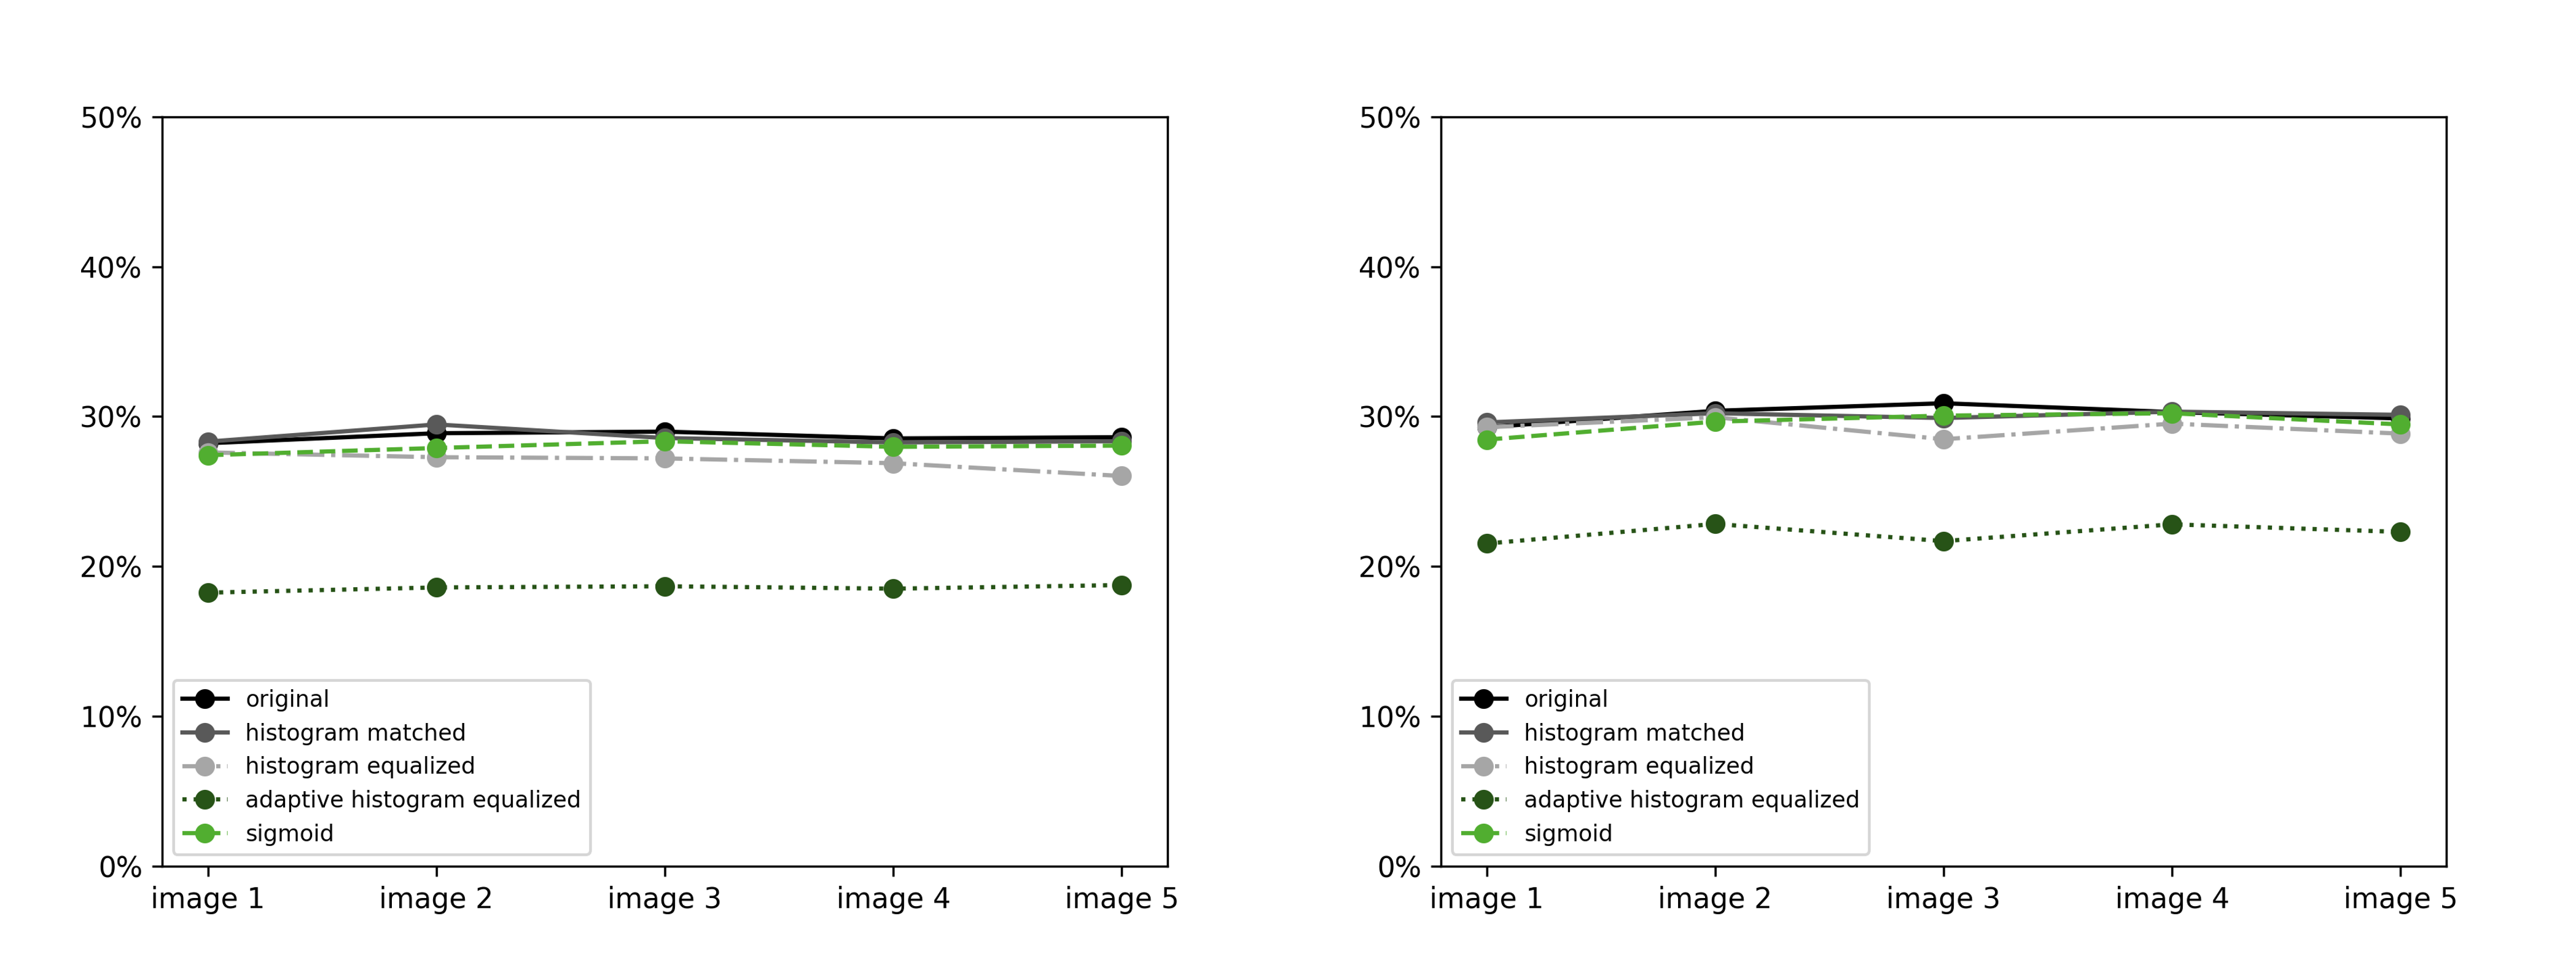
\includegraphics[width=1\textwidth]{fig_33.png}
    \caption{Plot of the amount FF errors displayed in percentages of the total number of vectors identified during CIV1 (left) and CIV2 (right) for each image transition. The data source of this visualisation are 6 images from 24/12/2021 ranging over the time span 10:30:07 - 11:20:06 with a time separation of 10 minutes.}
\end{figure}
\FloatBarrier
The percentages of FF error flags (see Figure 4.3), which highlight irregularities in the calculation of velocity vectors\cite{TutorialUVMAT}, are relatively consistent across most methods, except for CLAHE. 
The reduced occurrence of false vectors in CLAHE-processed images might be attributed to the suppression of noise and improved visibility of features. The reduced number of error flags in CLAHE-processed sequences may contribute to the lower correlation coefficient, due to the presence of additional velocity vectors, lowering the overall average.
\FloatBarrier
\begin{figure}[h!] 
    \centering
    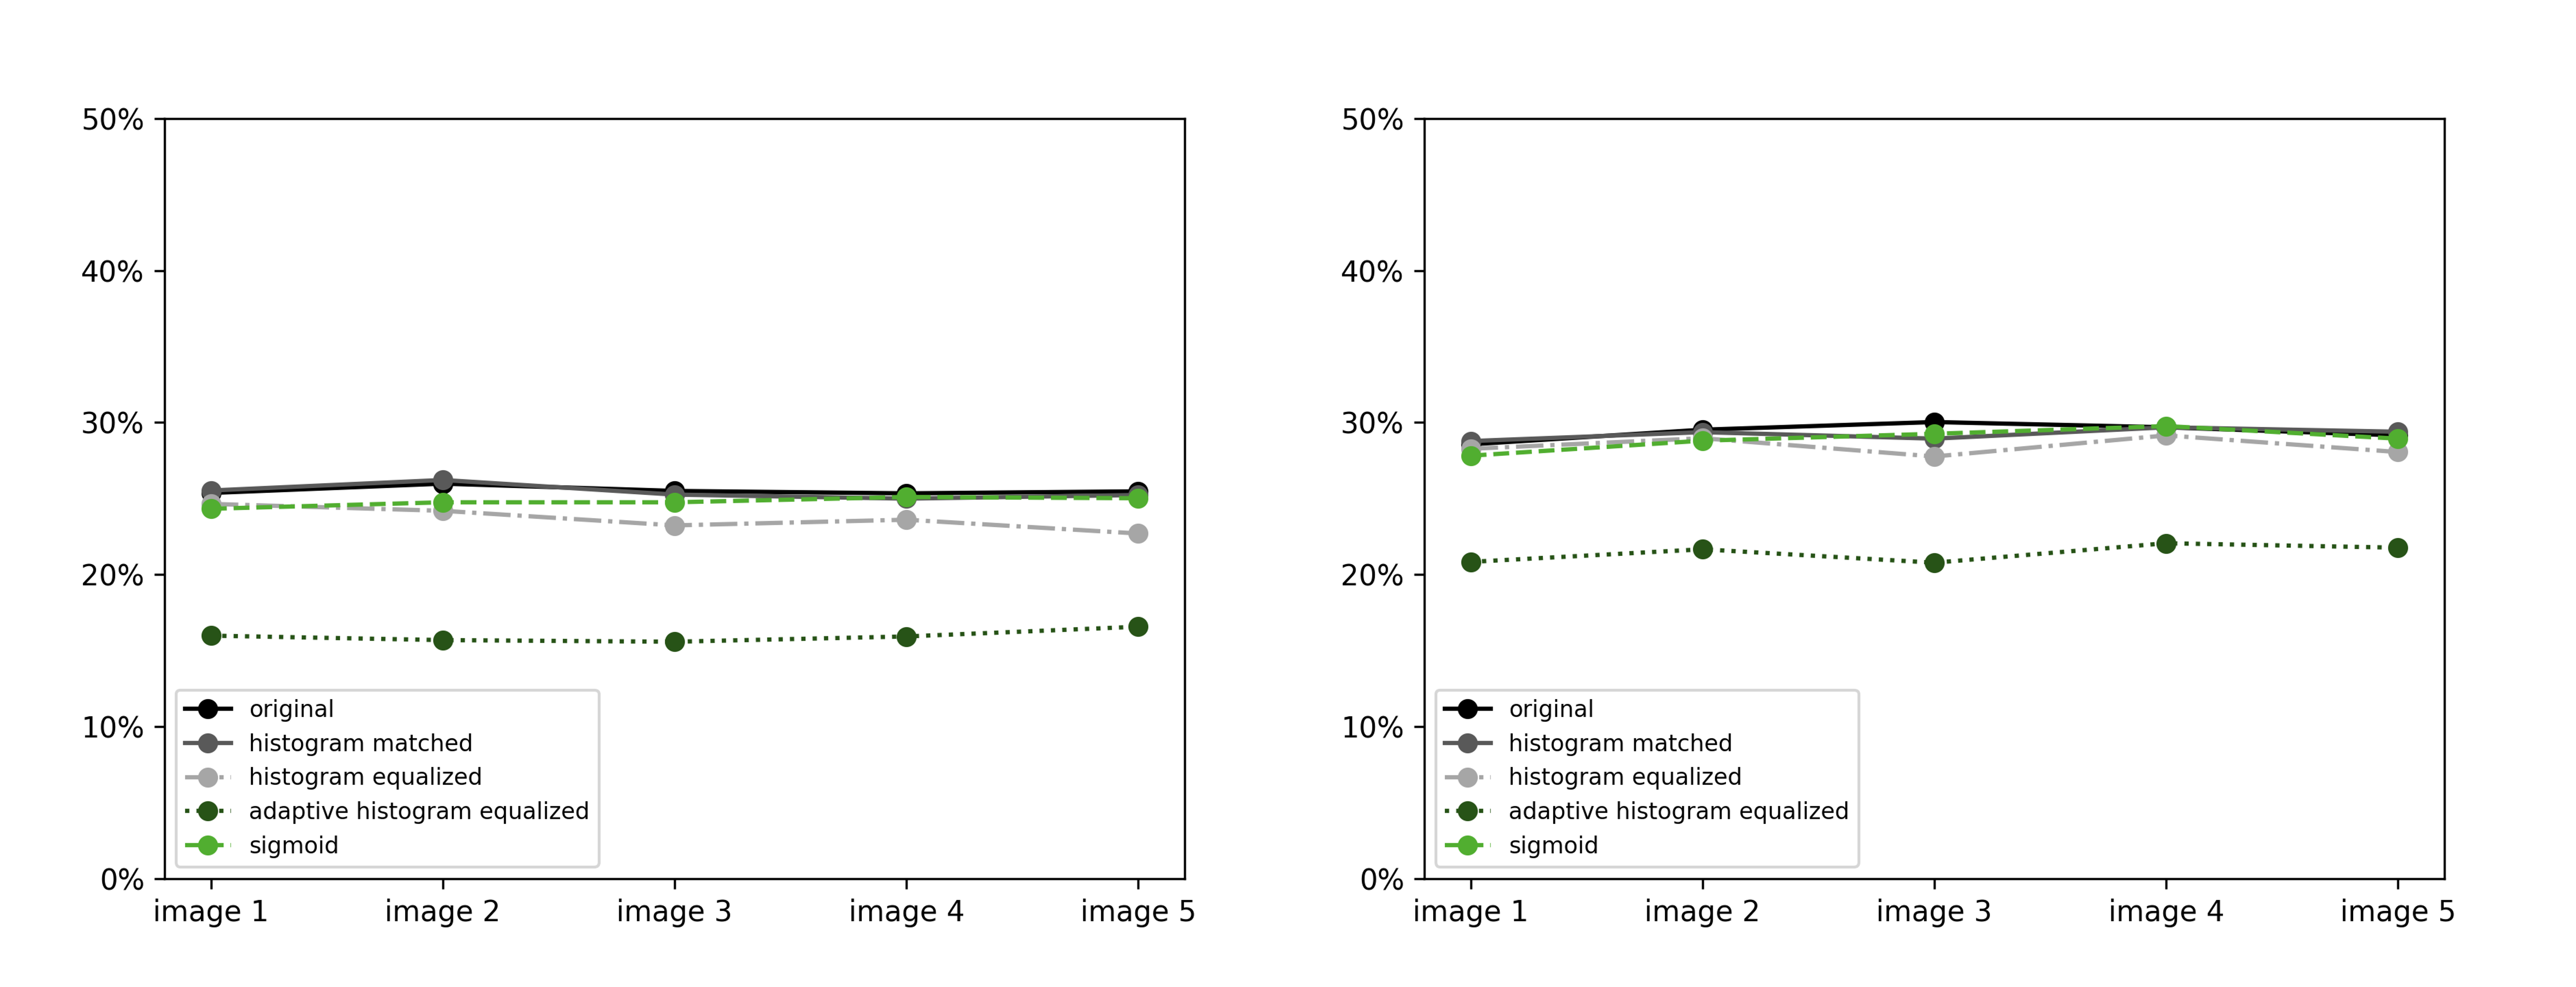
\includegraphics[width=1\textwidth]{fig_34.png}
    \caption{Plot of the amount F warnings displayed in percentages of the total number of vectors identified during CIV1 (left) and CIV2 (right) for each image transition. The data source of this visualisation are 6 images from 24/12/2021 ranging over the time span 10:30:07 - 11:20:06 with a time separation of 10 minutes.}
\end{figure}
\FloatBarrier
F warning flags (as shown in Figure 4.4) usually indicate, that the search domain is too small\cite{TutorialUVMAT}, as they account for vectors where the highest correlation was found at the edge of the search box. The number of warning flags is relatively consistent across all processing methods, with the exception of CLAHE, where the count is lower. Given that the search box size was uniform for all images, this lower number of flags in CLAHE-processed images suggests that correlations are being detected that are missed in images processed with other techniques. While this could indicate improved detection, it may also point to the presence of false vectors resulting from altered pixel intensities that do not reflect the image's natural state.

\section{Velocity Fields}

Building on the earlier comparison, CLAHE image sequences were chosen for the final velocity fields. Despite the lower average correlation coefficient, the use of CLAHE images led to fewer error and warning flags, resulting in a greater number of velocity fields within the image. Upon visual inspection, additional vectors that were absent in other images appeared reasonable and did not seem to result from incorrect detection. The resulting velocity fields for the first transition in each image sequence are shown in Figures 4.5 through 4.10.
\FloatBarrier
\begin{figure}[h!] 
    \centering
    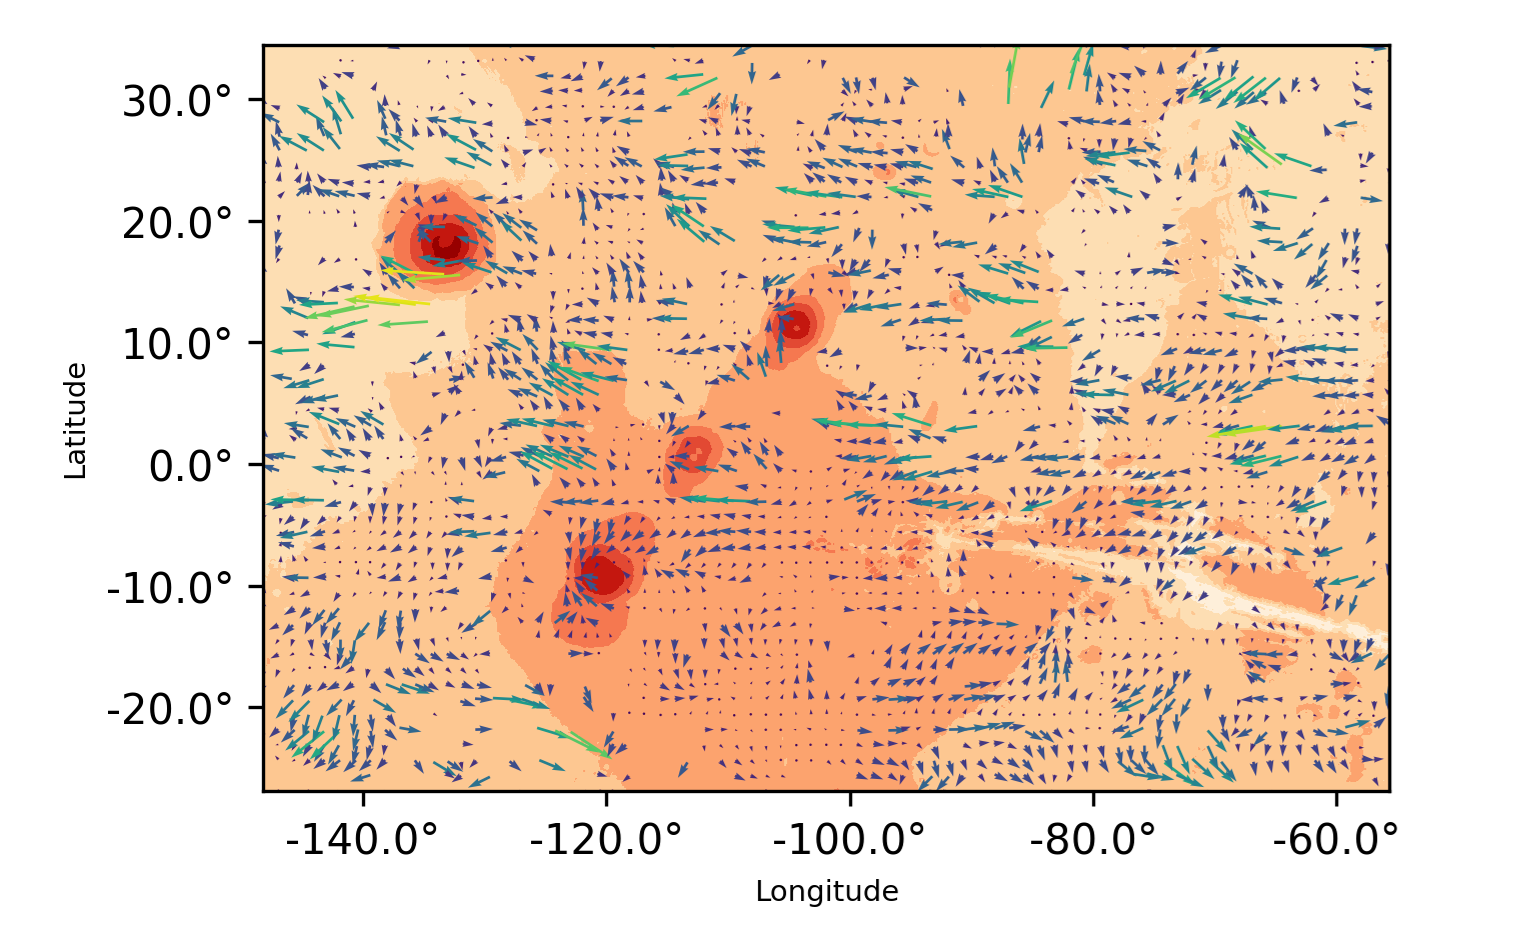
\includegraphics[width=1\textwidth]{fig_35.png}
    \caption{Velocity fields - UTC: 22/11/2021 14:16:52 - 14:26:52}
\end{figure}
\FloatBarrier
\begin{figure}[h!] 
    \centering
    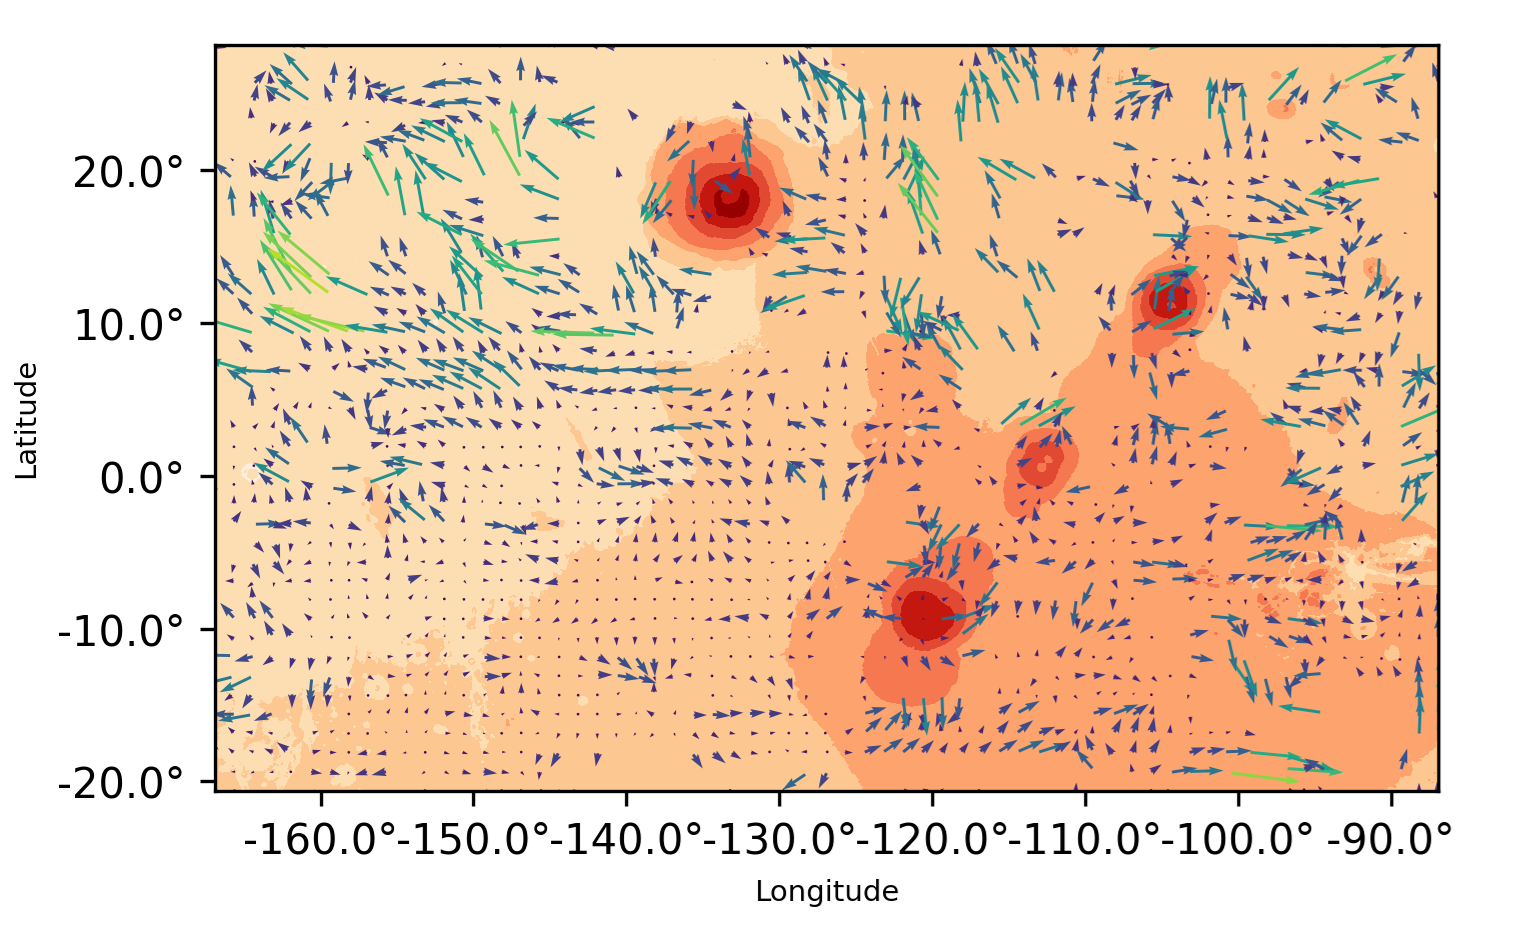
\includegraphics[width=1\textwidth]{fig_36.png}
    \caption{Velocity fields - UTC: 04/12/2021 00:31:53 - 00:41:53}
\end{figure}
\FloatBarrier
\begin{figure}[h!] 
    \centering
    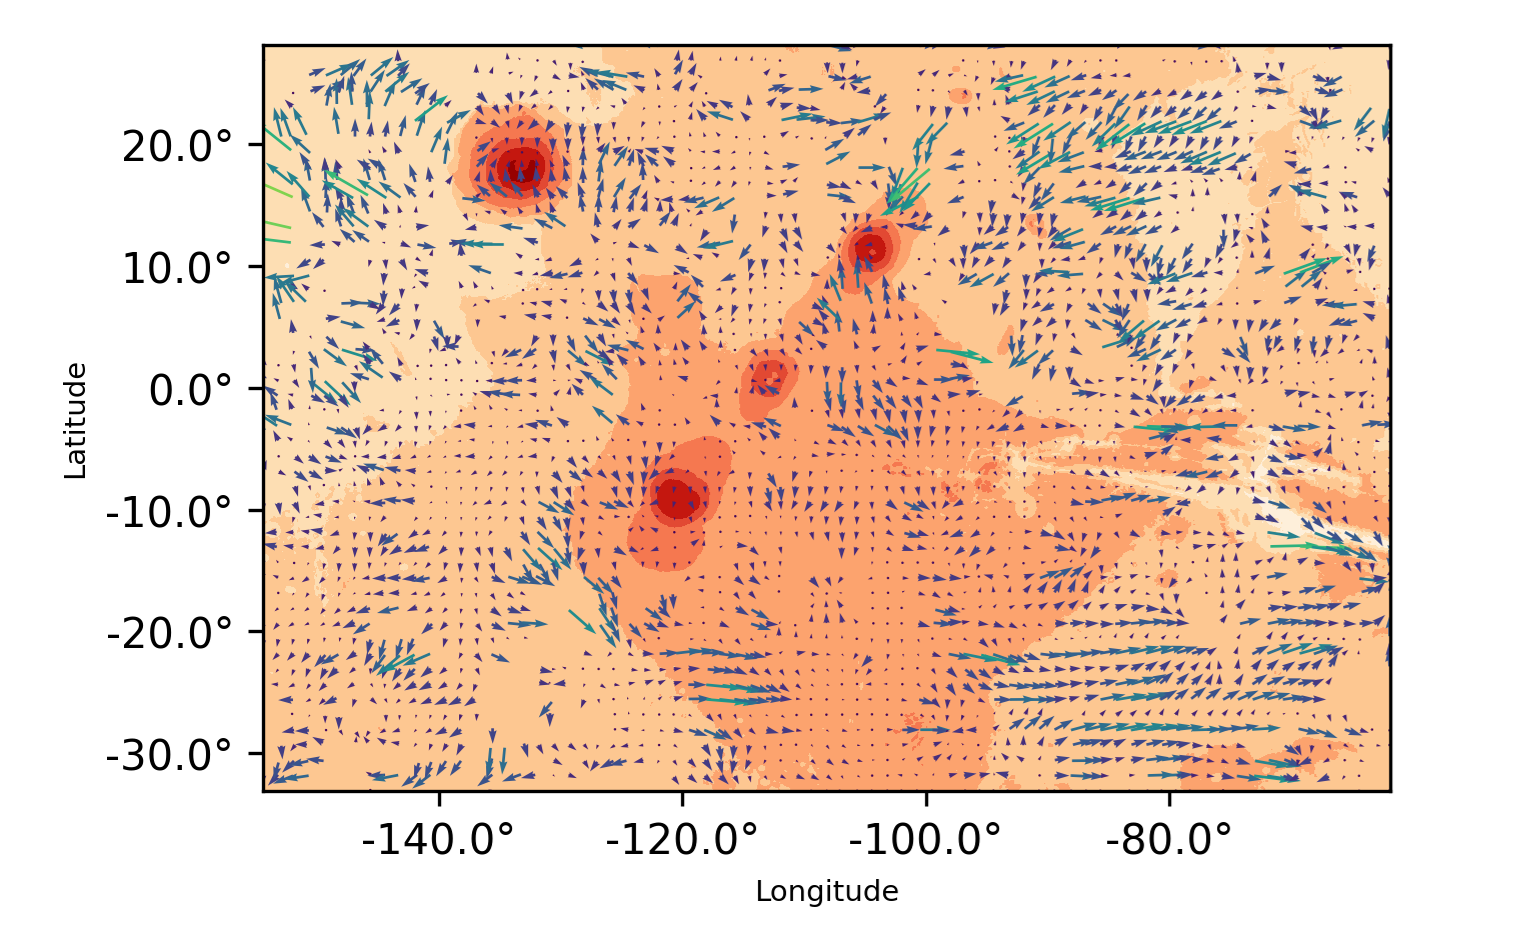
\includegraphics[width=1\textwidth]{fig_37.png}
    \caption{Velocity fields - UTC: 24/12/2021 10:30:07 - 10:40:06}
\end{figure}
\FloatBarrier
\begin{figure}[h!] 
    \centering
    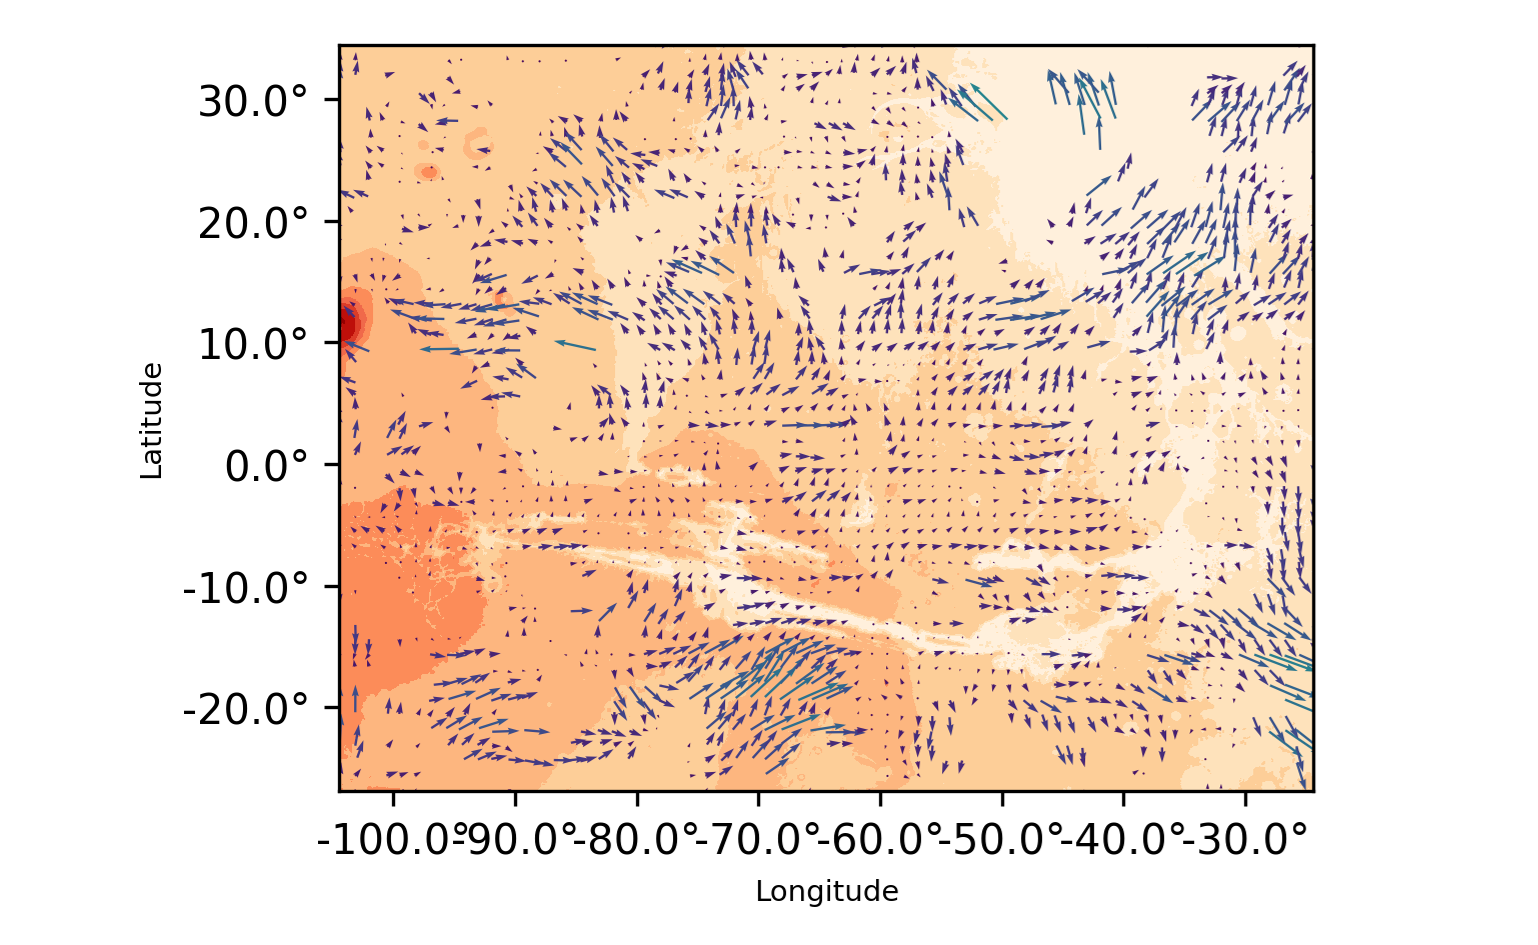
\includegraphics[width=1\textwidth]{fig_38.png}
    \caption{Velocity fields - UTC: 23/10/2023 05:40:13 - 06:10:16}
\end{figure}
\FloatBarrier
\begin{figure}[h!] 
    \centering
    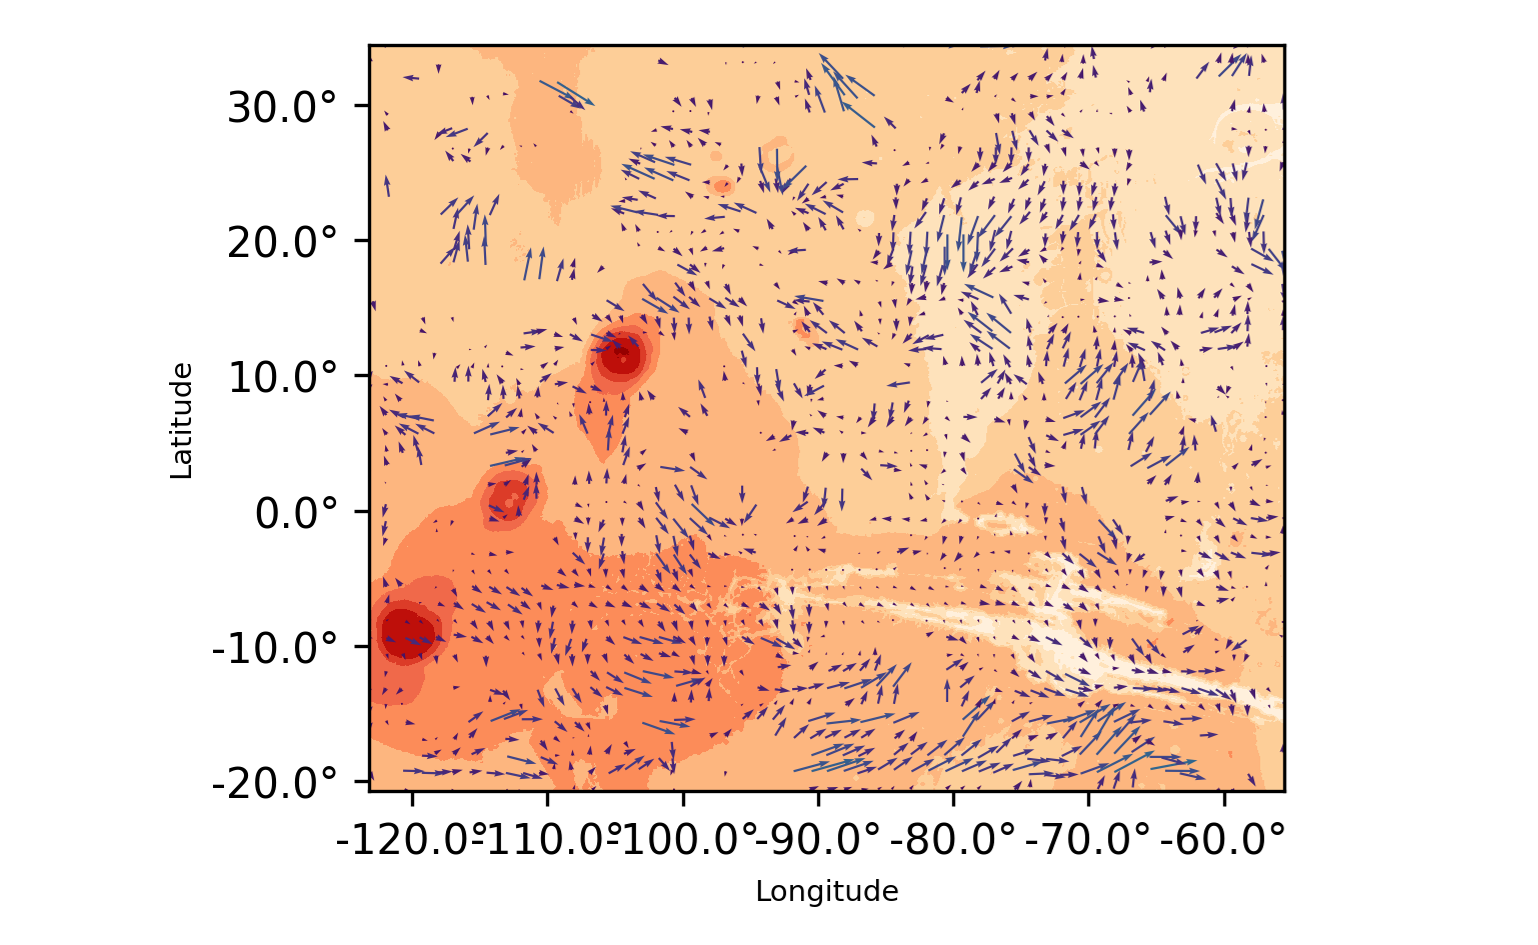
\includegraphics[width=1\textwidth]{fig_39.png}
    \caption{Velocity fields - UTC: 23/10/2023 08:18:33 - 08:48:36}
\end{figure}
\FloatBarrier
\begin{figure}[h!] 
    \centering
    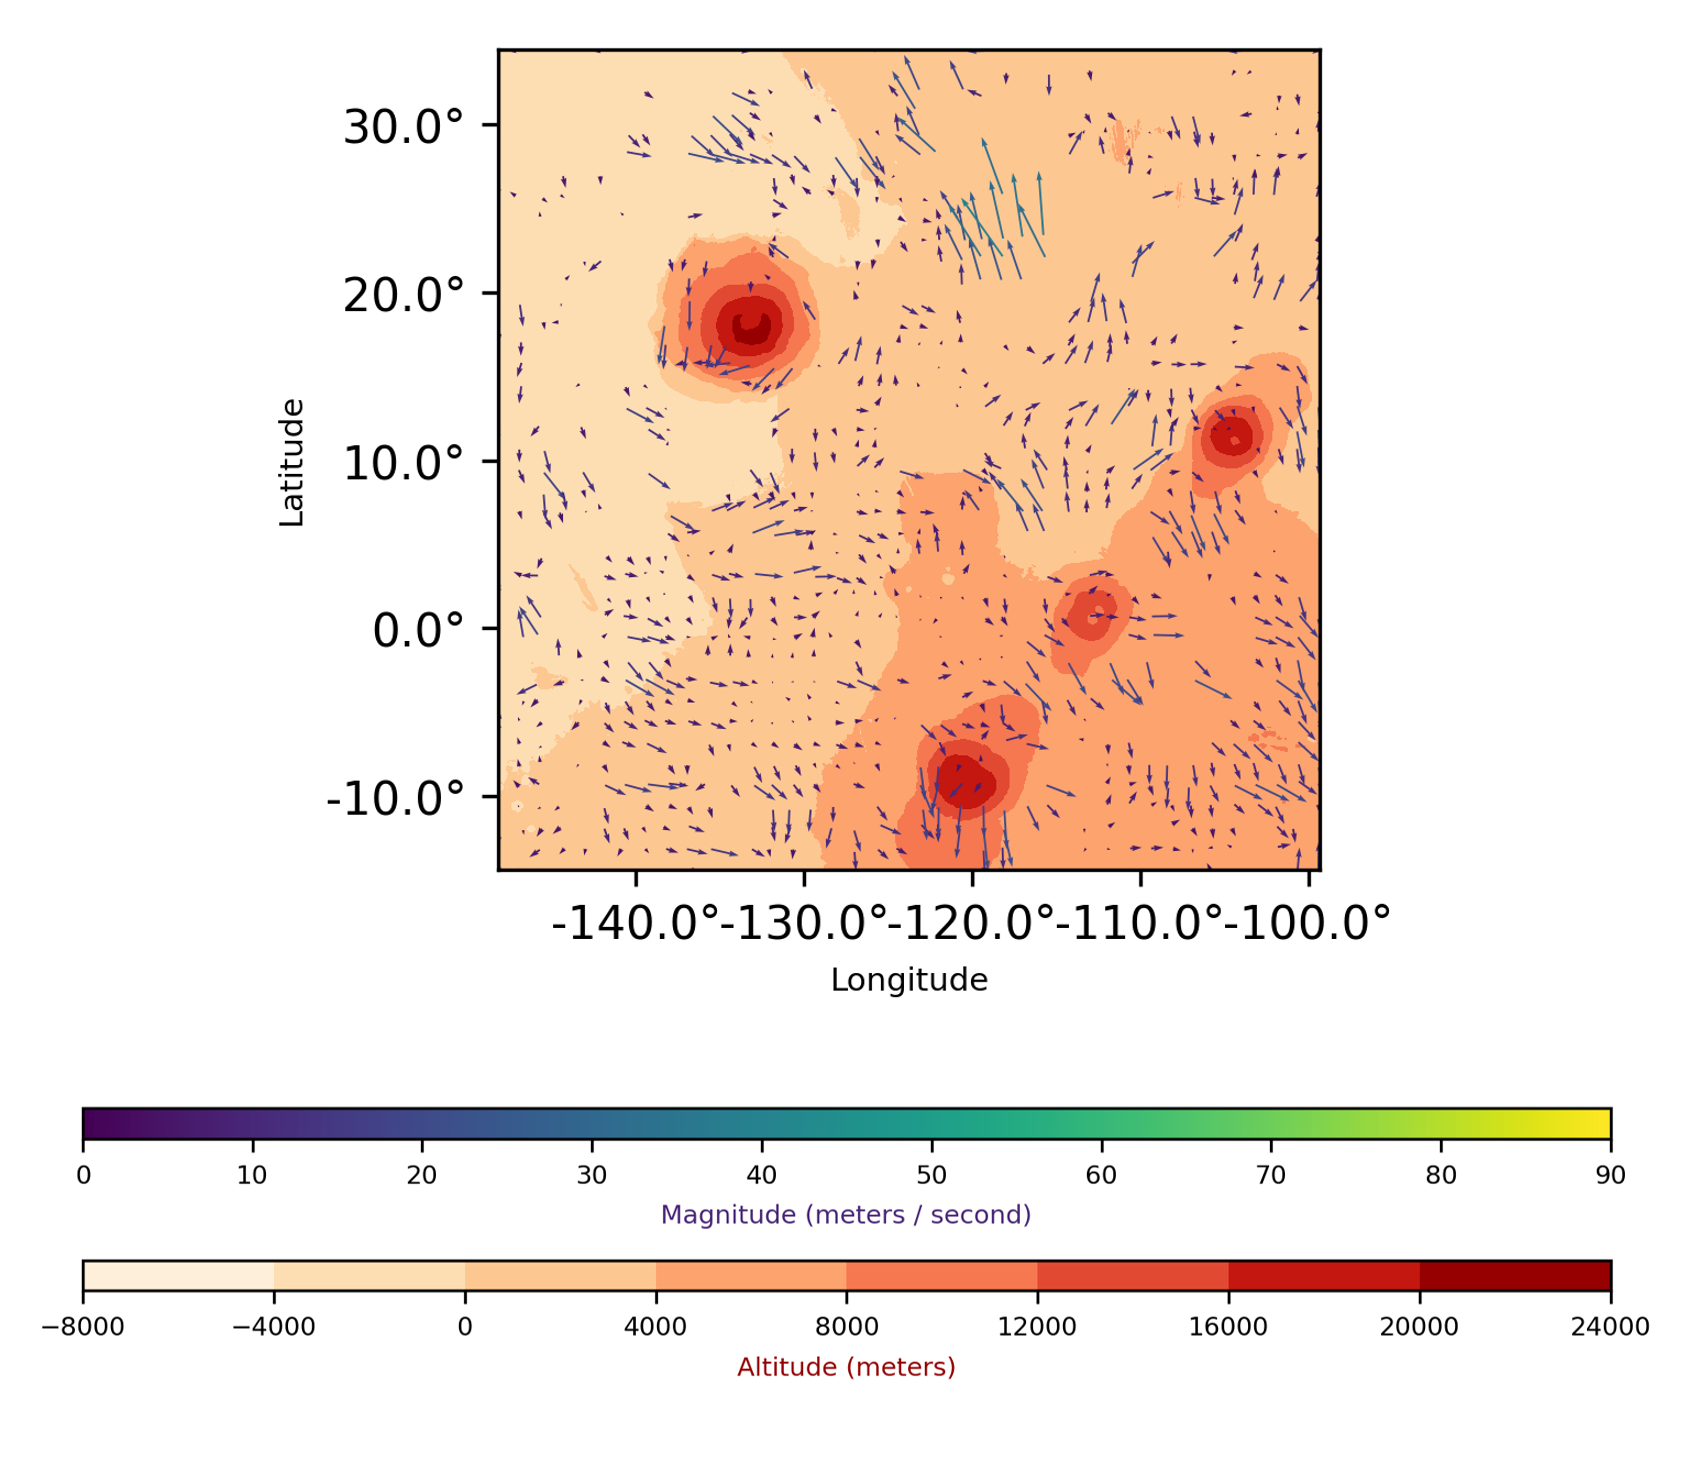
\includegraphics[width=1\textwidth]{fig_40.png}
    \caption{Velocity fields - UTC: 23/10/2023 10:56:50 - 11:26:53}
\end{figure}
\FloatBarrier
When comparing the wind fields in this thesis to those obtained by Shaimaa Ahmed AlBlooki in 2023 \cite{AlBlooki2023}, using a version of the data without pointing correction, some differences are noticeable. The wind field visualisations in this thesis display fewer vectors, potentially due to a higher correlation cut-off of 0.4 and different CIV parameters. Additionally, there are minor variations in vector locations, with some vectors present in Shaimaa Ahmed AlBlooki's results not appearing in this thesis’s wind fields, and the wind speeds in the 2023 thesis seem higher. Nevertheless, the overall wind directions remain consistent across both sets of wind field maps(see Figure 4.11).
\FloatBarrier
\begin{figure}[h!] 
    \centering
    \includegraphics[width=1\textwidth]{fig_41.png}
    \caption{Comparison of a wind field obtained in Shaimaa Ahmed AlBlooki 2023 thesis and this thesis - UTC: 22/11/2021 14:26:52 - 14:36:52}
\end{figure}
\FloatBarrier
Several trends are evident in the wind field visualizations (refer to Figure A.3 to A.8 for the complete sequences). In the northern hemisphere, winds tend to shift towards the northwest, particularly in the area left to approximately -140° longitude, near Olympus Mons. In contrast, winds in the southern hemisphere predominantly move southward. Additionally, in the southern hemisphere between longitudes of about -125° and -100°, there is a tendency for winds to shift towards the east.
Although wind speeds are generally higher in the Northern Hemisphere, there appears to be a pattern of symmetry in the wind field directions. This pattern suggests a possible mirrored symmetry relative to the equator, with a reversed orientation. The tendency for winds to shift northwards in the northern hemisphere and southwards in the southern hemisphere is also evident in the meridional plots shown in Figure A.2.
\chapter{Conclusion and Discussion\label{chap:conclusion}}

Understanding wind patterns on Mars is vital for advancing our knowledge of planetary atmospheric dynamics and planning future missions. In this thesis, four different image processing techniques and Correlation Image Velocimetry (CIV) were used to analyze the wind fields on Mars.

While the image processing methods applied in this thesis enhanced the visibility of clouds and led to some improvements in CIV results, they didn't provide a significant advantage over the original images.
However, the analysis revealed that CLAHE led to the detection of additional velocity vectors not apparent in other processing methods, indicating that enhancing sub-regions can be effective. 
Moreover, using pointing-corrected images versus non-pointing-corrected images does not affect the overall wind direction trends, which exhibit distinct patterns. However, the choice of CIV parameters and the image material used can significantly impact the results, as evidenced by noticeable differences between the CIV results in this thesis and those in Shaimaa Ahmed AlBlooki's thesis. In addition, several error factors need to be considered when analysing the wind fields, including uncertainty in the exact direction of the velocity vectors due to the 3-4 kilometer pixel resolution, variations in solar illumination, and potential spacecraft position instabilities.

To further enhance CIV results, future work could explore other pre-processing techniques, particularly those focusing on the enhancement of sub-regions within images. Additionally, high-pass filtered images suggested the presence of atmospheric waves, which warrants further investigation to potentially provide new insights into martian atmospheric dynamics.


\bibliography{references}
\appendix
\chapter{Appendix\label{chap:appendix}}

\begin{figure}[h!]
    \centering
    \includegraphics[width=0.9\textwidth]{appendix_a.png}
    \caption{First image of the image sequence from UTC: 24/12/2021 10:30:07. A high-pass filter was applied with different cut-off radii and the square root of pixel intensities was computed to enhance the result.}
\end{figure}
\FloatBarrier
\begin{figure}[h!]
    \centering
    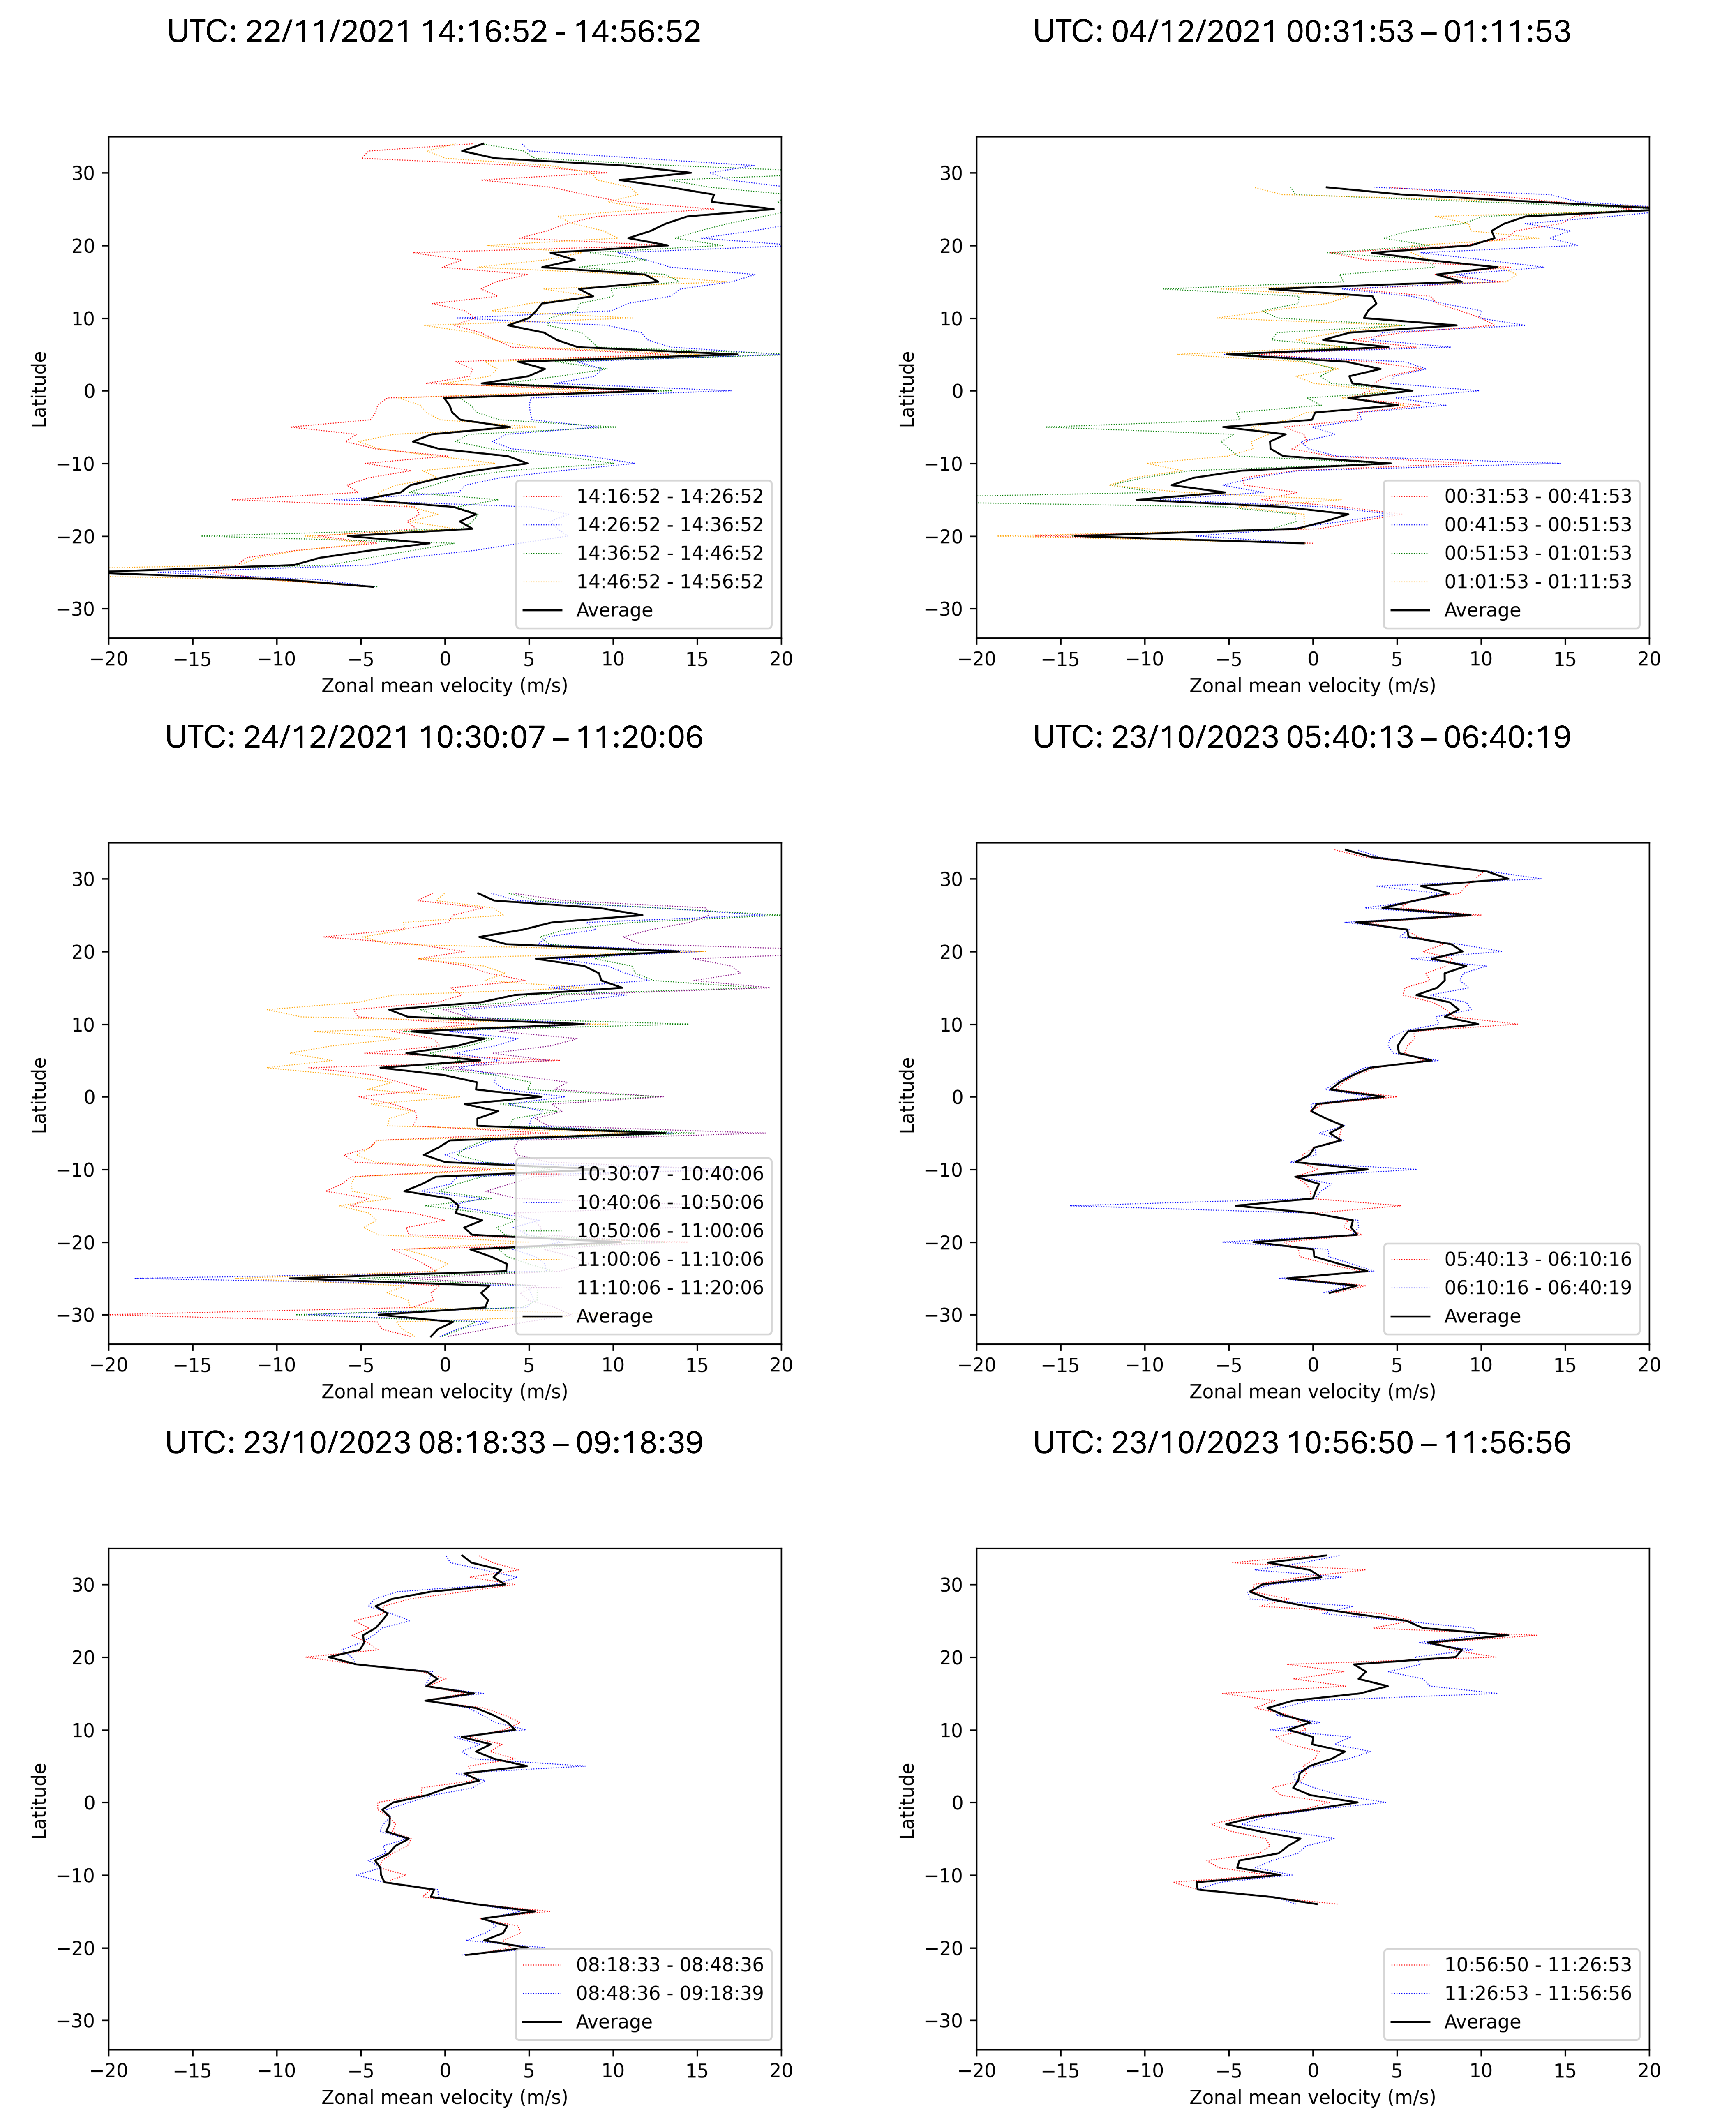
\includegraphics[width=0.9\textwidth]{appendix_b.png}
    \caption{Meridional plots of each image sequence displaying the north-south direction component of wind speeds as a function of latitude.}
\end{figure}
\FloatBarrier
\begin{figure}[h!]
    \centering
    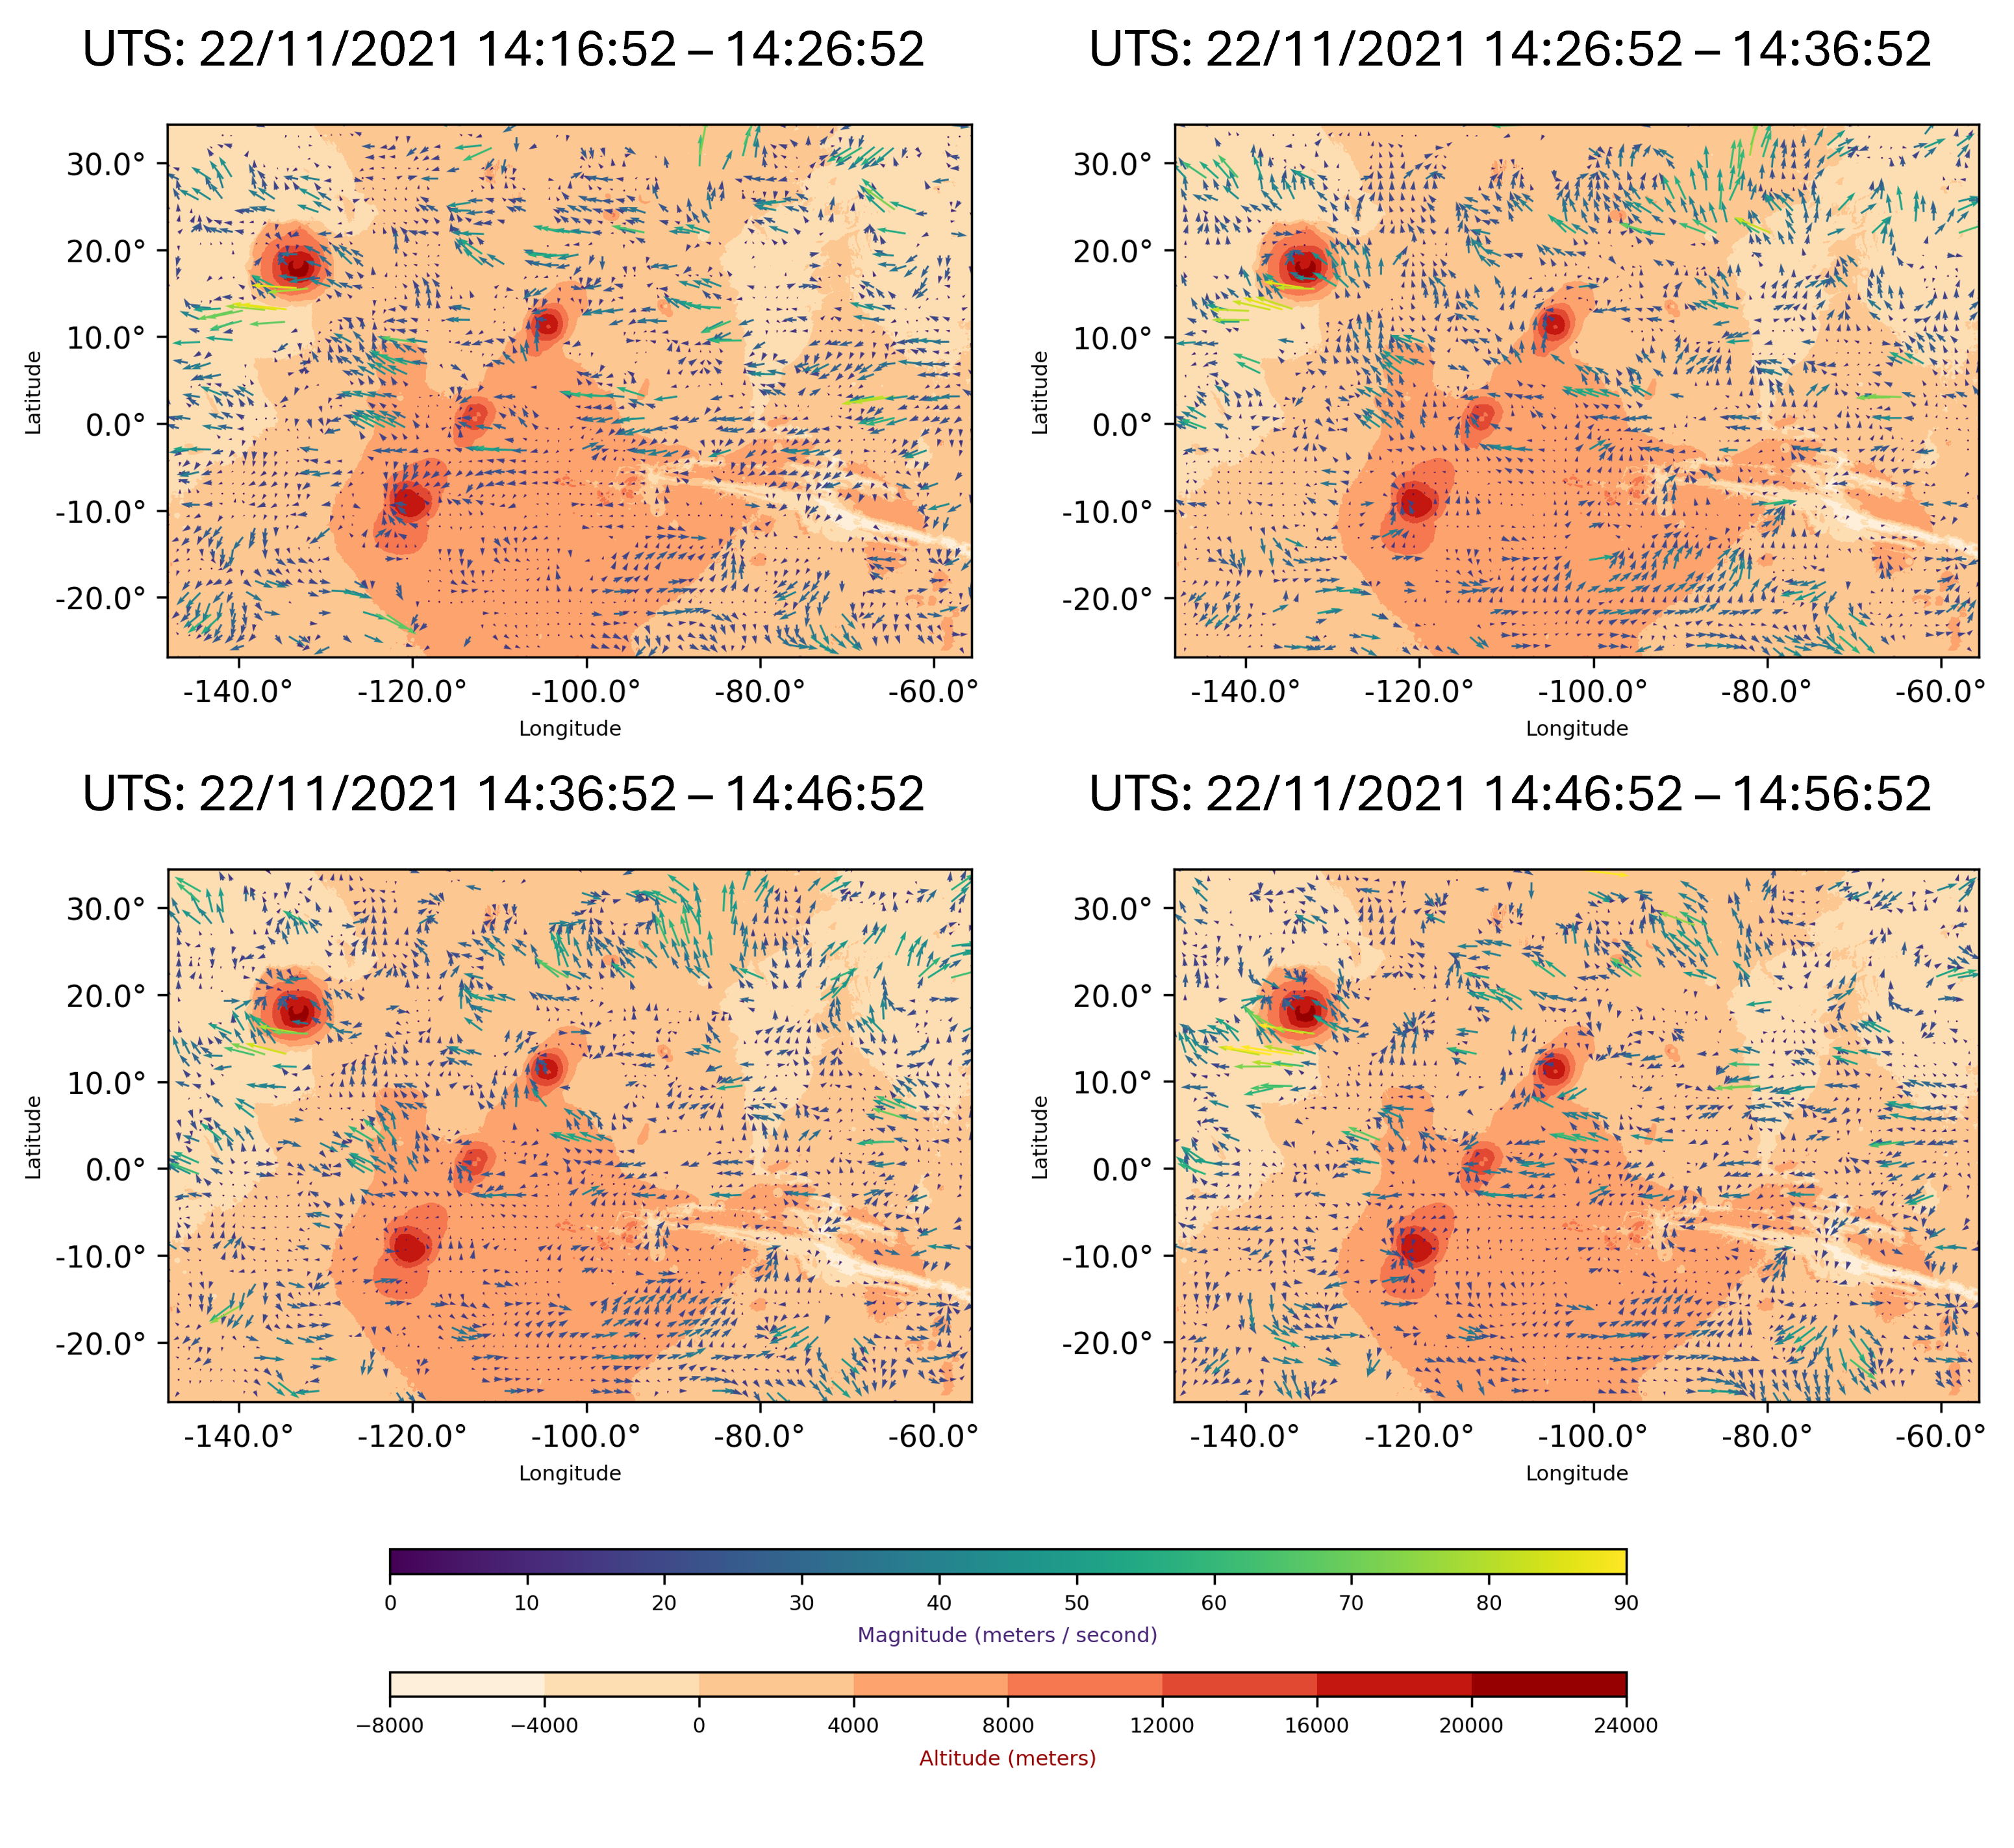
\includegraphics[width=0.9\textwidth]{appendix_c.png}
    \caption{Wind field results: UTC 22/11/2021 14:16:52 - 14:56:52}
\end{figure}
\FloatBarrier
\begin{figure}[h!]
    \centering
    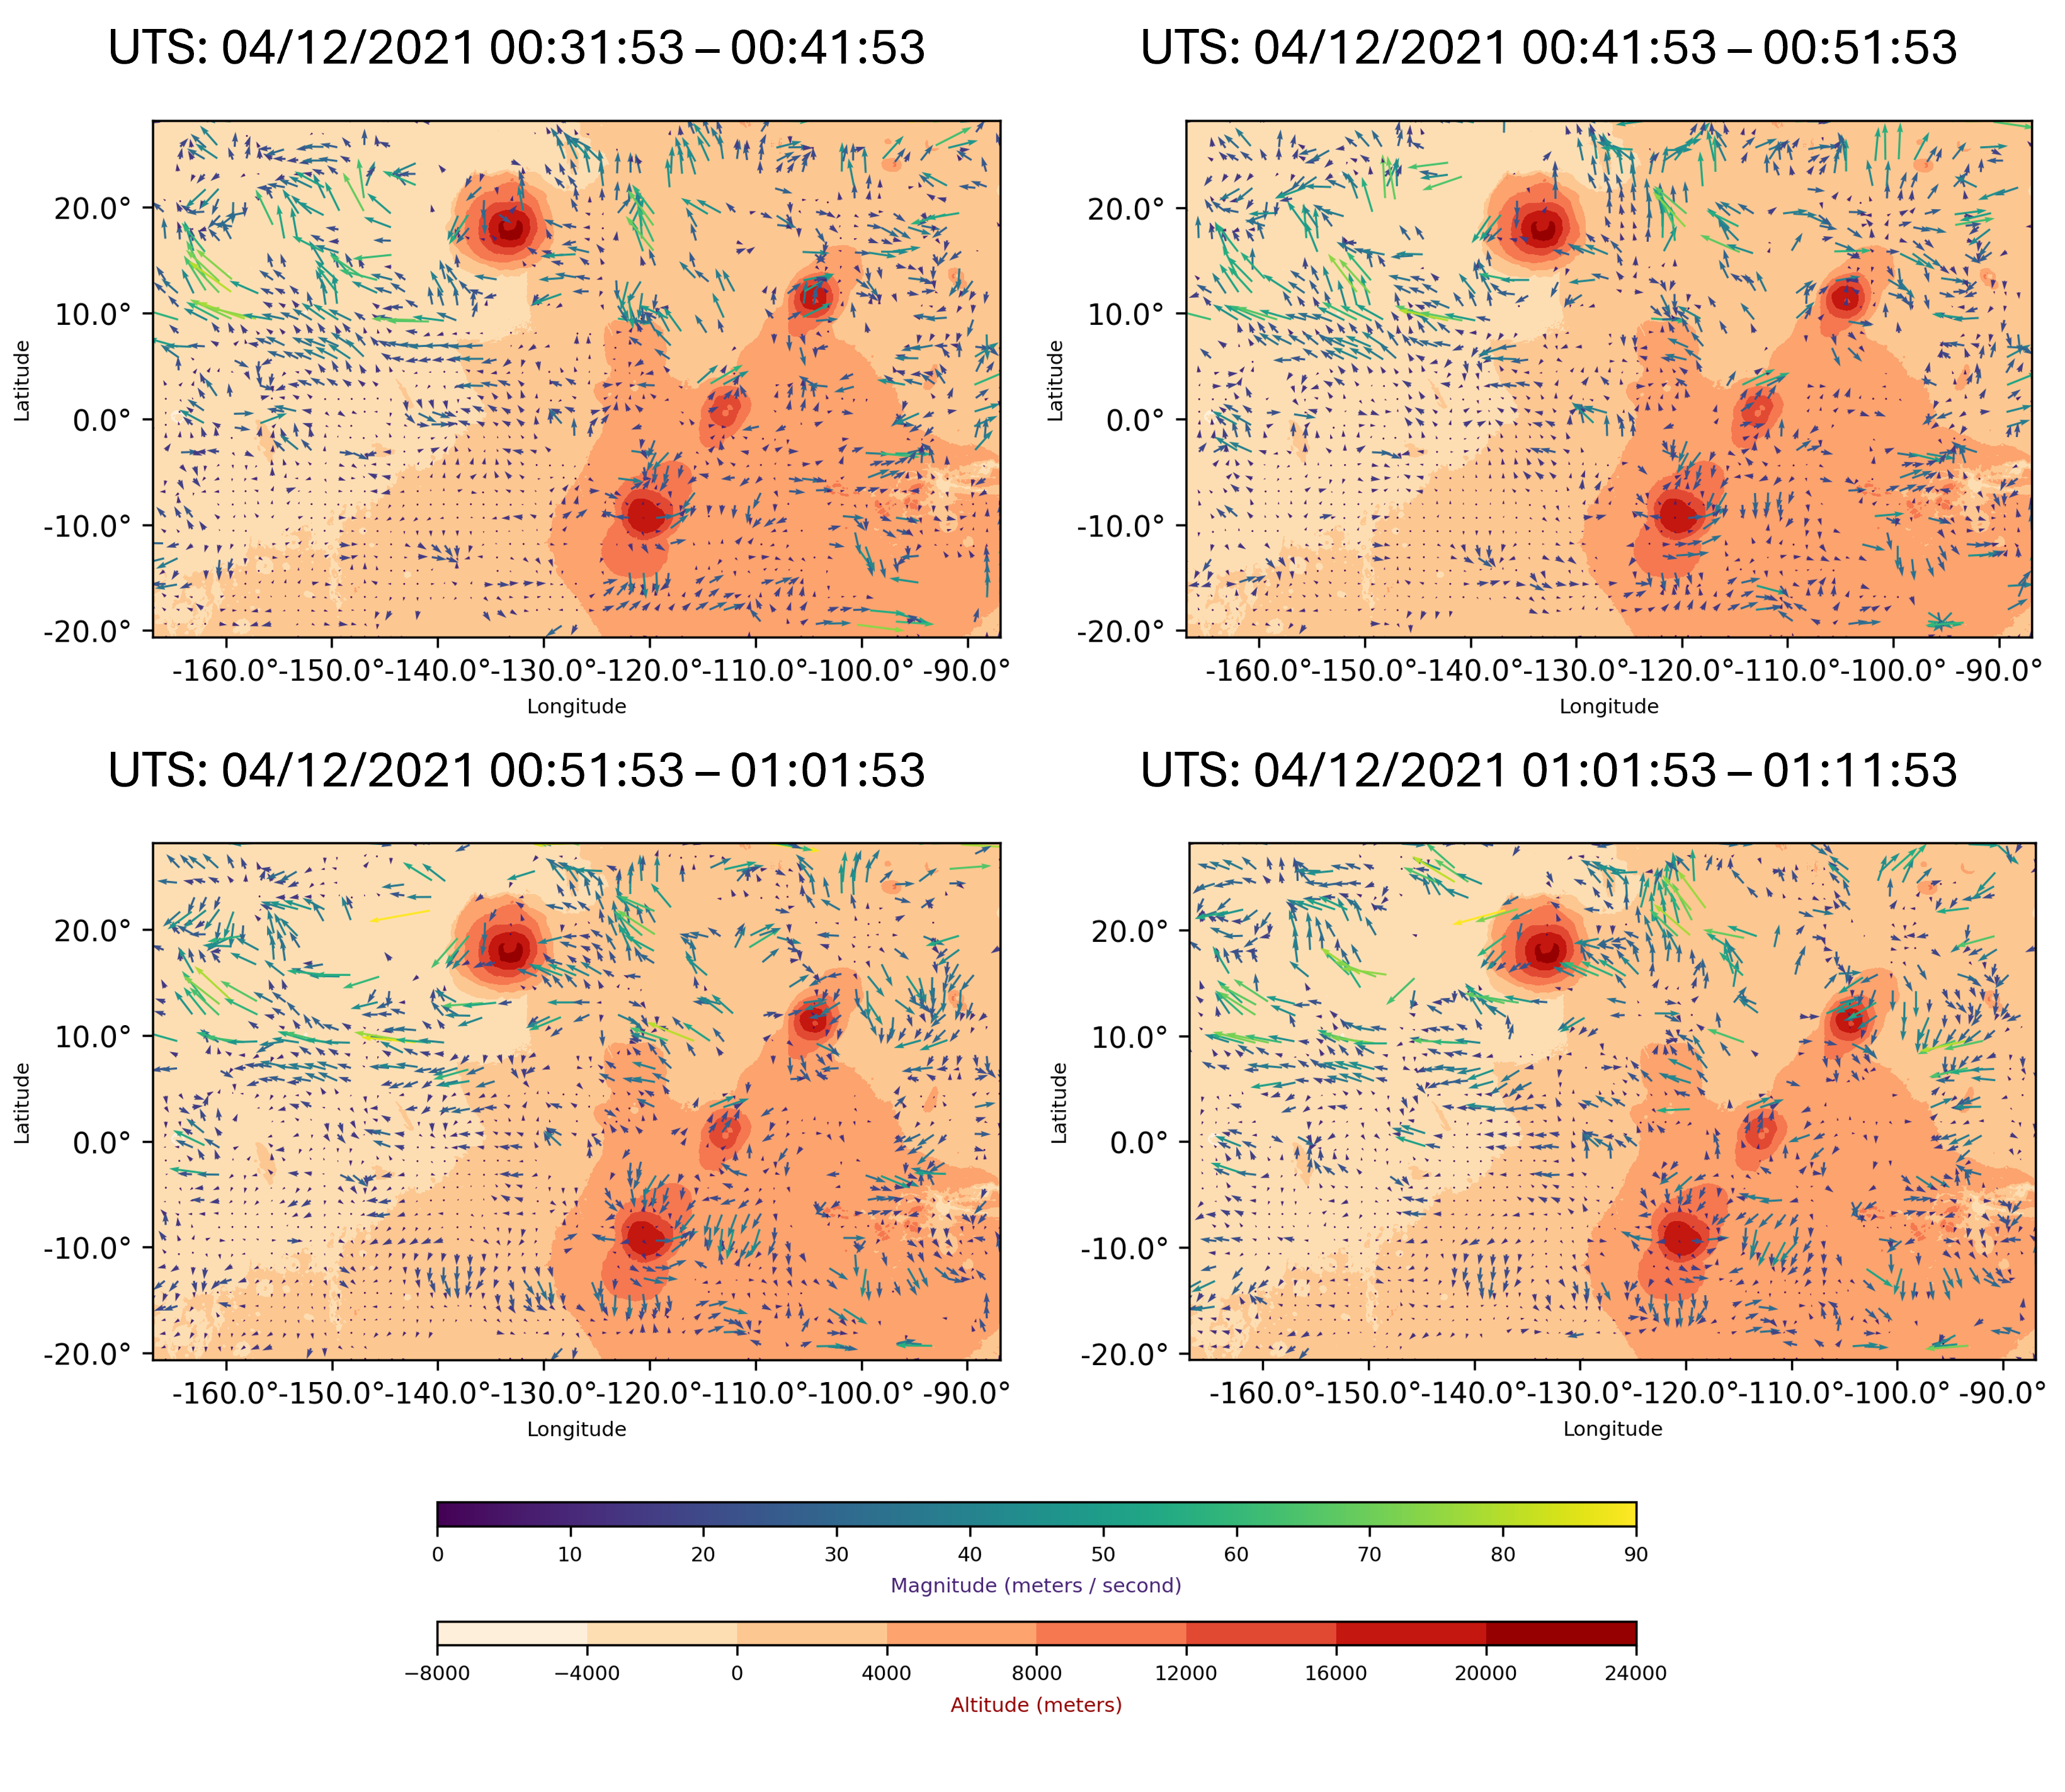
\includegraphics[width=0.9\textwidth]{appendix_d.png}
    \caption{Wind field results: UTC 04/12/2021 00:31:53 - 01:11:53}
\end{figure}
\FloatBarrier
\begin{figure}[h!]
    \centering
    \includegraphics[width=0.9\textwidth]{appendix_e.png}
    \caption{Wind field results: UTC 24/12/2021 10:30:07 - 11:20:06}
\end{figure}
\FloatBarrier
\begin{figure}[h!]
    \centering
    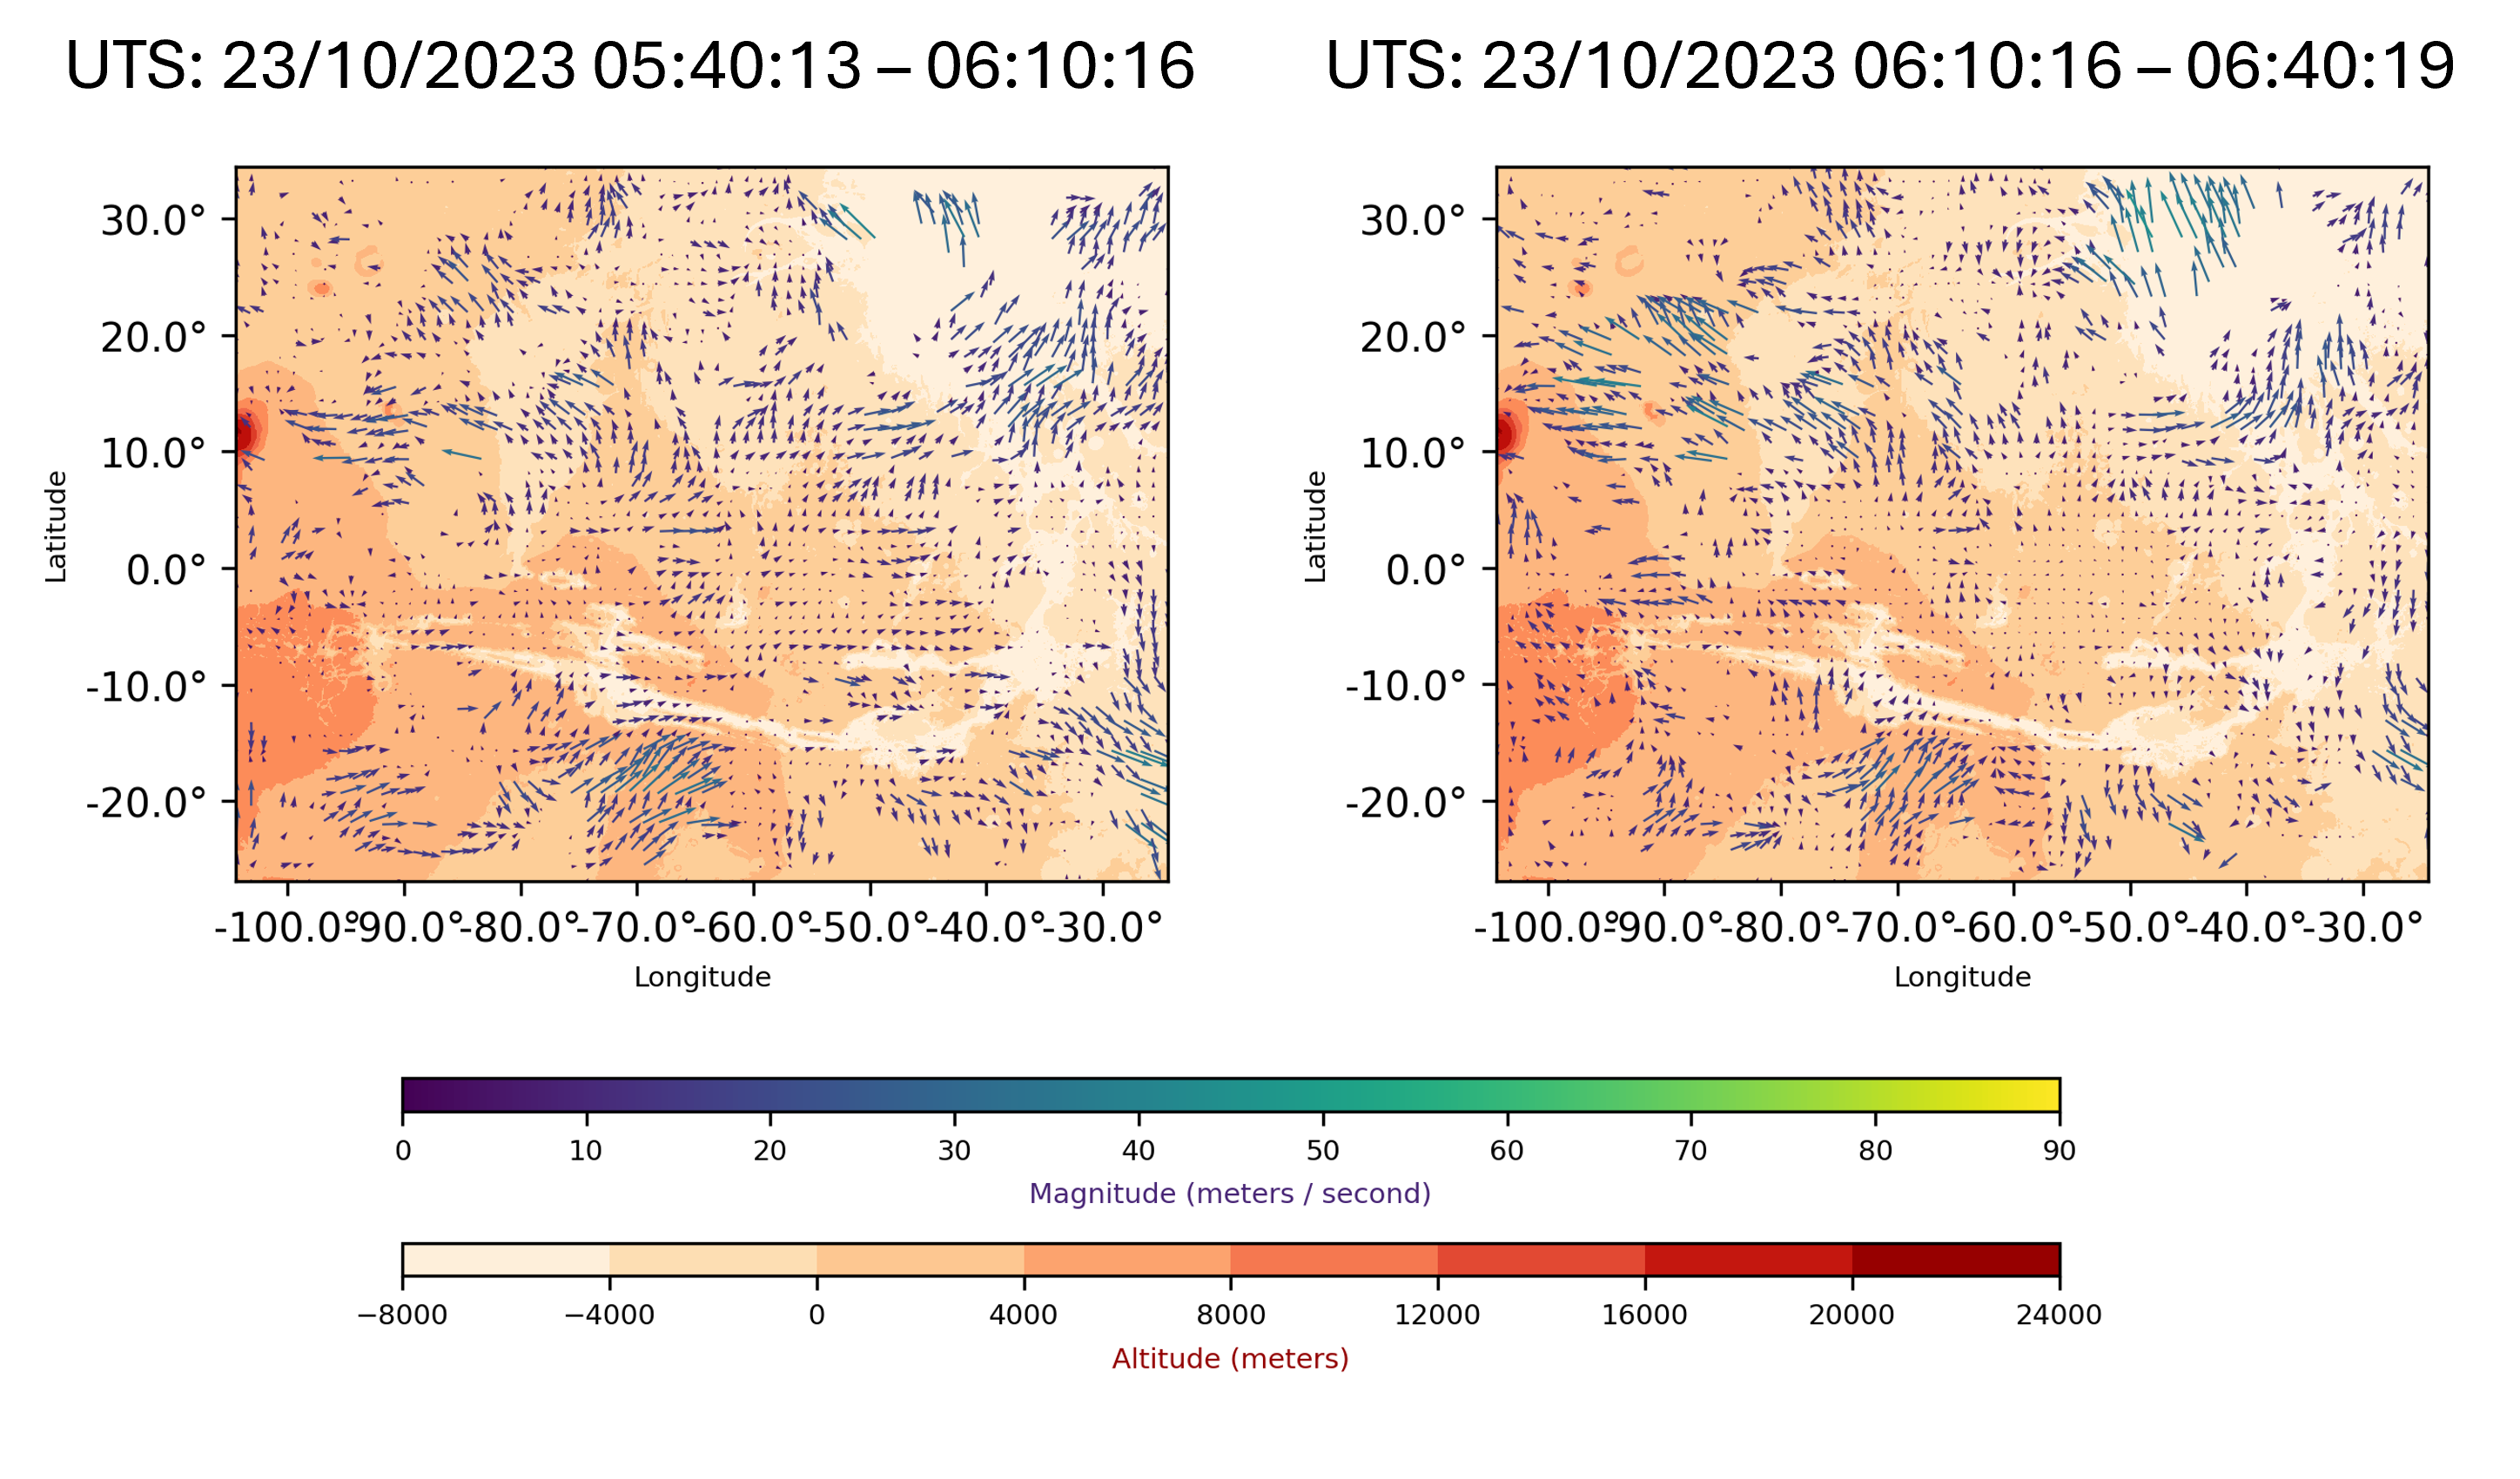
\includegraphics[width=0.9\textwidth]{appendix_f.png}
    \caption{Wind field results: UTC 23/10/2023 05:40:13 - 06:40:19}
\end{figure}
\FloatBarrier
\begin{figure}[h!]
    \centering
    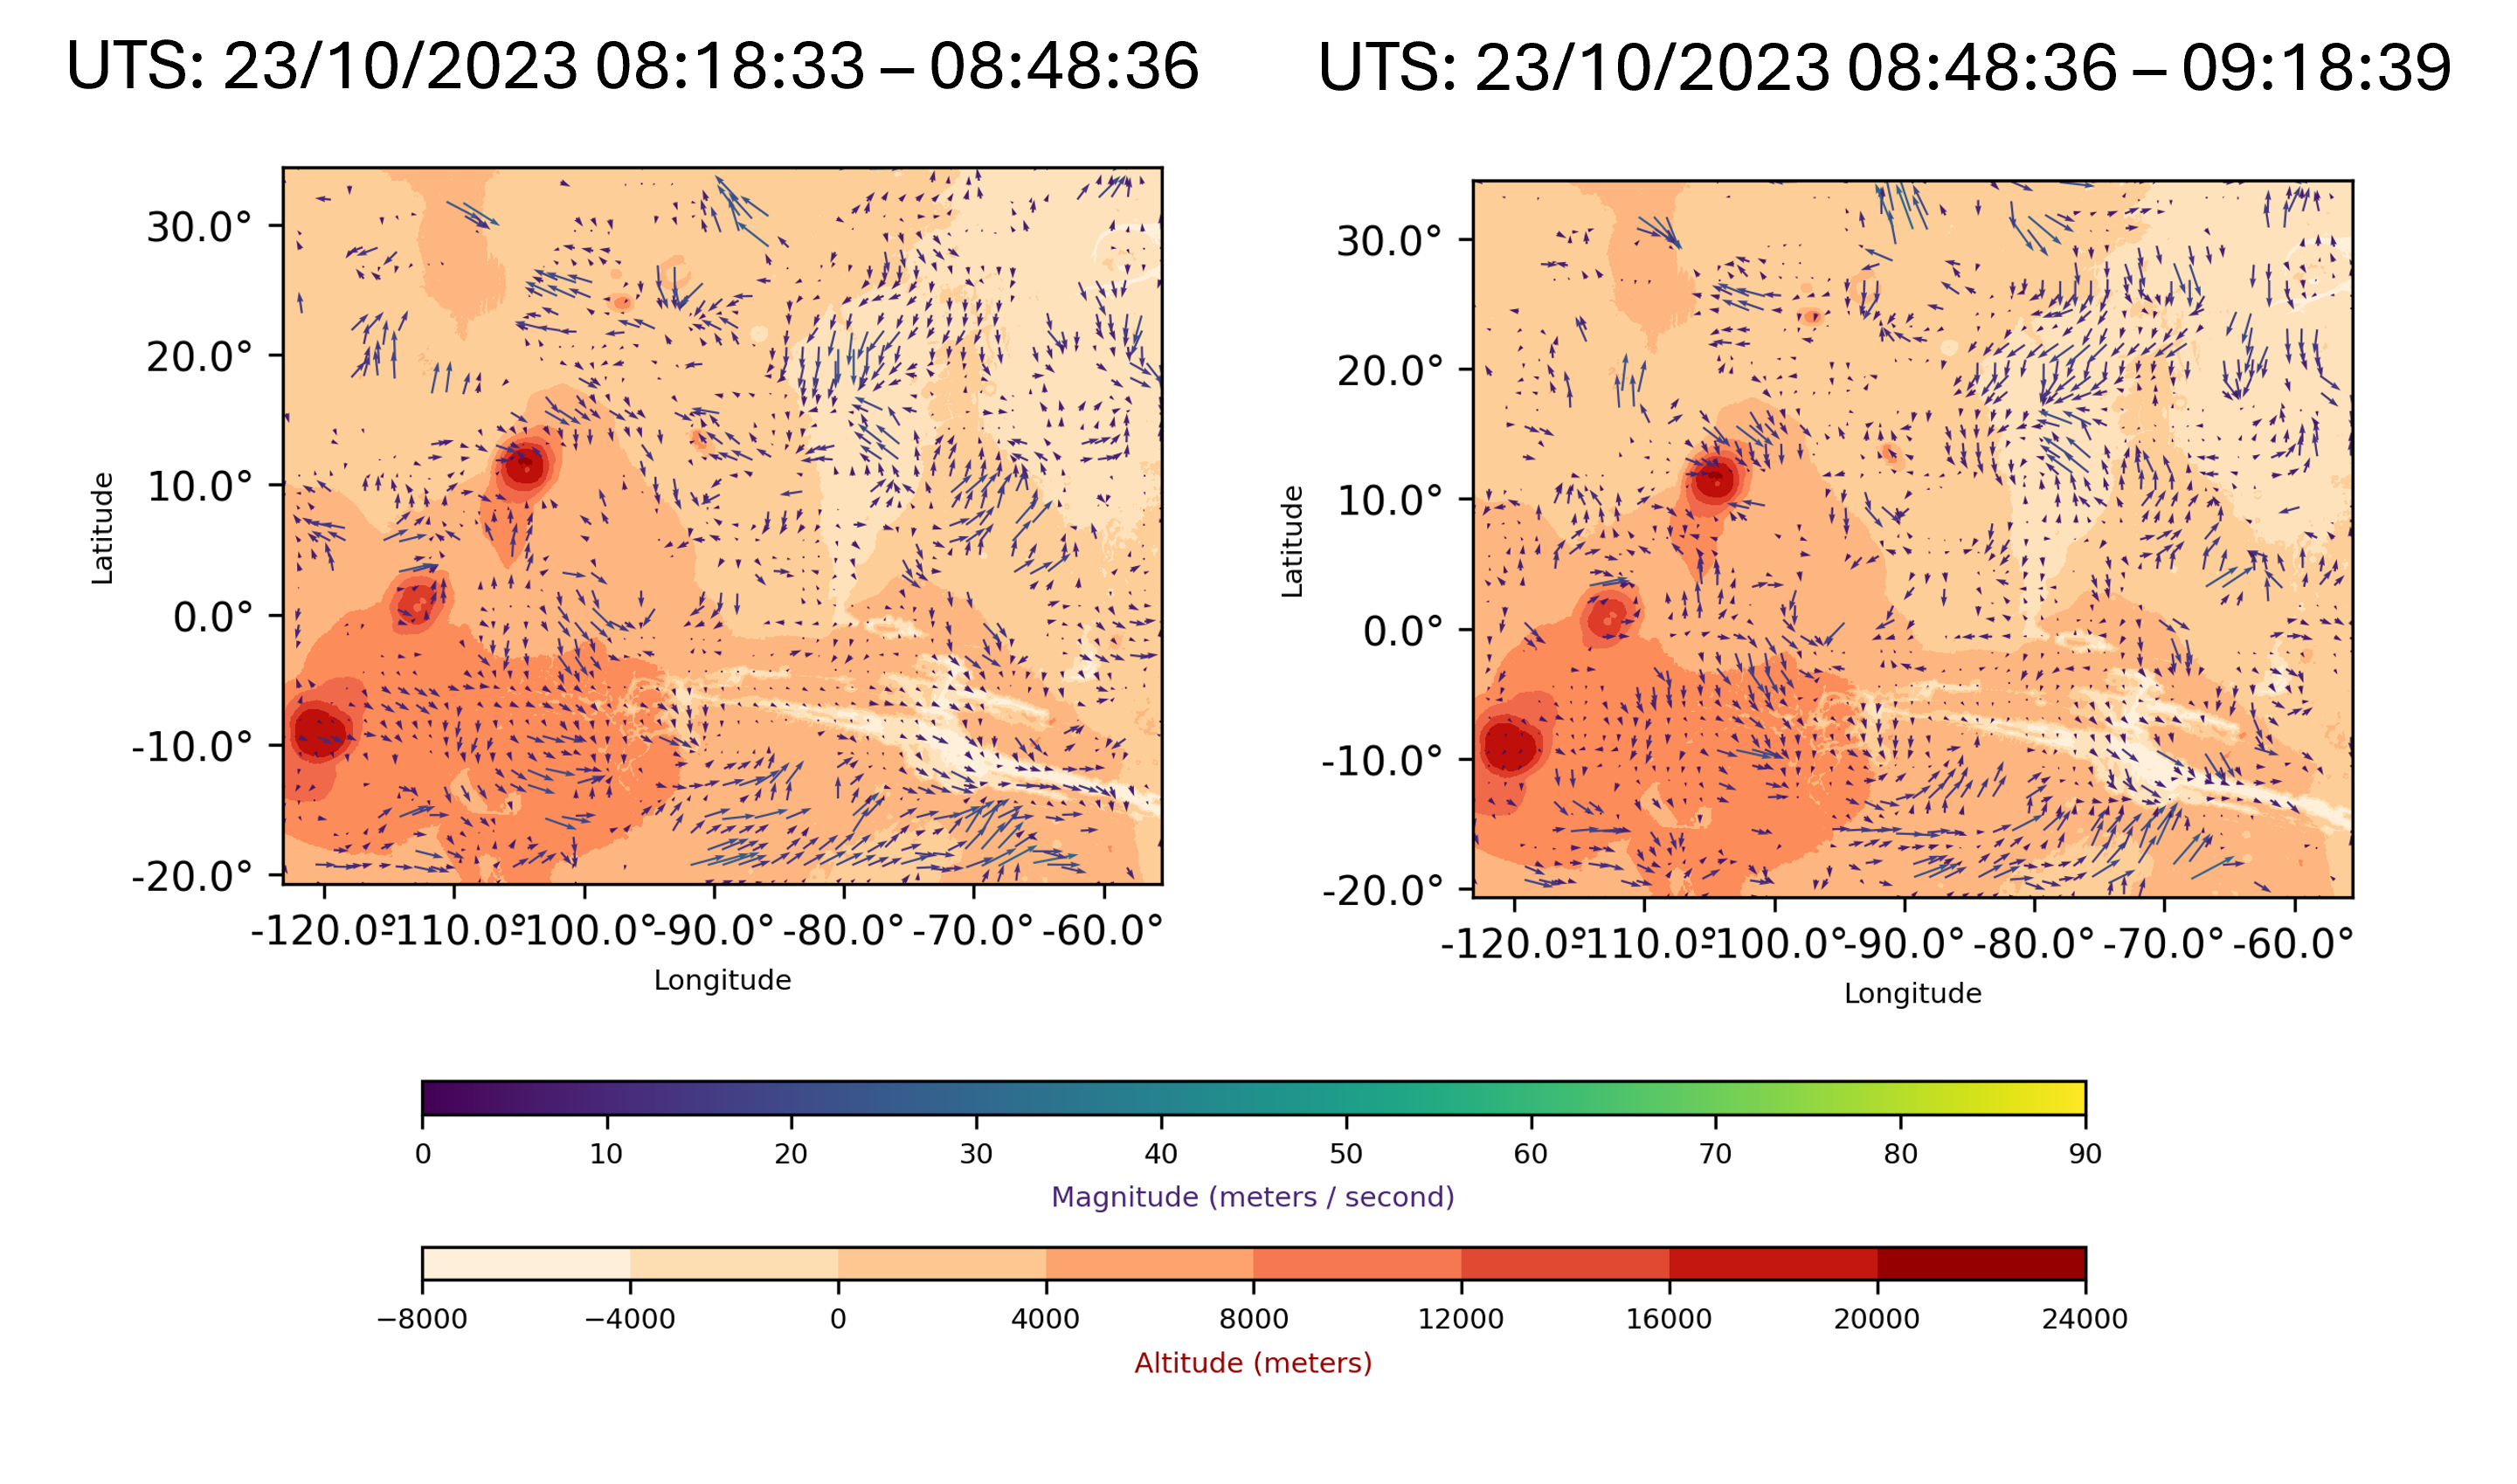
\includegraphics[width=0.9\textwidth]{appendix_g.png}
    \caption{Wind field results: UTC 23/10/2023 08:18:33 - 09:18:39}
\end{figure}
\FloatBarrier
\begin{figure}[h!]
    \centering
    \includegraphics[width=0.9\textwidth]{appendix_h.png}
    \caption{Wind field results: UTC 23/10/2023 10:56:50 - 11:56:56}
\end{figure}

\end{document}
